\documentclass[11pt]{article}


%\input{meta/packages}
%
\usepackage{cite}
\usepackage[T1]{fontenc}
\usepackage{times}
\usepackage{url}
\usepackage{amsmath}
\usepackage{fancyhdr}
\usepackage{fancyvrb}
\usepackage{fancybox}
\usepackage{color}
\usepackage{colortbl}
\usepackage[table]{xcolor}
%\usepackage{tex-helpers/mathpartir}
\usepackage{amssymb}
\usepackage{xspace}
\usepackage{comment}
\usepackage{graphicx}
\graphicspath{{figures/}}
\usepackage{epsfig}
\usepackage{wrapfig}
\usepackage{multirow}
\usepackage{subfig}

% Added listing for code listings
\usepackage{listings}
\usepackage{relsize}
\usepackage{setspace}
\usepackage{sidecap}
\usepackage{algorithm}
\usepackage{algorithmic}

\textwidth=16.5cm 
\textheight=22.5cm 
\textwidth=16.5cm 
\textheight=55.5pc
\topmargin=-0.5cm 
\headsep=0cm 
\headheight=0cm 
\oddsidemargin=0cm
\evensidemargin=0cm 
\marginparwidth=0cm
\parskip=0cm
\itemsep=0.1pt
\parindent=0.5cm

%Set table separation 
\setlength{\tabcolsep}{1pt}

% Allow figures to take up the entire page
\renewcommand\floatpagefraction{.99}
\renewcommand\topfraction{.99}
\renewcommand\bottomfraction{.90}
\renewcommand\textfraction{.01}   
\setcounter{totalnumber}{50}
\setcounter{topnumber}{50}
\setcounter{bottomnumber}{50}

% formatting for grammars
%\input{tex-helpers/obey}
%\input{tex-helpers/grammar}
%\renewcommand{\nonterm}[1]{\mbox{\textit{#1}}}
\newcommand{\oneormore}[1]{#1\ensuremath{^+}}

\newcommand{\opt}[1]{\textbf{[}#1\textbf{]}}

\newcommand{\mc}[1]{\mbox{\rm \ensuremath{\text{\code{#1}}}}} 
\newcommand{\loc}{\ensuremath{\mathord{\mathit{loc}}}}
\newcommand{\ec}{\ensuremath{\mathop{\mathbb{E}}}}
\newcommand{\hole}{\ensuremath{\mathord{\mathit{-}}}}
\newcommand{\reducesto}{\hookrightarrow}

\newcommand*{\seq}[1]{\ensuremath{\left\langle {#1} \right\rangle}}
\newcommand{\config}{\seq}
\newcommand{\udot}{\mathbin{\sqcup \kern-0.53em \cdot \,}}

% Aux functions
\newcommand{\auxFunc}[1]{\ensuremath{\mathop{\mathit{#1}}}}
\newcommand{\concat}{\auxFunc{concat}}
\newcommand{\reverse}{\auxFunc{reverse}}

% Type checking macros
% change symbol type of : from mathrel 
%\DeclareMathSymbol{:}{\mathbin}{operators}{"3A} 
\newcommand{\OK}{\mbox{OK}}
\newcommand{\OKin}{\mbox{OK in }}
\newcommand{\isType}{\mbox{\textit{isType}}}
\newcommand{\isThunkType}{\mbox{\textit{isThunkType}}}
\newcommand{\isClass}{\mbox{\textit{isClass}}}
\newcommand{\Types}{\mbox{\textit{Types}}}
\newcommand{\Names}{\mbox{\textit{Names}}}
\newcommand{\TypeEnv}{\mbox{\textit{TypeEnv}}}
\newcommand{\VD}{\mbox{\textit{VD}}}
\newcommand{\TypesInOrder}{\mbox{\textit{typesInOrder}}}
\newcommand{\dom}{\mbox{\textit{dom}}}
\newcommand{\rng}{\mbox{\textit{rng}}}
\newcommand{\POWERSET}[1]{\mbox{\textit{PowerSet}}(#1)}
\newcommand{\delete}{\mbox{\textit{delete}}}
\newcommand{\mklist}{\mbox{\textit{mksupers}}}
\newcommand{\uminus}{\mbox{$\cup\!\!\!\!-$}}
\newcommand{\iminus}{\mbox{$\cap\!\!\!\!-$}}
\newcommand{\rname}[1]{$\TirName{(#1)}$} % for inline inferrule names
\newcommand{\STO}{\ensuremath{<:}}  % ``subtype of''
\newcommand{\consistent}{\ensuremath{\approx}}

% Notations 
\newcommand{\produces}{\rightsquigarrow}
\newcommand{\refinedBy}{\sqsubseteq}

% Macros for the Figure Editor Example
\newcommand{\FElement}{\mbox{\texttt{FElement}~}}
\newcommand{\ChangedFE}{\mbox{\texttt{changedFE}~}}
\newcommand{\FEChange}{\mbox{\texttt{FEChange}~}}


% Macros for defining phase transition analysis
\newcommand{\cfg}{\ensuremath{{\cal CFG}}\xspace}
\newcommand{\globTypeMap}{\ensuremath{T}\xspace}

%Redefinition of some math commands widely used outside
%mathmode
\newcommand{\memOf}{\ensuremath{\in}\xspace}

% Help LaTeX not violate the column margins
\tolerance=50000

% settings for listings
\definecolor{lightgray}{gray}{0.97}
\definecolor{darkgray}{gray}{0.5}
\definecolor{OliveGreen}{cmyk}{0.64,0,0.95,0.40}
\definecolor{DarkGreen}{cmyk}{0.58,0,0.66,0.26}
\definecolor{LightRed}{cmyk}{0,0.682,0.728,0}
\definecolor{purple}{cmyk}{0.41,0.73,0,0}

\lstset{
	language=bash, emph={},
	mathescape=false, escapechar=@,
	backgroundcolor=\color{lightgray},
	commentstyle=\color{darkgray},
	keywordstyle=\color{OliveGreen}\bfseries,
	basicstyle=\relsize{-3}\sffamily,
	numberstyle=\scriptsize\sffamily,
	emphstyle=\color{purple},
	emphstyle={[2]\color{LightRed}},
	commentstyle=\color{DarkGreen},
	stringstyle=\color{OliveGreen},
	numbers=left, stepnumber=1,
	numberblanklines=false,
	numberstyle=\tiny,
	numbersep=-3pt,
	frame=none, framexleftmargin=0pt, framexrightmargin=0pt, 
	%xleftmargin=15pt, xrightmargin=4pt,
	columns=flexible, breaklines=true,
	showspaces=false, showstringspaces=false, showtabs=false, tabsize=2,
	morekeywords={input,exists,foreach,ifall,output,of,weight,stop,visit,before,after},
	emph={int,string,bool,time,array,stack,map,visitor,%
true,false,%
top,sum,mean,maximum,minimum,set,collection,%
Project,CodeRepository,Revision,ChangedFile,ASTRoot,Namespace,Declaration,Type,Method,Variable,Statement,Expression,Modifier,%
ExpressionKind,NEW,LITERAL,EQ,NEQ,%
TypeKind,CLASS,ANONYMOUS,%
ModifierKind,OTHER,%
ChangeKind,DELETED,%
StatementKind,IF,%
RepositoryKind,SVN},
	emph={[2]isfixingrevision,getast,iskind,hasfiletype,isliteral,getsnapshot,has_modifier_public,%
format,def,len,match,lowercase,yearof,haskey,remove,strfind,push,pop},
}

% could use \relsize{-2} instead of \scriptsize below
\newcommand{\FIGCODEFONT}{\relsize{-2.5}\ttfamily}

% cross referencing
%\newcommand{\algref}[1]{Algorithm~\ref{#1}}
%\newcommand{\figref}[1]{Figure~\ref{#1}\xspace}
%\newcommand{\tabref}[1]{Table~\ref{#1}\xspace}
%\newcommand{\fignref}[1]{Figure~\ref{#1}\xspace}
%\newcommand{\secref}[1]{Section~\ref{#1}\xspace}
%\newcommand{\secnref}[1]{Section~\ref{#1}\xspace}

%\newcommand{\etal}{~\textit{et al.}\@\xspace}
\newcommand{\kind}{\textit{kind}\xspace}
\newcommand{\KIND}{\textit{KIND}\xspace}

\newcommand{\lang}{\textit{Boa}\@\xspace}

% Theorems environments...
%{theorems}
\newtheorem{theorem}{Theorem}[section]
\newtheorem{axiom}[theorem]{Axiom}
\newtheorem{corollary}[theorem]{Corollary}
\newtheorem{definition}[theorem]{Definition}
\newtheorem{example}[theorem]{Example}
\newtheorem{fact}[theorem]{Fact}
\newtheorem{lemma}[theorem]{Lemma}
\newtheorem{proposition}[theorem]{Proposition}
\newtheorem{remark}[theorem]{Remark}
\newtheorem{conjecture}[theorem]{Conjecture}
% Some helpful notation
\newcommand{\PROOF}{{\em Proof:\/}~~}
\newcommand{\PROOFSKETCH}{{\em Proof Sketch:\/}~~}
\newcommand{\QED}{\rule{0.4em}{0.65em}}

\definecolor{light-gray}{gray}{0.9}
\definecolor{very-light-gray}{gray}{0.95}

% Change section headings to look nicer
\makeatletter
\renewcommand\thesection{{\large\Alph{section}.}}
\renewcommand\section{\@startsection {section}{1}{\z@}%
                                   {-3.5ex \@plus -1ex \@minus -.2ex}%
                                   {2.3ex \@plus.2ex}%
                                   {\large\scshape\bf}}
\makeatother

\renewcommand\thesubsection{{\normalsize\Alph{section}.}{\normalsize\arabic{subsection}}}

\makeatletter
\renewcommand\subsection{\@startsection {subsection}{1}{\z@}%
                                   {-3.5ex \@plus -1ex \@minus -.2ex}%
                                   {2.3ex \@plus.2ex}%
                                   {\normalsize\scshape\bf}}
\makeatother

\renewcommand\thesubsubsection{{\normalsize\Alph{section}.}{\normalsize\arabic{subsection}.}{\normalsize\arabic{subsubsection}}}

\makeatletter
\renewcommand\subsubsection{\@startsection {subsubsection}{1}{\z@}%
                                   {-3.5ex \@plus -1ex \@minus -.2ex}%
                                   {2.3ex \@plus.2ex}%
                                   {\normalsize\scshape\bf}}
\makeatother

\newcommand\para[1]{\vspace{-1em}\paragraph{#1\ }}

% Different font in captions
\newcommand{\captionfonts}{\footnotesize}

% formatting of initial section quotations
\newcommand{\QUOTATION}[1]{\begin{flushright}\begin{footnotesize}\emph{#1}\end{footnotesize}\end{flushright}}
 
\makeatletter  % Allow the use of @ in command names
\long\def\@makecaption#1#2{%
  \vskip\abovecaptionskip
  \sbox\@tempboxa{{\captionfonts #1: #2}}%
  \ifdim \wd\@tempboxa >\hsize
    {\captionfonts #1: #2\par}
  \else
    \hbox to\hsize{\hfil\box\@tempboxa\hfil}%
  \fi
  \vskip\belowcaptionskip}
\makeatother   % Cancel the effect of \makeatletter

%\usepackage[ps2pdf,bookmarks=true]{hyperref}

\definecolor{light-gray}{gray}{0.9}
\definecolor{dark-gray}{gray}{0.7}

\newcommand\doctitle[1]{\newpage \setcounter{page}{1}\thispagestyle{fancyplain} \headheight=14pt%
                        \fancyhead[C]{\large{\bf #1}}\xspace\vspace{0.5em}}


                                                                        


\usepackage{graphicx,times}
\usepackage{wrapfig}
\usepackage{amsmath,epsfig}
\usepackage{setspace,array}
\usepackage{cite}
\usepackage{listings}
\usepackage{booktabs}
%\usepackage{bibentry}
\lstset{basicstyle=\scriptsize\sffamily,language={},frame=single,breaklines=true,columns=fullflexible,mathescape=true,escapechar=@}

\usepackage{tikz}
\newcommand*\circled[1]{\tikz[baseline=(char.base)]{
		\node[shape=circle,draw,inner sep=0.45pt] (char) {#1};}}


\usepackage{xspace}
%\usepackage{enumitem}

\usepackage{sectsty}
\sectionfont{\large}
\subsectionfont{\normalsize}
\subsubsectionfont{\normalsize}

\usepackage[compact]{titlesec}
\usepackage[skins]{tcolorbox}

\renewcommand{\theequation}{\thesection.\arabic{equation}}
\renewcommand{\baselinestretch}{1.0}

\newcommand*\rotdia{\multicolumn{1}{R{45}{1em}}}% no optional argument here, please!
\newcommand*\rot{\rotatebox{90}}
\usepackage{multicol,multirow}

\newtheorem{Definition}{Definition}
\newtheorem{Claim}{Claim}
\newtheorem{Lemma}{Lemma}
\newtheorem{Theorem}{Theorem}
\newtheorem{Property}{Property}
\newtheorem{Problem}{Problem}


\newcommand\aName[1]{{\small\textsc{#1}}\xspace}

% cross referencing
\newcommand{\figref}[1]{Figure~\ref{#1}}
\newcommand{\secref}[1]{Section~\ref{#1}}
\newcommand{\tabref}[1]{Table~\ref{#1}}
\newcommand{\defref}[1]{Definition~\ref{#1}}

%\newcommand\aName[1]{{\small\textnormal{\textsc{#1}}}\xspace}

%\newcommand\MUBench[0]{\aName{MuBench}}
\newcommand\MUDetect[0]{\aName{MuDetect}}



\newcommand\MUBench[0]{\aName{MuBench}}
\newcommand\MUPipe[0]{\aName{MuPipe}}
\newcommand\MUC[0]{\aName{MuC}}
\newcommand\AUG[0]{\aName{AUG}}

\newcommand{\etal}{{\em et al.}}

\newcommand\GROUM[0]{\aName{GROUM}}
\newcommand\eGROUM[0]{\aName{AUG}}
\newcommand\miner[0]{\aName{AUGMiner}}

\newcommand\Colibri[0]{\aName{Colibri/ML}}
\newcommand\DroidAssist[0]{\aName{DroidAssist}}
\newcommand\GraPacc[0]{\aName{GraPacc}}
\newcommand\GROUMiner[0]{\aName{GROUMiner}}
\newcommand\Jadet[0]{\aName{Jadet}}
\newcommand\PRMiner[0]{\aName{PR-Miner}}
\newcommand\CARMiner[0]{\aName{CAR-Miner}}
\newcommand\Alattin[0]{\aName{Alattin}}
\newcommand\Tikanga[0]{\aName{Tikanga}}
\newcommand\DMMC[0]{\aName{DMMC}}
\newcommand\RGJ[0]{\aName{RGJ07}}
\newcommand\Chronicler[0]{\aName{Chronicler}}
\newcommand\Acharya[0]{\aName{AX09}}

\newcommand{\checkNum}[1]{#1}

\newcommand{\revise} {\bf}

\newcommand{\code}[1]{{\scriptsize\texttt{#1}}}
\newcommand{\op}{\tau}
\newcommand{\refac}{\rho}
\newcommand{\edit}{\sigma}
\newcommand{\T}{\theta}
\newcommand{\comp}{;}
\newcommand{\pre}{\prec_P}
\newcommand{\meth}{KSISA}

\newcommand{\MyParagraph}[1]{\textbf{#1}{ }}
\newcommand{\fixme} [1] {\textcolor{red}{{\it FIXME}: #1}}

\usepackage{vmargin}
\setpapersize{USletter}
\setmarginsrb{1.0in}{1in}{1.0in}{1in}%
           {0pt}{0mm}{0pt}{10mm}
\newcommand{\remove}[1]{}



\usepackage{tweaklist}
\renewcommand{\enumhook}{\setlength{\topsep}{0pt}%
  \setlength{\itemsep}{0pt}}
\renewcommand{\itemhook}{\setlength{\topsep}{0pt}%
  \setlength{\itemsep}{0pt}}
\renewcommand{\descripthook}{\setlength{\topsep}{0pt}%
  \setlength{\itemsep}{0pt}}



%\newcommand\Tone{Thrust 1 (T1). Ongoing Evaluation of Existing Code Representation Learning in Bug Detect-Fix Processes}
\newcommand\Tone{Thrust 1 (T1). Design Framework and Environment for Code Representation Learning (CRL): Representations, Models, and Methodologies}

\newcommand\Ttwo{Thrust 2 (T2). Quality Evaluation Framework for Code Representation Learning}

\newcommand\Tthree{Thrust 3 (T3). Applications of CRL Framework in Bug Detection, Testing, Fault Localization, and Auto Program Repair}

%Enhancing Techniques in the Bug Fixing Process with Deep Learning}

% all tool names used in this proposal

%\newcommand\tool{NeuralPPA}

\newcommand{\tool}{\textsc{LLM--V2C}\xspace}

\begin{document}

\begin{center}
%{\large \bf Collaborative Research: SHF: Small: Innovations in Deep Learning to Enhance Program Analysis and Representations to Improve Bug Fixing Process}

%{\large \bf Collaborative Research: SHF: Small: Connecting Deep Learning and Program Analysis to Improve Bug Detecting and Fixing Processes through Code Representation Learning}

{\large \bf SHF: Small: Empowering Visually-Impaired Programmers and Learners\\ with Voice-Driven Coding Framework}
\end{center}
\vspace{-.1in}
\hrule

%%
\usepackage{cite}
\usepackage[T1]{fontenc}
\usepackage{times}
\usepackage{url}
\usepackage{amsmath}
\usepackage{fancyhdr}
\usepackage{fancyvrb}
\usepackage{fancybox}
\usepackage{color}
\usepackage{colortbl}
\usepackage[table]{xcolor}
%\usepackage{tex-helpers/mathpartir}
\usepackage{amssymb}
\usepackage{xspace}
\usepackage{comment}
\usepackage{graphicx}
\graphicspath{{figures/}}
\usepackage{epsfig}
\usepackage{wrapfig}
\usepackage{multirow}
\usepackage{subfig}

% Added listing for code listings
\usepackage{listings}
\usepackage{relsize}
\usepackage{setspace}
\usepackage{sidecap}
\usepackage{algorithm}
\usepackage{algorithmic}

\textwidth=16.5cm 
\textheight=22.5cm 
\textwidth=16.5cm 
\textheight=55.5pc
\topmargin=-0.5cm 
\headsep=0cm 
\headheight=0cm 
\oddsidemargin=0cm
\evensidemargin=0cm 
\marginparwidth=0cm
\parskip=0cm
\itemsep=0.1pt
\parindent=0.5cm

%Set table separation 
\setlength{\tabcolsep}{1pt}

% Allow figures to take up the entire page
\renewcommand\floatpagefraction{.99}
\renewcommand\topfraction{.99}
\renewcommand\bottomfraction{.90}
\renewcommand\textfraction{.01}   
\setcounter{totalnumber}{50}
\setcounter{topnumber}{50}
\setcounter{bottomnumber}{50}

% formatting for grammars
%\input{tex-helpers/obey}
%\input{tex-helpers/grammar}
%\renewcommand{\nonterm}[1]{\mbox{\textit{#1}}}
\newcommand{\oneormore}[1]{#1\ensuremath{^+}}

\newcommand{\opt}[1]{\textbf{[}#1\textbf{]}}

\newcommand{\mc}[1]{\mbox{\rm \ensuremath{\text{\code{#1}}}}} 
\newcommand{\loc}{\ensuremath{\mathord{\mathit{loc}}}}
\newcommand{\ec}{\ensuremath{\mathop{\mathbb{E}}}}
\newcommand{\hole}{\ensuremath{\mathord{\mathit{-}}}}
\newcommand{\reducesto}{\hookrightarrow}

\newcommand*{\seq}[1]{\ensuremath{\left\langle {#1} \right\rangle}}
\newcommand{\config}{\seq}
\newcommand{\udot}{\mathbin{\sqcup \kern-0.53em \cdot \,}}

% Aux functions
\newcommand{\auxFunc}[1]{\ensuremath{\mathop{\mathit{#1}}}}
\newcommand{\concat}{\auxFunc{concat}}
\newcommand{\reverse}{\auxFunc{reverse}}

% Type checking macros
% change symbol type of : from mathrel 
%\DeclareMathSymbol{:}{\mathbin}{operators}{"3A} 
\newcommand{\OK}{\mbox{OK}}
\newcommand{\OKin}{\mbox{OK in }}
\newcommand{\isType}{\mbox{\textit{isType}}}
\newcommand{\isThunkType}{\mbox{\textit{isThunkType}}}
\newcommand{\isClass}{\mbox{\textit{isClass}}}
\newcommand{\Types}{\mbox{\textit{Types}}}
\newcommand{\Names}{\mbox{\textit{Names}}}
\newcommand{\TypeEnv}{\mbox{\textit{TypeEnv}}}
\newcommand{\VD}{\mbox{\textit{VD}}}
\newcommand{\TypesInOrder}{\mbox{\textit{typesInOrder}}}
\newcommand{\dom}{\mbox{\textit{dom}}}
\newcommand{\rng}{\mbox{\textit{rng}}}
\newcommand{\POWERSET}[1]{\mbox{\textit{PowerSet}}(#1)}
\newcommand{\delete}{\mbox{\textit{delete}}}
\newcommand{\mklist}{\mbox{\textit{mksupers}}}
\newcommand{\uminus}{\mbox{$\cup\!\!\!\!-$}}
\newcommand{\iminus}{\mbox{$\cap\!\!\!\!-$}}
\newcommand{\rname}[1]{$\TirName{(#1)}$} % for inline inferrule names
\newcommand{\STO}{\ensuremath{<:}}  % ``subtype of''
\newcommand{\consistent}{\ensuremath{\approx}}

% Notations 
\newcommand{\produces}{\rightsquigarrow}
\newcommand{\refinedBy}{\sqsubseteq}

% Macros for the Figure Editor Example
\newcommand{\FElement}{\mbox{\texttt{FElement}~}}
\newcommand{\ChangedFE}{\mbox{\texttt{changedFE}~}}
\newcommand{\FEChange}{\mbox{\texttt{FEChange}~}}


% Macros for defining phase transition analysis
\newcommand{\cfg}{\ensuremath{{\cal CFG}}\xspace}
\newcommand{\globTypeMap}{\ensuremath{T}\xspace}

%Redefinition of some math commands widely used outside
%mathmode
\newcommand{\memOf}{\ensuremath{\in}\xspace}

% Help LaTeX not violate the column margins
\tolerance=50000

% settings for listings
\definecolor{lightgray}{gray}{0.97}
\definecolor{darkgray}{gray}{0.5}
\definecolor{OliveGreen}{cmyk}{0.64,0,0.95,0.40}
\definecolor{DarkGreen}{cmyk}{0.58,0,0.66,0.26}
\definecolor{LightRed}{cmyk}{0,0.682,0.728,0}
\definecolor{purple}{cmyk}{0.41,0.73,0,0}

\lstset{
	language=bash, emph={},
	mathescape=false, escapechar=@,
	backgroundcolor=\color{lightgray},
	commentstyle=\color{darkgray},
	keywordstyle=\color{OliveGreen}\bfseries,
	basicstyle=\relsize{-3}\sffamily,
	numberstyle=\scriptsize\sffamily,
	emphstyle=\color{purple},
	emphstyle={[2]\color{LightRed}},
	commentstyle=\color{DarkGreen},
	stringstyle=\color{OliveGreen},
	numbers=left, stepnumber=1,
	numberblanklines=false,
	numberstyle=\tiny,
	numbersep=-3pt,
	frame=none, framexleftmargin=0pt, framexrightmargin=0pt, 
	%xleftmargin=15pt, xrightmargin=4pt,
	columns=flexible, breaklines=true,
	showspaces=false, showstringspaces=false, showtabs=false, tabsize=2,
	morekeywords={input,exists,foreach,ifall,output,of,weight,stop,visit,before,after},
	emph={int,string,bool,time,array,stack,map,visitor,%
true,false,%
top,sum,mean,maximum,minimum,set,collection,%
Project,CodeRepository,Revision,ChangedFile,ASTRoot,Namespace,Declaration,Type,Method,Variable,Statement,Expression,Modifier,%
ExpressionKind,NEW,LITERAL,EQ,NEQ,%
TypeKind,CLASS,ANONYMOUS,%
ModifierKind,OTHER,%
ChangeKind,DELETED,%
StatementKind,IF,%
RepositoryKind,SVN},
	emph={[2]isfixingrevision,getast,iskind,hasfiletype,isliteral,getsnapshot,has_modifier_public,%
format,def,len,match,lowercase,yearof,haskey,remove,strfind,push,pop},
}

% could use \relsize{-2} instead of \scriptsize below
\newcommand{\FIGCODEFONT}{\relsize{-2.5}\ttfamily}

% cross referencing
%\newcommand{\algref}[1]{Algorithm~\ref{#1}}
%\newcommand{\figref}[1]{Figure~\ref{#1}\xspace}
%\newcommand{\tabref}[1]{Table~\ref{#1}\xspace}
%\newcommand{\fignref}[1]{Figure~\ref{#1}\xspace}
%\newcommand{\secref}[1]{Section~\ref{#1}\xspace}
%\newcommand{\secnref}[1]{Section~\ref{#1}\xspace}

%\newcommand{\etal}{~\textit{et al.}\@\xspace}
\newcommand{\kind}{\textit{kind}\xspace}
\newcommand{\KIND}{\textit{KIND}\xspace}

\newcommand{\lang}{\textit{Boa}\@\xspace}

% Theorems environments...
%{theorems}
\newtheorem{theorem}{Theorem}[section]
\newtheorem{axiom}[theorem]{Axiom}
\newtheorem{corollary}[theorem]{Corollary}
\newtheorem{definition}[theorem]{Definition}
\newtheorem{example}[theorem]{Example}
\newtheorem{fact}[theorem]{Fact}
\newtheorem{lemma}[theorem]{Lemma}
\newtheorem{proposition}[theorem]{Proposition}
\newtheorem{remark}[theorem]{Remark}
\newtheorem{conjecture}[theorem]{Conjecture}
% Some helpful notation
\newcommand{\PROOF}{{\em Proof:\/}~~}
\newcommand{\PROOFSKETCH}{{\em Proof Sketch:\/}~~}
\newcommand{\QED}{\rule{0.4em}{0.65em}}

\definecolor{light-gray}{gray}{0.9}
\definecolor{very-light-gray}{gray}{0.95}

% Change section headings to look nicer
\makeatletter
\renewcommand\thesection{{\large\Alph{section}.}}
\renewcommand\section{\@startsection {section}{1}{\z@}%
                                   {-3.5ex \@plus -1ex \@minus -.2ex}%
                                   {2.3ex \@plus.2ex}%
                                   {\large\scshape\bf}}
\makeatother

\renewcommand\thesubsection{{\normalsize\Alph{section}.}{\normalsize\arabic{subsection}}}

\makeatletter
\renewcommand\subsection{\@startsection {subsection}{1}{\z@}%
                                   {-3.5ex \@plus -1ex \@minus -.2ex}%
                                   {2.3ex \@plus.2ex}%
                                   {\normalsize\scshape\bf}}
\makeatother

\renewcommand\thesubsubsection{{\normalsize\Alph{section}.}{\normalsize\arabic{subsection}.}{\normalsize\arabic{subsubsection}}}

\makeatletter
\renewcommand\subsubsection{\@startsection {subsubsection}{1}{\z@}%
                                   {-3.5ex \@plus -1ex \@minus -.2ex}%
                                   {2.3ex \@plus.2ex}%
                                   {\normalsize\scshape\bf}}
\makeatother

\newcommand\para[1]{\vspace{-1em}\paragraph{#1\ }}

% Different font in captions
\newcommand{\captionfonts}{\footnotesize}

% formatting of initial section quotations
\newcommand{\QUOTATION}[1]{\begin{flushright}\begin{footnotesize}\emph{#1}\end{footnotesize}\end{flushright}}
 
\makeatletter  % Allow the use of @ in command names
\long\def\@makecaption#1#2{%
  \vskip\abovecaptionskip
  \sbox\@tempboxa{{\captionfonts #1: #2}}%
  \ifdim \wd\@tempboxa >\hsize
    {\captionfonts #1: #2\par}
  \else
    \hbox to\hsize{\hfil\box\@tempboxa\hfil}%
  \fi
  \vskip\belowcaptionskip}
\makeatother   % Cancel the effect of \makeatletter

%\usepackage[ps2pdf,bookmarks=true]{hyperref}

\definecolor{light-gray}{gray}{0.9}
\definecolor{dark-gray}{gray}{0.7}

\newcommand\doctitle[1]{\newpage \setcounter{page}{1}\thispagestyle{fancyplain} \headheight=14pt%
                        \fancyhead[C]{\large{\bf #1}}\xspace\vspace{0.5em}}


                                                                        


%\input{outline}

\section{Introduction}\label{sec:intro}



%%\subsection{Problem Description}


Developers often use online question and answering (Q\&A) forums,
e.g., StackOverflow (S/O), to learn how to use software libraries and
frameworks. Sometimes, the answer to a question comes as a
fragment/chunk of code, which later makes it to the production
applications, stemming from the copy-and-paste software reuse
practice. Unfortunately, if the copied code fragments are vulnerable,
i.e., possess defects that can potentially be exploited, it will lead
to the applications being prone to attacks. Verdi {\em et
  al.}~\cite{verdi-tse22} reviewed more than 72K C++ code snippets
that migrated from 1,325 S/O answers. Of these, they reported a total
of 99 vulnerable code snippets of 31 different types that made their
way to 2,589 GitHub repositories. Thus, it is crucial to detect early
the vulnerabilities in the code snippets from online forums.
%Running a vulnerability detection tool on the source code after the
%integration of a S/O code snippet into the current codebase would
%waste developers' effort for such integration.

Security researchers have proposed several automated approaches for
vulnerability detection (VD) using program
analysis~\cite{FlawFinder,RATS,viega2000its4,Checkmarx,HPFortify,Coverity,BufferOverFlow,SQLInj,Cross-siteScripting,AuthBypassSpoofing},
as well as machine learning (ML) including deep learning
(DL)~\cite{fse21,chakraborty2020deep,zhou2019devign,li2018sysevr,li2018vuldeepecker}
techniques. However, these approaches warrant the code to exist as
complete program units, often making use of program representations
such~as abstract syntax tree (AST), Program Dependence Graph
(PDG)~\cite{fse21,li2018vuldeepecker}, Control Flow Graph
(CFG)~\cite{zhou2019devign}, Data Flow Graph
(DFG)~\cite{zhou2019devign}, Code Property Graph
(CPG)~\cite{chakraborty2020deep}, etc. At a minimum, they operate at
the method-level granularity, making it impossible to utilize them for
directly detecting vulnerabilities in code snippets. A possible
alternative would be to plug the code snippet into the method, resolve
any ambiguities, and test it with a VD tool. However, such a strategy
is limited. First, if found vulnerable, the efforts of integrating the
code snippet into the existing method would be lost. Second, due to
the black-box
%(inexplicable?)
nature of DL models, we would not know the origin of the
vulnerability, i.e., whether it arises due to the flawed code snippet
or the existing part of the code.

%other statements in the method.

%Besides, even a commit-level VD model requires the code before/after changes to be syntactically valid to extract those features.

Importantly, analyzing code snippets is not straightforward as they
are often incomplete, un-parseable, contain declaration/reference
ambiguity, and are interspersed between user comments. Currently,
there exist tools such as PPA~\cite{ppa08},~which parse an incomplete
code fragment to build the AST and~ex\-tract data types in a
best-effort manner, while StaType \cite{icse18} resolves the libraries
and recovers only the fully-qualified names for references. However,
the basic infrastructure for partial program analysis on incomplete
code snippets is not yet possible. The infrastructure includes the
fundamental supports/services such as lexical, syntactic, and semantic
analysis so that the static and dynamic analysis techniques could be
built upon. Let us call such an infrastructure, {\em partial program
analysis infrastructure}.

In addition to vulnerability detection, such partial program analysis
infrastructure is also beneficial to the other software engineering
(SE) tasks that can tolerate a low level of errors and imprecision in
building the program representations. For example, consider code
completion~\cite{codefill-icse22,facebook-icse21}, in which a model
provides suggestions to complete partial code. Existing ML/DL-based
code completion models are just based on the code sequences or utilize
the syntactic structure in ASTs, but none leverage the program
dependencies due to the nature of partial code. Next, consider the
task of analyzing the code fragments in a bug report to connect it to
the relevant source files for bug localization
purposes~\cite{euler-fse19,icpc17}. Here too, a need for partial
program analysis, especially for partial program dependence analysis,
can be observed.









%\section{Introduction}



Visually impaired individuals encounter numerous challenges in their
daily lives. For those who are passionate about learning programming
and aspiring to become software developers, the hurdles they must
overcome are even more pronounced. They grapple with their visual
disabilities while navigating the intricacies of demanding programming
tasks, necessitating heightened mental focus and determination to
succeed. Despite those challenges, according to a recent survey by
StackOverflow~\cite{blind-code} on 64,000 software developers, among 4.4
million programmers in the US workforce, there are about 1/200 of them
($\approx$ 20,000) visually impaired programmers. The challenges for
those programmers and for those who have passion to become software
engineers can come from different angles, especially from tools
and technologies.

First, accessibility of learning materials: most programming
resources, including textbooks, online tutorials, and coding
platforms, heavily rely on visual content such as code examples,
diagrams, and graphics. Visually impaired learners may struggle to
access these materials effectively, making it challenging to grasp
programming concepts. Second, screen readers compatibility: the key
current technology to support visuall impaired programmers is {\em
screen reading}. Visually impaired programmers often rely on screen
readers to access digital content. However, not all programming
environments and tools are optimized for compatibility with screen
readers, which can hinder their ability to navigate code, debug
errors, or interact with the development environment efficiently.
Third, Integrated Development Environment (IDE) and editor
accessibility: IDEs and code editors usually have complex user
interfaces, and their accessibility for visually impaired individuals
can be limited. Some IDEs may not support screen readers, or their
layout and features may not be easily navigable with assistive
technology. Fourth, visual debugging: debugging to find errors in
source code is a important process. Debugging code often involves
visually inspecting variables, data structures, and program
flow. Visually impaired programmers may face difficulties in debugging
due to their reliance on screen readers, which might not adequately
convey complex visual information. Fifth, learning visual concepts:
some programming concepts are inherently visual, such as GUI design
and web development. For visually impaired individuals, understanding
and implementing such concepts can be challenging, and alternative
approaches may be required. Finally, access to assistive technology:
not all visually impaired individuals have access to or are familiar
with the latest assistive technologies, which could limit their
ability to participate fully in the programming world.

In this proposal, we advocate for a promotion of inclusivity of
visually-impaired programmers and aspiring ones. Creating accessible
learning resources, and raising awareness about the challenges faced
by visually impaired programmers can help create a more diverse and
inclusive programming community. We propose a paradigm shift in
creating technologies in supporting the visually-impaired people in
learning programming and the visually-impaired programmers. Instead of
heavily relying screen reading, we leverage the advances in generative
Artificial Intelligence (AI) to build assistive technologies in {\em
Voice-to-Code}. This will be feasible with the machine learning (ML)
advances in Voice-to-Text and Text-to-Code.





\subsection{Research Objectives}

%\begin{figure}[t]
%    \centering
%    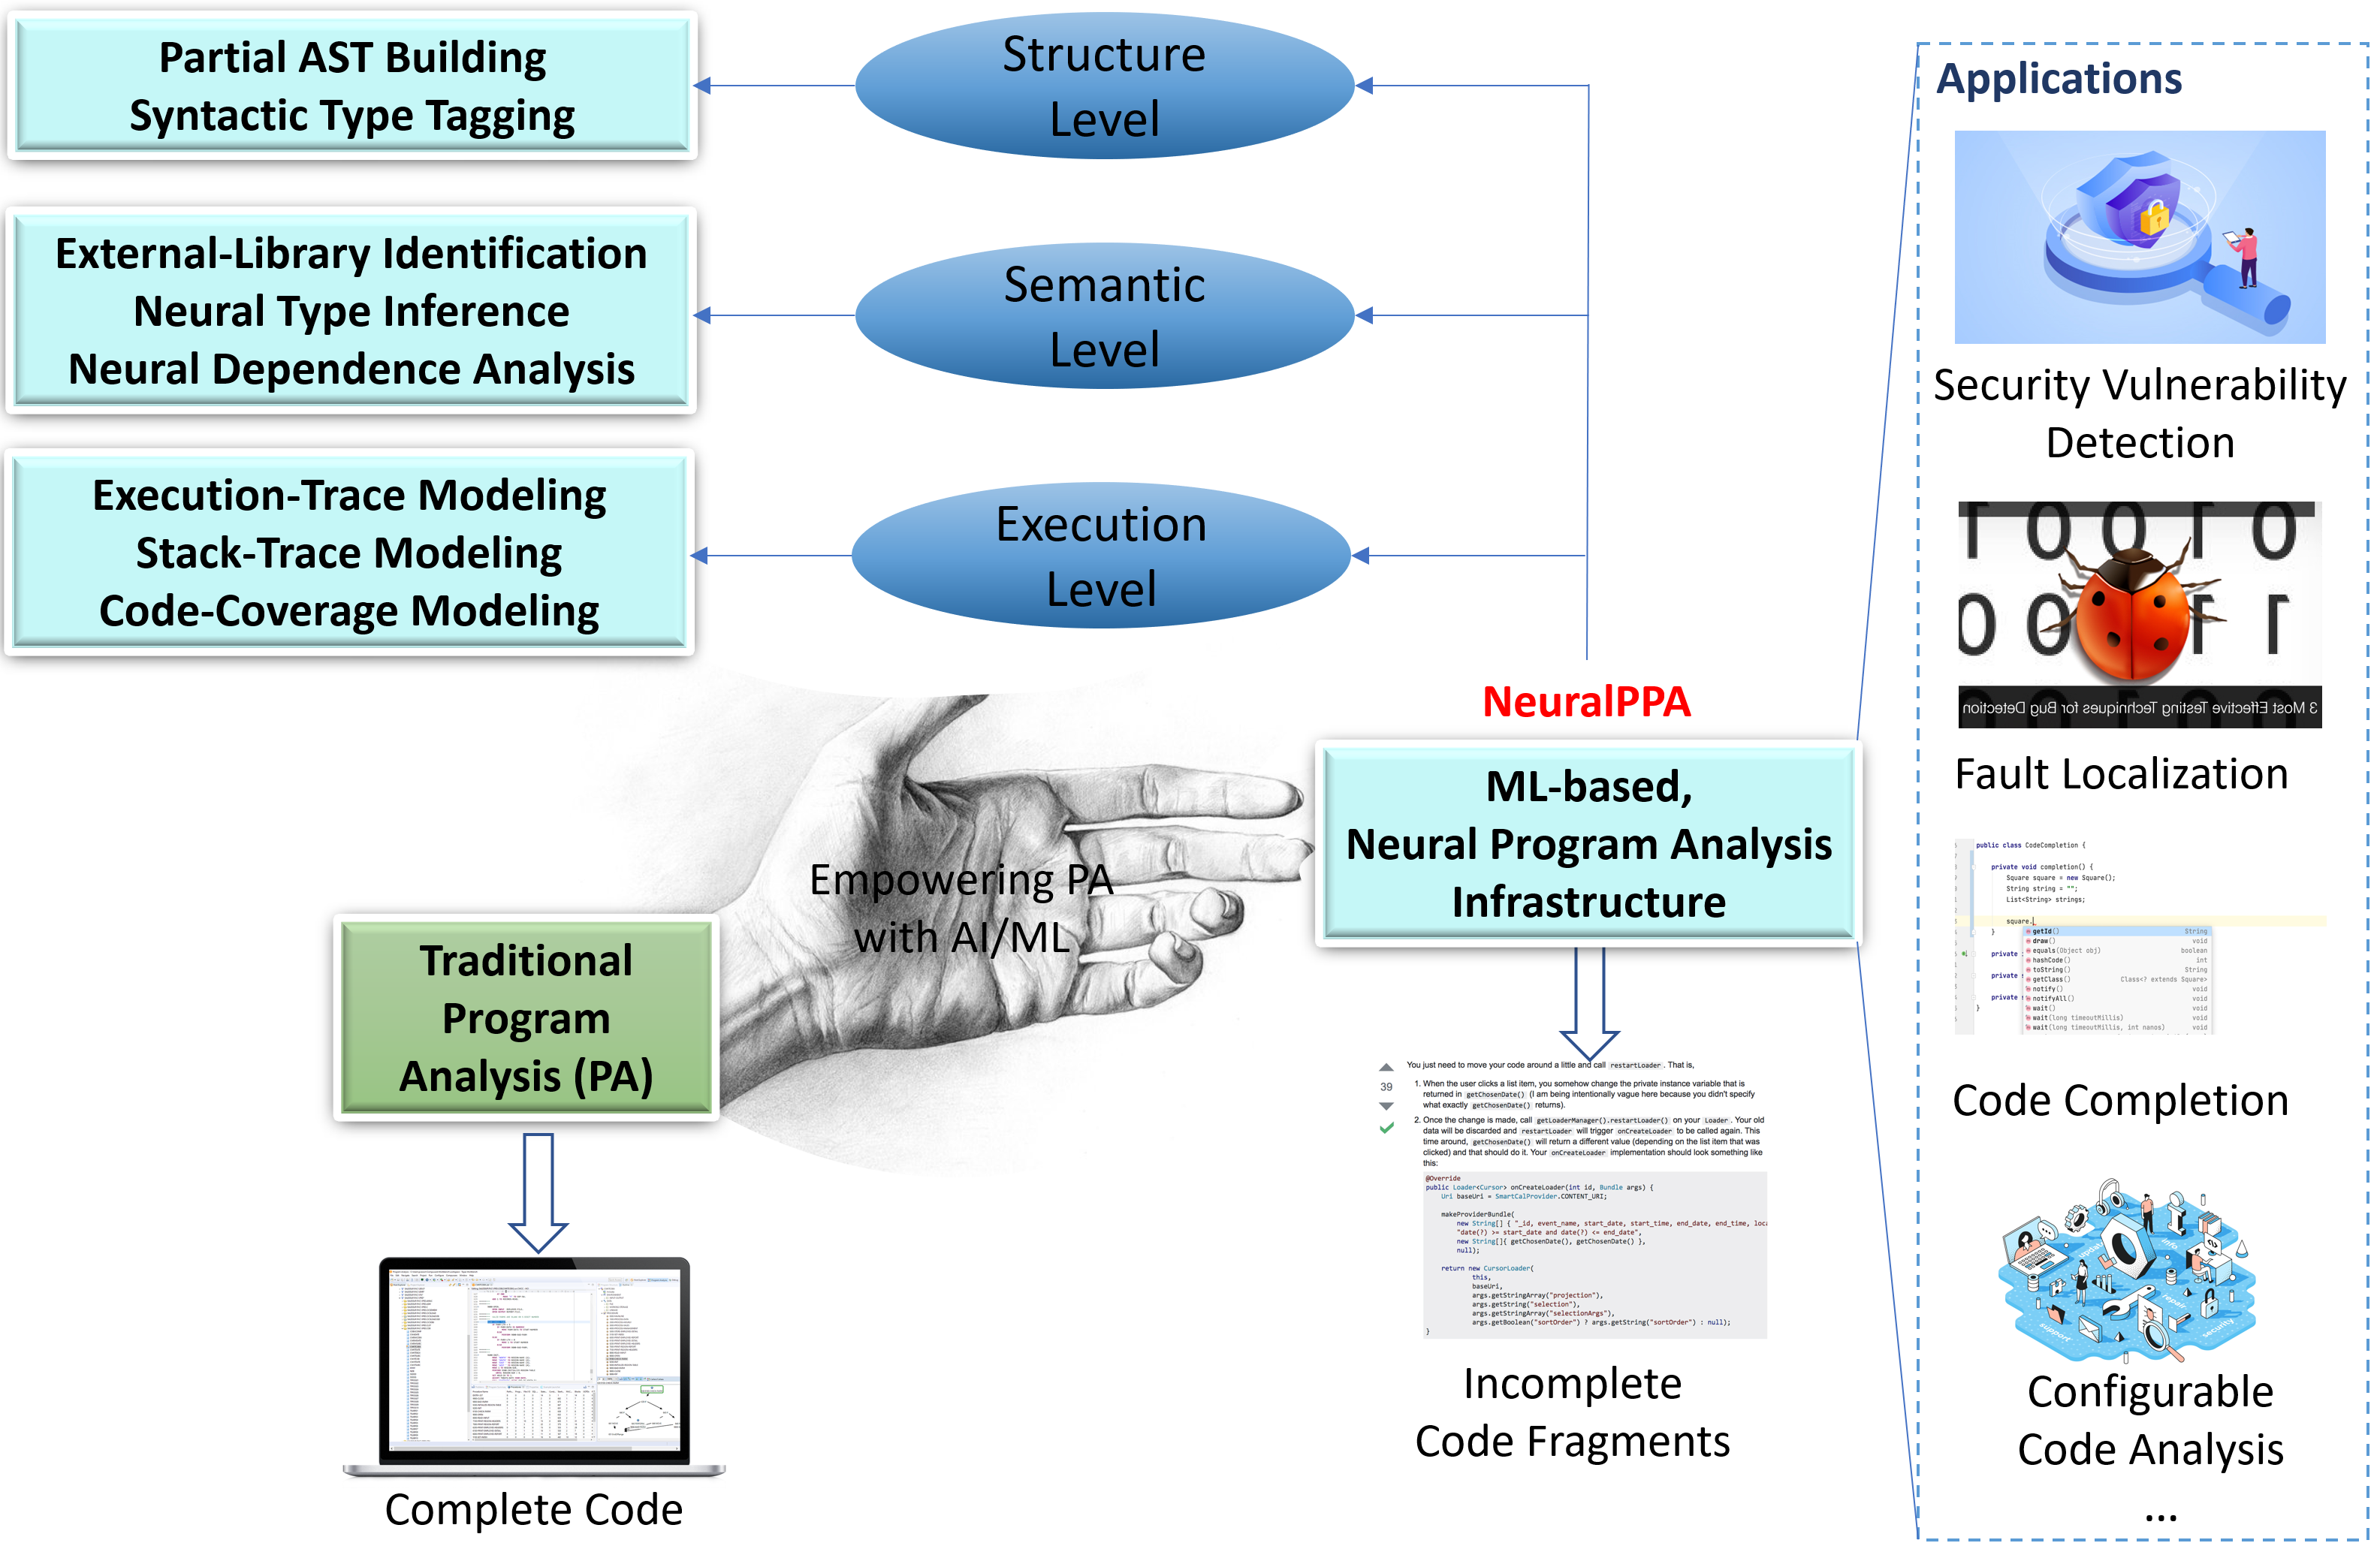
\includegraphics[width=0.83\textwidth]{graphs/neuralppa}
%    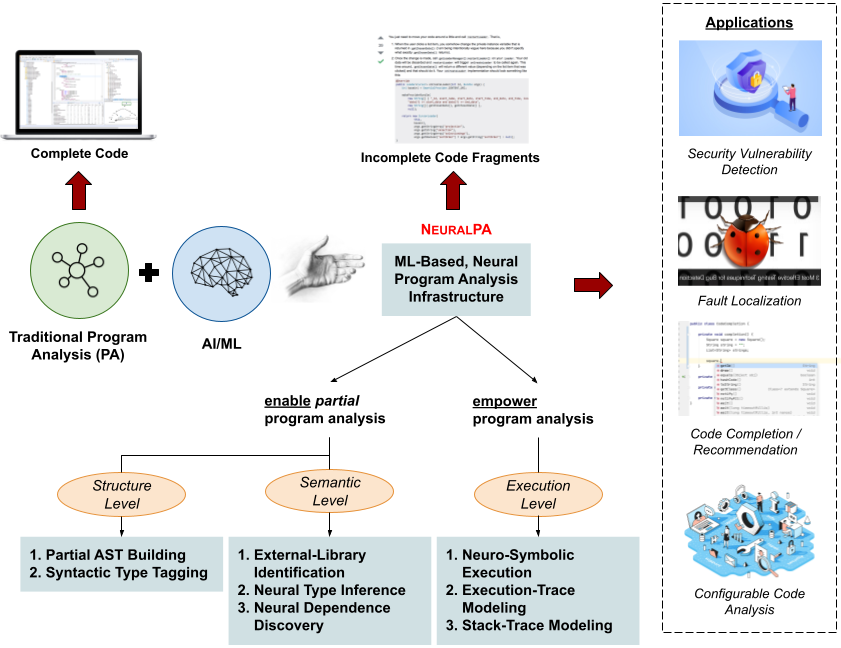
\includegraphics[width=0.92\textwidth]{figures/infra-design-3.png}
%    \vspace{-10pt}
%    \caption{{\tool}: Machine Learning-based Program Analysis Infrastructure}
%    \label{fig:arch}
%\end{figure}

In this proposal, we seek to create a paradigm shift in assisting the
visually-impaired programmers and learners with a Voice-to-Code
framework. We aim to establish {\em a scientific foundation, novel
  methodologies, frameworks, models, and algorithmic solutions for
  Voice-to-Code assistive technology}.

To address the above issues with the current assistive technology for
visually-impaired programmers and learners (VIPLs), we are embarking
on the development of a groundbreaking framework that leverages voice
interaction and advanced AI technologies.

{\bf Enabling Voice-Driven Interaction}: Our primary objective is to
empower visually-impaired programmers and students to interact
seamlessly with an IDE through the power of voice. This means that
instead of relying solely on audio cues, they will be able to
communicate their coding instructions and commands using spoken
language. By doing so, we aim to bridge the accessibility gap and
provide an intuitive and efficient way for visually-impaired
individuals to engage with programming tasks.

{\bf Voice-to-Text Conversion}: In our framework, the spoken word
becomes a bridge to the digital realm. We utilize state-of-the-art
voice recognition technology to accurately convert spoken language
into text. This initial step is crucial in translating the user's
voice commands and instructions into a format that can be further
processed by the system. This ensures that the users' intent is
accurately captured and preserved throughout the programming process.

{\bf Text-to-Code Generation with Generative AI}: Upon converting
voice inputs into textual form, we introduce the power of generative
artificial intelligence (AI). A large language model (LLM) with
generative capabilities takes the converted text and transforms it
into actual code. This step involves understanding the context,
syntax, and semantics of the instructions, and generating
corresponding code segments. The AI's ability to comprehend natural
language ensures that the generated code aligns with the user's
intentions.

{\bf Code Playback for Verification}: An integral aspect of our
framework is ensuring that the generated code is faithful to the
user's input. After the AI generates the code, it is read back to the
user through synthesized speech. This auditory feedback mechanism
enables visually-impaired programmers and students to verify the
accuracy of the generated code. By engaging their sense of hearing,
users can catch any discrepancies or errors and provide timely
corrections.

  
{\bf Empowering Modifications and Iterations}: Flexibility and control
are central to our framework's design. The visually-impaired users
have the ability to modify and refine the generated code according to
their preferences and needs. Through voice commands or text-based
interactions, they can make alterations, experiment with different
approaches, and fine-tune the code to align with their coding
goals. This iterative process ensures that the users are active
participants in the programming tasks.

In summary, our innovative framework for visually-impaired programmers
and learners offers a transformative way to engage with programming
tasks. By harnessing the capabilities of voice recognition, generative
AI from LLMs, and auditory feedback, we are working to create an
environment that fosters inclusivity, creativity, and
empowerment. Through this initiative, we aspire to break down barriers
and make the world of coding accessible to all, regardless of visual
impairments, contributing to a more diverse and vibrant programming
community.

\subsection{Thrusts of Research}

We propose the following thrusts of research in {\tool} (see Table~\ref{tab:milestones}):

\vspace{3pt}
%\noindent \textbf{Thrust 1. Neural Structural Analysis Infrastructure
%  \code{NeuralStruct}.} ({\em Section~\ref{}}) Source code has
%well-defined structures and semantics. Thus, the basic infrastructure
%in {\tool} is the neural structural analysis component.  This
%component has two main tasks. First, it learns from the syntactic
%structures of the complete code in the training dataset collected from
%large-scale code repositories, to derive the abstract syntax tree
%(AST) that best represents the syntactic structure of the given
%partial code, i.e., with the highest likelihood/probability.  The
%traditional lexical analyzer still works for partial code due to the
%independence nature of lexical tokens. The second task of this
%component is to tag the code tokens with the types of the syntactic
%units including the statement types (\code{if}, \code{for}, etc.),
%variables, fields, methods, classes, etc. Both of the tasks can be
%performed with our learning-based approaches in a dual-learning
%manner.

\noindent \textbf{Thrust 1. Empirical Study on Current Assistive
  Technology for VIPLs} ({\em Section~\ref{sec:thrust1}}) In order to
gain deeper insights into the challenges faced by visually-impaired
programmers and students in utilizing current assistive technologies
for programming or learning to program, we conducted an empirical
study. This study involved engaging a diverse group of
visually-impaired individuals with varying levels of programming
experience. Through in-depth interviews, surveys, and usability
testing, we aimed to uncover the specific pain points, limitations,
and usability issues encountered when utilizing existing assistive
tools in programming contexts. Participants were encouraged to share
their personal experiences, frustrations, and suggestions for
improvement. By systematically analyzing the data collected from this
study, we sought to identify common themes, technical obstacles, and
areas where assistive technologies fell short in meeting the unique
needs of visually-impaired individuals in the programming
domain. Ultimately, this empirical study serves as a foundational step
toward informing the development of more effective and inclusive
assistive technologies that cater to the diverse requirements of
visually-impaired programmers and students.



\vspace{3pt}
\noindent \textbf{Thrust 2. Voice-Driven Programming Framework for
  VIPLs.}  ({\em Section~\ref{sec:thrust2}}) Our initiative focuses on
empowering visually-impaired programmers and students by enabling them
to seamlessly interact with an integrated development environment
(IDE) through voice commands. Rather than relying solely on auditory
cues, this approach allows them to articulate coding instructions and
commands using spoken language, effectively bridging the accessibility
gap and providing an intuitive means for engaging with programming
tasks. Through cutting-edge voice recognition technology, spoken
language is converted into text, serving as a crucial initial step in
translating users' voice inputs into a processable format.

Subsequently, our framework integrates generative artificial
intelligence (AI) to facilitate the transformation of text back into
code. A sophisticated language model with generative capabilities
processes the textual input, considering the nuances of context,
syntax, and semantics to generate corresponding code segments that
accurately align with the users' intentions. To ensure the accuracy of
the generated code, our framework employs auditory feedback, where the
AI-generated code is read aloud to the user. This feedback mechanism
allows visually-impaired programmers and students to verify the code's
precision through their sense of hearing, enabling them to promptly
identify errors and discrepancies.

Central to our design is the empowerment of users through flexibility
and control. Visually-impaired individuals can actively modify and
refine the generated code to suit their preferences and coding
goals. This adaptability is facilitated through voice commands or
text-based interactions, allowing for alterations, experimentation
with diverse approaches, and fine-tuning of the code. This iterative
process ensures that users remain engaged and actively involved in the
programming tasks, ultimately fostering a sense of ownership and
inclusivity in their coding journey.

\vspace{3pt}
\noindent \textbf{Thrust 3. Voice-Driven Features for an IDE to
  support VIPLs.} ({\em Section~\ref{sec:thrust3}}) Introducing a
revolutionary programming environment tailored to the needs of
visually-impaired individuals, our cutting-edge platform offers a
multifaceted approach to programming through seamless voice
interaction. At the core of this environment lies direct communication
with ChatGPT, a sophisticated language model, which serves as a
personalized programming assistant. Users can articulate their
programming tasks through natural language voice commands, receiving
real-time feedback, suggestions, and guidance to navigate coding
challenges effectively. This feature not only democratizes the
programming experience but also empowers visually-impaired programmers
to engage in a more intuitive and productive coding process.

Our programming environment goes beyond voice interaction by enabling
the transformation of voice commands into tangible code. Leveraging
advanced voice recognition and generative AI technologies, users'
spoken instructions are converted into actual code snippets. This
bridges the gap between verbal expression and code creation, ensuring
that the users' intent is accurately translated into executable code
segments. The generated code is then read back to the users through
synthesized speech, allowing them to verify its accuracy and
completeness, while promoting a understanding of the
programming logic.

This innovative environment extends its functionality to seamlessly
integrate generated code with existing projects, simplifying the
collaborative process and enabling a cohesive workflow. In addition,
users can harness the power of voice to initiate debugging sessions,
identifying and rectifying errors through intuitive voice
commands. The environment also facilitates the generation of
comprehensive documentation, providing a holistic overview of the
codebase, which can be enriched and customized through voice
interactions. Furthermore, users can effortlessly create test cases
using voice commands, enhancing the testing and validation of their
code. By encompassing these features, our programming environment
empowers visually-impaired programmers with a versatile and inclusive
toolset, fostering a dynamic programming journey while mitigating
accessibility barriers.


%1) Voice interaction with ChatGPT on programming tasks

%2) Code Generation from Voice

%3) Reading back the generated code for verification

%4) Code integration with existing code

%5) Debugging code via Voice Commands

%6) Documentation generation

%7) Test case generation


%\vspace{3pt}
%\noindent \textbf{Thrust ???. Neural Execution Analysis Infrastructure.}
%({\em Section~\ref{}}) All the dynamic analysis techniques require the
%analysis and understanding of the execution. However, for an
%incomplete code, we first need to design a component that can wrap
%around the given code fragment with the minimum code so that the code
%fragment can be executed. When the code is executed, we also need the
%approaches that represent the executed statements and their relations,
%model the execution and stack traces, and model the code coverages
%for an execution.

\begin{table*}[t]
	\vspace{-15pt}
\begin{center}
{\footnotesize{
\begin{tabular}{cc}
\begin{tabular}[t]{|p{0.2in}|p{2.95in}|} 
\hline
\multicolumn{2}{|>{\columncolor[gray]{0}}c|}{\textcolor{white}
{\bf Year 1 Project Milestones \& Deliverables}}\\
\hline 
\hline
\multicolumn{2}{|c|}{\bf T1. Neural Structure Analysis Infrastructure}\\
\hline
{\bf 1.1} & Neural Syntactic Type Tagging\\
{\bf 1.2} & Neural Partial AST Building\\
{\bf 1.3} & Evaluation of the components\\
\hline
\hline
\multicolumn{2}{|c|}{\bf T2. Neural Semantic Analysis Infrastructure}\\ 
\hline
{\bf 2.1} & External-Library Identification\\
\hline
%\hline
%\multicolumn{2}{|c|}{\bf Integrate Code Synthesis into Tools}\\
%\hline
%{\bf 1.5} & \goalOneFour.\\
%\hline
\multicolumn{2}{c}{}
\end{tabular}
&
\begin{tabular}[t]{|p{0.2in}|p{2.95in}|} \hline
\multicolumn{2}{|>{\columncolor[gray]{0}}c|}{\textcolor{white}
{\bf Year 2 Project Milestones \& Deliverables}}\\
\hline 
\hline
\multicolumn{2}{|c|}{\bf T2. Neural Semantic Analysis Infrastructure}\\
\hline
{\bf 2.2} & Neural Type Inference\\
{\bf 2.3} & Neural Dependence Analysis\\
%{\bf 2.3} & Integrate Evaluation Framework into Design Environment\\
%{\bf 2.4} & Evaluate CRL Framework with Existing Models\\
%{\bf 2.3} & \goalTwoThree.\\

\hline
\hline
\multicolumn{2}{|c|}{\bf T3. Neural Execution Analysis}\\ 
\hline
%{\bf 3.1} & Design New Code Representations and Learning Models.\\
{\bf 3.1} & Neural Execution-Trace Modeling\\
%{\bf 2.4} & Advance FL and RT-CI Approaches.\\
%{\bf 2.5} & Advance Regression Testing in CI Approaches.\\
%{\bf 2.5} & Advance APR Approaches with Framework.\\
\hline
%\hline
%\multicolumn{2}{|c|}{\bf Community Involvement: Capacity Building}\\
%\hline
%{\bf 2.4} & \goalTwoFour.\\
%{\bf 2.5} & \goalTwoFive.\\
%{\bf 2.6} & \goalTwoSix.\\
%\hline
\multicolumn{2}{c}{}
\end{tabular}
\end{tabular}\\
\vspace*{-.3cm}
\begin{tabular}{c}\hline
\multicolumn{1}{|>{\centering\columncolor[gray]{0}}p{6.44in}|}{\textcolor{white}
{\bf Year 3 Project Milestones \& Deliverables}}\\
\hline
\end{tabular}\\
\vspace*{-.2cm}
\begin{tabular}{cc}
\begin{tabular}[t]{|p{0.2in}|p{2.95in}|}
\hline
\multicolumn{2}{|c|}{\bf T3. Neural Execution Analysis}\\
\hline
{\bf 3.2} & Neural Stack Trace Modeling\\
{\bf 3.3} & Neural Code Coverage Modeling\\

%{\bf 3.3} & Testing on Models in IDE tools.\\
\hline
%\hline
%\multicolumn{2}{|c|}{\bf \goalTwo}\\ 
%\hline
%{\bf 3.3} & \goalThreeThree.\\
%\hline
\multicolumn{2}{c}{}
\end{tabular}
&
\begin{tabular}[t]{|p{0.2in}|p{2.95in}|}
\hline
\multicolumn{2}{|c|}{\bf T4. Neural Partial Program Analysis Applications}\\
\hline
%{\bf 3.1} & Design New Code Representations\\

{\bf 4.1} & Security Vulnerablity Detection with {\tool}\\
{\bf 4.2} & Fault Localization and Completion with {\tool}\\

\hline
\multicolumn{2}{c}{}
\end{tabular}
\end{tabular}
\vspace{-15pt}
}}
\end{center}
\vspace*{-.3in}
%\caption{Tasks and Milestones. (Rep. = Representation)}
\caption{The 3-year schedule of Thrusts, Tasks, and Milestones of this proposal.}
%the schedule of Thrusts, Tasks, and Milestones of this proposal.
%\vspace{-10pt}
\label{tab:milestones}
\vspace{-10pt}
\end{table*}
%




%\subsection{Significance of This Proposed Project: NSF Merit Criteria}

\section{Intellectual Merits}

The results of this project will advance the state-of-the-art
knowledge and scientific foundations in AI/ML for Software
Engineering. They are transformative and directly help improve
software engineering tools empowered by AI/ML.

\noindent \underline{{\bf Advance the state-of-the-art knowledge and
    understanding}}. Voice-driven programming framework will advance
the body of knowledge and theoretical foundations for machine learning
and AI for code. The empirical study in Thrust 1 will help advance the
state-of-the-knowledge in how assistive technology for VIPLs should
be.

\noindent \underline{{\bf Scientific foundation, creative/original
    research}}. This project will provide a scientific foundation
(novel concepts, representations, algorithms, models, and tools) (1)
to enable voice-driven assistive technology, (2) to advance the AI/ML
models in both voice recognition and code generation, and (3) to
enable the applications of AI/ML for code research in building
interactive IDEs for VIPLs.

\section{Broader Impacts}

\underline{{\bf (1) Transformative and benefits to society}}. our
programming environment empowers visually-impaired programmers with a
versatile and inclusive toolset, fostering a dynamic programming
journey while mitigating accessibility barriers. We aspire to break
down barriers and make the world of programming accessible to all,
regardless of visual impairments, contributing to a more diverse and
vibrant programming community.


\noindent\underline{{\bf (2) Foster other related research
    activities}}. Our results will foster {\em research activities in
  related fields of {\bf machine learning} and {\bf software
    engineering}}. We will produce theoretical concepts and techniques
that are novel in deep learning, e.g., novel neural networks to model
and learn for code.

%The applications of our neural program analysis in software
%engineering applications will advance software security and
%reliability.

\noindent\underline{{\bf (3) Education, dissemination, and broader
    participation}} (Section~\ref{edu}). The research will enhance the
infrastructure for teaching/research via tools and data sets for use
by students and practitioners, and for enhancement by researchers. We
will provide related learning modules for educators as well. It will
include outreach activities for undergraduate students,
underrepresented groups, minorities, and women in science.

\section{Related Work}
\label{sec:related}

A rich body of literature describes accessibility tools
designed for VIPLs, and many of them have been
tested in diverse
environments~\cite{10.1145/1056808.1057018,10.1145/800071.802260,10.1006/jnca.1998.0060,10.1145/2501988.2502047,10.1145/568600.568611,10.1145/3308561.3354616,10.1145/1168987.1169035,10.1145/1408760.1408761,10.1145/238386.238405,10.5555/1103141.1103147,10.1145/1953163.1953323,5306335,10.1145/1121341.1121427,10.1145/2889160.2889188,10.1145/2889160.2891041,10.1145/3132525.3132550,10.1145/3170427.3188696,10.1145/2661334.2661385,10.1145/292834.292839,10.1145/563517.563372,10.1145/2556288.2557073,5967168,10.1145/1029014.1028654,10.1145/354324.354356,4268242,10.1016/j.ijhcs.2011.07.002,10.1145/1953163.1953323,10.1145/2982142.2982168,casten2005knowledge,CHIANG2005394,crossland2014smartphone,10.1145/1357054.1357250,gill2013digital,horowitz2003influence,10.1145/274497.274512,10.1145/354324.354327,janiszewski2006low,10.1145/1639642.1639663,margrain2000helping,massof2002model,massof2002model,scott2002impact,theofanos2005helping,watson1997national,falase2019tactile,10.1145/3480169,9833098,10.1145/3517428.3544806,10.1145/3449203,10.1145/3526113.3545620,10.1145/3517428.3544812,10.1145/3526114.3558649,9240634,10.1145/3507469,10.1145/3178412.3178414,10.1145/3373625.3417998,10.1145/3441852.3471221,7522265,10.1145/3550356.3561591,10.1145/3555609,10.1145/3561391,10.1145/3585315,su12135320,8783291,Matti2017PreservingTS,10.1145/3526114.3558641,10.1145/2533682.2533683,10.1145/3392063.3394437,Morrison2018TorinoAT,Pires2020ExploringAP,Pires2023TACTOPIEP,Mountapmbeme2022AddressingAB,Kim2023TangiblePL,Schanzer2019AccessibleAP,Schanzer2020AdaptingSI,Wang2023VirtualSC,Stefik2019ComputerSP,Ladner2020ComputerSP,Strassman2019TeachingAL,Mountapmbeme2021HowTO,Kim2022DevelopmentOT,AlOtaibi2020TeachingPT,Kapucu2022ExploringCS,Koehler2019StudentsWV,Akarsu2022AnIT,Kzlaslan2019AHC,Kzlaslan2020ImproveLW,Tsinajinie2020AnOP,2023IMPROVINGSP,Milne2018Blocks4AllOA,Villar2019PhysicalPF,Rocha2021AccemblyAH,Rocha2023CodingTO}. However,
none of them addresses the aforementioned issues with generative AI and Large Language Models in Voice-to-Text and Text-to-Code as
in our proposal.

{\bf Research on the programming experiences of VIPLs} is notably
lacking, both in terms of quantity and quality. Mealin and Murphy-Hill
conducted qualitative interviews~\cite{mealin-vlhcc12} with eight experienced blind
developers and discovered several noteworthy insights. Although some
of these developers had utilized popular IDEs, e.g., Eclipse and
Visual Studio, they primarily relied on text editors for their coding
tasks. Interestingly, the interviewees indicated a tendency to switch
between different editors or IDEs based on the specific demands of
their projects. This behavior suggests that certain aspects of IDEs
are indeed useful and practical for blind programmers. However, the
overall inaccessibility of these environments often discouraged them
from using them over alternative tools.
%This discovery strongly underscores the need for concerted efforts to
%make IDEs more accessible and inclusive for this community.
Furthermore, the study revealed that these developers either refrained
from using or rarely engaged with the tools and features provided
within the IDEs.
%The precise reasons for this behavior were not
%conclusively determined, and
The study proposed several potential hypotheses. These included the
challenges associated with navigating the user interfaces of IDEs or
the complexities involved in setting up these tools. This gap in
research can be attributed to the study's methodology, which relied on
qualitative interviews with a predetermined set of questions. While
this approach helped surface the most pressing issues as reported by
the developers themselves, it fell short in uncovering the underlying
causes of these problems, as the interviewees did not possess these
answers.
%Consequently, when conducting research with specialized user groups such as visually impaired individuals, it is imperative to meticulously design the research methodology to not only gather valuable insights but also address the "why" questions.
Mealin and Murphy-Hill's study~\cite{mealin-vlhcc12} also yielded valuable insights into
the primary challenges faced by blind software developers, including
(1) difficulties in gaining an overview of the code, whether their own
or someone else's; (2) challenges in searching for information within
the code; and (3) struggles with accessing the tool library and
discovering tools within the IDEs. These points serve as valuable
inspiration for the development of tools and products aimed at
enhancing the productivity of VIPLs.

In a parallel study, Albusays and Ludi conducted a quantitative survey~\cite{khaled16} involving 69 experienced blind programmers who self-reported their experiences working on programming projects. Their findings reinforced the challenges outlined by Mealin and Murphy-Hill~\cite{mealin-vlhcc12}. These developers encountered considerable difficulties in navigating through complex code structures and layouts. Additionally, some respondents expressed discomfort and hesitancy when seeking assistance from or collaborating with sighted fellow developers. In addition to these new findings, Albusays and Ludi's research echoed the shared observation of the lack of accessibility in IDEs and their tools for visually impaired users.

%Both studies, however, encountered a common limitation in their inability to uncover comprehensive explanations for this inaccessibility, a limitation stemming from their reliance on respondent-dependent research methodologies.

%============================

{\bf Accessible and assistive tools for visually impaired developers}.
Stefik {\em et al.} introduced Sodbeans~\cite{stefik11}, an auditory
integrated development environment (IDE) that employs audio cues to
convey information about code to developers. A notable feature of
Sodbeans is its utilization of scoping cues, which signify
relationships between program constructs.
%For instance, numerical values like "1 nested loop" denote different
%levels of loops. Testing with users revealed that scoping cues enhance
%code comprehension uniformly across various experience levels of
%sighted programmers, with no adverse effects.
However, Sodbeans primarily focuses on improving code comprehension,
with its potential to address the primary issue identified by Mealin
and Murphy-Hill ~\cite{mealin-vlhcc12} – gaining an overview of code – considered a
secondary goal necessitating further trials with non-sighted
developers for verification. Sodbeans was later integrated into
Oracle's Netbeans as an IDE extension.

Before their work on Sodbeans IDE, Stefik {\em et al.} created the
Wicked Audio Debugger (WAD)~\cite{wad07}, an audio-based add-in debugger for
Microsoft Visual Studio in 2007. WAD aimed to assist blind developers
in code navigation and debugging, potentially saving time and effort
in bug identification and resolution. However, feasibility testing
involved ten sighted senior-level computer science students simulating
"blind" behavior without visual code access or prior structural
knowledge. Similar to the study~\cite{stefik11} on Sodbeans, the
positive impact on blind developers' productivity remained
inconclusive.

Similarly addressing this challenge, Baker {\em et al.} developed a
plug-in called StructJumper~\cite{BakerML15} for Eclipse to aid
visually impaired developers in comprehending and navigating code. The
plug-in comprises two main features, TreeView and Text Editor,
creating a hierarchical tree based on Java's nesting
structure. Effectiveness tests conducted with seven experienced blind
programmers showed a slight positive impact on task completion time.
%As of May 2023, no updated versions of StructJumper are publicly available on the internet.
However, being an Eclipse plug-in limits its accessibility for many blind programmers, as they must switch between different IDEs with exclusive assistive tools and plug-ins.

Although each of these three initiatives can provide valuable support
to blind software developers, they currently exist as separate
entities integrated into different IDEs (Netbeans, Eclipse, and Visual
Studio).

Armaly and McMillan~\cite{armaly-tse18} performed a study on program
comprehension strategies by blind and sighted
programmers. AudioHighlight~\cite{armaly-icsme18} renders the code
inside a web view and places HTML heading tags on the structural
elements of a source file such as classes, functions and control flow
statements. 

%This necessitates developers to install and use all three
%IDEs simultaneously and correctly incorporate the respective plug-ins,
%creating a time-consuming and demotivating barrier for visually
%impaired programmers seeking to optimize their work environment.
%Furthermore, these tools were designed primarily for experienced blind
%programmers rather than beginners, as evident from the selection of
%testers, who were either professionally trained in computer science or
%had years of experience in the field.
%Insights gathered from these initiatives may differ significantly from
%those of beginners just embarking on their programming.

%Despite prior efforts to understand the challenges faced by blind software developers and create supportive tools, numerous gaps remain that can be addressed to better serve this unique group of learners and workers. This study introduces Product P4H with the aim of addressing the four major gaps identified through an analysis of existing work:

%Our ongoing effort in an empirical study include (1) uncovering
%obstacles hindering the pursuit of programming education by the
%general blind population, (2) addressing the needs of novice
%programmers, (3) conducting user research to comprehensively
%understand the challenges faced by blind programmers, and (4)
%eliminating the fragmentation of existing solutions. The fifth gap,
%feasibility testing with a suitable user group (inexperienced blind
%programmers), is partially addressed through the integration of a data
%tracking system within the product. However, further steps to fully
%address this fifth gap will be discussed in the limitations and future
%work section.





%\section{\color{red}{Related Work}}
%Our project is closely related to the following research literature: 
\textbf{Code Representation Learning (CRL).}  The recent success in
machine learning has lead to strong interests in applying machine
learning, especially deep learning, to programming language (PL) and
software engineering (SE) tasks, such as automated correction for
syntax errors~\cite{Bhatia-2016}, fuzz testing~\cite{Patra-2016},
program synthesis~\cite{Amodio-2017}, code
clones~\cite{White-2016,Smith-2009,Li-2017}, program
summarization~\cite{Allamanis-2016,Mou-2014}, code
similarity~\cite{Zhao-2018,Alon-2018}, probabilistic model for
code~\cite{Bielik-2016}, and path-based code representation,
e.g., Code2Vec~\cite{Alon-2018} and Code2Seq~\cite{alon2018code2seq}. 

%In the above PL and SE tasks, 
%All approaches learn code
%representations using different program properties. 
%Although not proposed for detecting bugs, they
%still very relevant to our proposal. %as one important step of our approach is to learn bug detection specialized code representation.

%Different from the existing CRL approaches, in our initial
%study~\cite{yioopsla19}, we conducted the CRL using the AST, DFG, PDG,
%and different attention-based neural networks. Our results show that
%our CRL is more suitable for detecting bugs than the existing baselines.


\textbf{Bug Detection.}
%Many techniques have been developed for rule-based and learning-based bug detection. 
Some existing rule-based bug detection approaches,
such as
\cite{Bian-2018,Jin-2012,Olivo-2015,Engler-2001,Cole-2006,Toman-2017},
are unsupervised. However, new rules are needed to
define to detect new types of bugs, e.g., FindBugs~\cite{Hovemeyer-2007} and NAR-miner~\cite{Bian-2018}.
%
%The most state-of-the-art \textit{rule-based} tool is NAR-miner~\cite{Bian-2018} that extracts
%negative code rules to detect bugs. %, instead of positive code rules. 
%Our initial results show the NAR-miner has a
%high false positive rate, i.e., 52\%, which make them
%impractical for daily use. 
%that it only costs NAR-miner 1 minute to perform bug detection on
%a project. However the mining-based approaches mainly suffer the
%problem of high false positive (FP) rates, such as the NAR-miner has a
%high FP rate, i.e., 52\% in the cross-project setting, which make them
%impractical for daily use. 
%When comparing our approach with the existing state-of-the art rule-based and mining approaches, the main differences are as follows. First, we consider the relations among paths from different methods for detecting cross-method bugs. However,
%they normally work on individual methods and cannot work well on the
%cross-method bugs. Second, our approach covers path information in an
%AST in order to detect very detailed bugs in each method, while the
%they often consider the important rules and may miss some information
%outside of their rules.
To overcome the pre-defined rules, the mining-based approaches, e.g.,~\cite{Bian-2018,Jin-2012,Olivo-2015,Engler-2001,Cole-2006,Toman-2017,Li-2005}, were proposed to mine implicitly programming rules from source code using data mining techniques. 
%Typically, this type
%of approaches extracts implicitly programming
%rules from program source code using data mining approaches
%(e.g., mining frequent itemsets or sub-graphs) and detects
%violations of the extracted rules as potential bugs. 
They still have a key limitation in a very high false positive rate
due to the fact that they cannot distinguish the cases of incorrect
code versus infrequent/rare code.  There exist DL-based
approaches~\cite{Pradel-2018,Wang-2016b} and traditional ML
techniques~\cite{Engler-2001,Li-2005,Wasylkowski-2017,
  Wang-2016b,Wang-2016,Liang-2016}.
%For example, 
%the Bugram \cite{Wang-2016} uses n-gram models to rank the methods and then picks the top-ranked methods as buggy methods.
%DeepBugs~\cite{Pradel-2018} uses deep learning techniques to propose
%a name-based bug detector.  
DL-based approaches are still limited to detect bugs in individual
methods.
%without investigating the dependencies among different yet
%relevant methods.

%$Due to that, they have high false positive rates, making them less
%practical in the daily use of software developers.
%In practice,
%there exist several cases that bugs occur across more than one
%method. That is, to decide whether a given method is buggy or not, a model
%needs to consider other methods that have data and/or control
%dependencies with the method under investigation. 
%Due to that, the
%existing DL-based approaches have high false positive
%rates, making them less practical in the daily use. % of software
%developers. 
%For example, DeepBugs~\cite{Pradel-2018} is reported to have a high false positive rate of 32\%. That is, approximately one out of 3 reported bugs is not a true bug, thus, wasting much developers' efforts. 
%Our study~\cite{yioopsla19i} also showed a false positive rate of 41\% for DeepBugs on our collected dataset.


%In this paper, our approach is also using the deep learning techniques to train the models and
%classify methods into buggy or non-buggy. Our approach is different
%from the existing learning-based approaches in the following ways.
%First, like the rule-based approaches, the existing learning-based
%approaches do not consider the relations among paths across multiple
%methods. In our code representation learning step, we model the
%relations among paths from different methods using the dependencies of
%entities in the PDG and DFG, in addition to the AST nodes of a path.
%Second, our approach uses long paths of an AST to cover all of the AST
%nodes for representing local context, while other existing approaches
%often use part of method information to detect bugs, such as
%name-based identifier representation and frequent $n$-grams. Our
%results show that our approach can outperform all of the
%studied baselines.


%\textit{Machine learning-based bug	detection~\cite{Wasylkowski-2017,Wang-2016b,Wang-2016,Pradel-2018}.}
%With the advances of machine learning (ML) and especially deep
%learning models, several approaches have been proposed to learn from
%previously known and reported bugs and fixes to detect bugs in the
%new code. While the ML-based bug detection models~\cite{Nam-2015}
%rely on feature selections, the deep learning-based
%ones~\cite{Pradel-2018,Wang-2016b} take advantages of the capability
%to learn the important features from the training data for bug
%detection. 


\textbf{Fault Localization and Regression Testing.}
Spectrum-based Fault Localization (SBFL)~\cite{zhang2011localizing, abreu2007accuracy, jones2005empirical, abreu2006evaluation, naish2011model, wong2007effective, liblit2005scalable, lucia2014extended, keller2017critical} has been intensively studied in the literature, e.g., Ochiai \cite{abreu2006evaluation} and Jaccard \cite{abreu2007accuracy}. 
%Tarantula \cite{jones2001visualization}, SBI \cite{liblit2005scalable}, Ochiai \cite{abreu2006evaluation} and Jaccard \cite{abreu2007accuracy}.  
%they share the same basic insight, i.e., code elements mainly executed by failed tests are more suspicious. 
Mutation-based Fault Localization (MBFL)~\cite{moon2014ask, zhang2013injecting,budd1981mutation, zhang2010test, musco2017large} aims to additionally consider impact information for fault localization, e.g., Metallaxis \cite{papadakis2012using, papadakis2015metallaxis} and MUSE \cite{moon2014ask}.
%Since code elements covered by failed/passed tests may not have any impact on the corresponding test outcomes, e.g., Metallaxis \cite{papadakis2012using, papadakis2015metallaxis} and MUSE \cite{moon2014ask}.
%typical MBFL techniques
%use mutation testing \cite{budd1981mutation, zhang2010test, musco2017large} to simulate the impact of each
%code element for more precise fault localization, e.g., Metallaxis \cite{papadakis2012using, papadakis2015metallaxis} and MUSE \cite{moon2014ask}.
%The first general MBFL technique, Metallaxis [24, 26] is based on the
%following intuition: if one mutant has impacts on failed tests (e.g.,
%the tests outcomes change after mutation), its corresponding code
%element may have caused the test failures
%
%The more recent MUSE [23] technique has similar insights: (1)
%mutating faulty elements may cause more failed tests to pass than
%mutating correct elements; (2) mutating correct elements may
%cause more passed tests to fail than mutating faulty elements.
%
%Learning-to-Rank (LtR) has been used to improve fault localization~\cite{b2016learning, xuan2014learning, li2017transforming, sohn2017fluccs}.
%MULTRIC \cite{xuan2014learning} combines different suspiciousness values from SBFL. Some work combines SBFL suspiciousness values with
%other information, e.g., program invariant \cite{b2016learning} and source code complexity information \cite{sohn2017fluccs}, for more effective LtR fault localization. 
%TraPT \cite{li2017transforming} combines suspiciousness values from both SBFL and MBFL. 
Neural networks have been applied to fault
localization~\cite{zheng2016fault, briand2007using, zhang2017deep,
  wong2009bp}. However, they mainly work on the test coverage
information, which has clear limitations (e.g., it cannot distinguish
elements accidentally executed by failed tests and the actual faulty
elements)~\cite{li2017transforming}. DeepFL~\cite{DeepFL},
deep-learning based, was proposed to improve method-level FL, and it
improves the learning-to-rank FL approach,
TraPT~\cite{TraPT}. Extensive research has been on test case selection and prioritization in regression testing (RT), e.g., coverage-based~\cite{di2015coverage}, search-based~\cite{de2011multi,yu2010time}, historical tests~\cite{kim2002history,marijan2013test,noor2015similarity,park2008historical}, code dependencies~\cite{gligoric2015ekstazi} and information retrieval~\cite{kwon2014test,saha2015information}. 
%RT in Continuous Integration (CI) differs from the traditional RT as 
However, most techniques cannot be applied at the scale of modern Continuous Integration (CI) practices~\cite{elbaum2014techniques} that require frequent commits to the shared code base and cause the cost of continuous RT escalate dramatically~\cite{memon2017taming}. For example, coverage information may be infeasible and imprecise to collect at large scale and in quick cycles and code changes~\cite{elbaum2014techniques,haghighatkhah2018test,hemmati2015prioritizing,yu2018study}. 
Recently, RT in CI has been investigated, e.g.,~\cite{elbaum2014techniques,gligoric2015practical,yu2018study,jiang2009adaptive,henard2016comparing}. 
However, existing approaches, e.g.,~\cite{bertolino2020learning,spieker2017reinforcement} are still limited in accuracy and scalability as they lack the learning of deep features of test cases and source code and their relations. 
%Moreover, very little research has been devoted to investigating deep learning for RT in CI. 


\textbf{Automated Program Repair.}
%The earlier approaches for automated program repair (APR) aim to derive {\em similar fixes for similar source code}. Ray and Kim~\cite{ray-fse12} automatically detect similar fixes for similar code that are ported or branched out. FixWizard~\cite{icse10} automatically derives {\em the fixes for similar code} that were cloned from one place to another.
APR approaches have explored search-based SE to tackle more general
types of bugs, e.g., GenProg~\cite{le2011genprog},
RSRepair~\cite{qi2014strength}, MutRepair~\cite{martinez2016astor},
PAR~\cite{kim2013automatic}, and SPR~\cite{long2015staged}.
%\cite{le2011genprog,qi2014strength,LeGoues-icse12,martinez2016astor}.
%A search strategy is performed in the space of potential solutions
%produced by several operators that mutate the buggy code. Then, the
%test cases and/or program verification are applied to select the
%better candidate fixes~\cite{smith2015cure}. 
%Smith et al.~\cite{smith2015cure} showed that 
%However, these
%approaches tend to overfit on test cases, by generating incorrect
%patches that pass the test cases, mostly by deleting functionalities~\cite{smith2015cure}.
%
%GenProg~\cite{le2011genprog} uses genetic search on repair mutations
%and works at statement-level by inserting, removing or replacing a
%statement taken from other parts of the same
%program. RSRepair~\cite{qi2014strength} fixes buggy programs with
%random search to guide the patch generation
%process. MutRepair~\cite{martinez2016astor} attempts to generate
%patches by applying mutation operators on suspicious if-condition
%statements. 
%PAR~\cite{kim2013automatic} is based on {\bf fixing templates} that
%were manually extracted from 60,000 human-written patches. 
%Later
%studies (e.g., \cite{le2016history}) showed that the six templates in PAR~\cite{kim2013automatic} could fix only a few bugs in Defects4J. 
%Anti-patterns were integrated into search-based APR tools~\cite{tan2016anti}
%Anti-patterns were integrated into search-based APR tools, e.g., GenProg~\cite{le2011genprog} and SPR~\cite{long2015staged}), to help alleviate the problem of incorrect or incomplete fixes.
%Theses search-based approaches rely much on the quality of mutation operations and the fixing patterns.
%
%\textbf{Hard-coded Rules based APR.}  Some existing APR techniques are
%mostly based on hard-coded rules and operators, defined by human
%experts, used to generate potential patches obtained with mutation
%operators for a buggy code.  For example, GenProg~\cite{le2011genprog}
%uses genetic search on repair mutations and works at statement-level
%by inserting, removing or replacing a statement taken from other parts
%of the same program.  RSRepair~\cite{qi2014strength} tries to fix
%buggy programs with the same mutation operations in GenProg but uses
%random search to guide the patch generation process.
%MutRepair~\cite{martinez2016astor} attempts to generate patches by
%applying mutation operators on suspicious if-condition statements.
%These approaches have several limitations, rooted in the fact that
%they are based on handcrafted rules with limited scope (i.e., single
%statements, limited number of mutation operators, specific parts of
%expressions).  Moreover, Smith et al.~\cite{smith2015cure} showed that
%these approaches tend to overfit on test cases, by generating
%incorrect patches that pass the test cases, mostly by deleting
%functionalities.
%
%Kim et al.~\cite{kim2013automatic} initiated with PAR a milestone of APR based on fix templates that were manually extracted from 60,000 human-written patches. Later studies (e.g., \cite{le2016history}) have shown that the six templates used by PAR could fix only a few bugs in Defects4J.
%~\cite{tan2016anti} manually define a set of patterns for patch generating or filtering based on repair history.
%Anti-pattern~\cite{tan2016anti} integrated anti-patterns into two existing
%search-based automated program repair tools (namely, GenProg~\cite{le2011genprog} and SPR~\cite{long2015staged}) to help alleviate the problem of incorrect or incomplete fixes resulting from program repair.
%In their study, the anti-patterns are defined by themselves and limited
%to the control flow graph. Additionally, their anti-patterns are
%not meant to solve the problem of deriving better patches
%automatically, provide more precise repair hints to developers.
%In contrast to search-based approaches, other approaches have aimed to
%Another type of APR approaches {\bf mine and learn fixing patterns} from prior bug
%fixes~\cite{nguyen2013semfix,le2016history,liu2019avatar,kim2013automatic}, \textit{generating the state-of-the-art performance}. 
Another type of APR approaches {\bf mine and learn fixing patterns} from prior bug
fixes, \textit{generating the state-of-the-art performance}. The fixing patterns (or namely fixing templates) could be automatically
or semi-automatically mined, such as SemFix~\cite{nguyen2013semfix}, Prophet~\cite{long2016automatic}, Genesis~\cite{long2017automatic}, FixMiner~\cite{koyuncu2018fixminer}, HDRepair~\cite{le2016history}, CapGen~\cite{wen2018context}, SimFix~\cite{jiang2018shaping}, Avatar~\cite{liu2019avatar}, Nopol~\cite{Nopol}, ACS~\cite{ACS}, SketchFix~\cite{SketchFix}, ELIXIR~\cite{saha2017elixir}, and LSRepair~\cite{LSRepair}. Tbar~\cite{tbar-issta19} collects all existing fix-patterns.
%exploit fix patterns of static analysis
%violations as ingredients for patch generation.
%
%SemFix~\cite{nguyen2013semfix} uses symbolic execution and
%constraint solving to synthesize a patch. 
%Some studies extracts fix patterns from real human submitted patches or change histories, e.g., Prophet~\cite{long2016automatic}, Genesis~\cite{long2017automatic}, FixMiner~\cite{koyuncu2018fixminer}, and HDRepair~\cite{le2016history}.
%
%are based on the frequently
%occurred code change operations (e.g., Insert If- Statement) extracted from the patches in developer change histories.
 %
%Prophet~\cite{long2016automatic} learns code
%correctness models from a set of successful human patches. 
%Prophet learns a patch ranking model using machine learning algorithm based on
%existing patches. 
%Genesis~\cite{long2017automatic} can automatically
%infer patch generation transforms from developer submitted patches for APR.
%HDRepair~\cite{le2016history} repairs bugs by mining closed frequent bug fix patterns from
%graph-based representations of real bug fixes.
%ELIXIR~\cite{saha2017elixir} uses method call related templates from
%PAR with local variables, fields, or constants, to construct more
%expressive repair-expressions for synthesizing
%patches. 
%CapGen~\cite{wen2018context}, SimFix~\cite{jiang2018shaping},
%Avatar~\cite{liu2019avatar} exploit fix patterns of static analysis
%violations as ingredients for patch generation.
%\textbf{Fix Pattern Mining and Learning based APR.}  Another direction
%of APR approaches tend to automatically mine fix patterns or
%templates.  For example, SemFix~\cite{nguyen2013semfix} instead uses
%symbolic execution and constraint solving to synthesize a patch by
%replacing only the right-hand side of assignments or branch
%predicates.  Long and Rinard also proposed a patch generation system,
%Prophet~\cite{long2016automatic}, that learns code correctness models
%from a set of successful human patches. Prophet learns a patch ranking
%model using machine learning algorithm based on existing patches.
%They further proposed a new system, Genesis~\cite{long2017automatic},
%which can automatically infer patch generation transforms from
%developer submitted patches for automated program repair.  Motivated
%by PAR~\cite{kim2013automatic}, more effective automated program
%repair systems have been explored. HDRepair~\cite{le2016history} was
%proposed to repair bugs by mining closed frequent bug fix patterns
%from graph-based representations of real bug fixes.  Nevertheless, its
%fix patterns, except the fix templates from PAR, still limits the code
%change actions at abstract syntax tree (AST) node level, but are not
%specific for some types of bugs.  ELIXIR~\cite{saha2017elixir}
%aggressively uses method call related templates from PAR with local
%variables, fields, or constants, to construct more expressive
%repair-expressions that go into synthesizing patches.  More recently,
%CapGen~\cite{wen2018context}, SimFix~\cite{jiang2018shaping},
%FixMiner~\cite{koyuncu2018fixminer} are further proposed to fix bugs
%automatically based on the frequently occurred code change operations
%(e.g., Insert If- Statement) that are extracted from the patches in
%developer change histories.  Avatar~\cite{liu2019avatar} exploits fix
%patterns of static analysis violations as ingredients for patch
%generation So far however, pattern-based APR approaches focus on
%leveraging patches that developer applied to semantic bugs.
%\textbf{Deep Learning based APR:} 
Recently, deep learning has
been applied to APR for directly generating patches.  
%For example, DeepRepair~\cite{white2016deep} and DeepFix~\cite{gupta2017deepfix} learn similar source code for similar fixes.
%The first group
%of DL-based APR approaches {\em learn similar source code for similar fixes}. such as DeepRepair~\cite{white2016deep} and DeepFix~\cite{gupta2017deepfix}.
%DeepRepair
%leverages learned code similarities, captured with recursive
%auto-encoders~\cite{white2016deep}, to select the repair ingredients
%from code fragments that are similar to the buggy code.
%DeepFix~\cite{gupta2017deepfix} learns the syntax rules and is
%evaluated on syntax errors.
Some work treats APR as a {\em statistical machine translation} translating the buggy code to the fixed
code. A natural thinking is to use neural translation models to learn to recommend fixes, such as Ratchet~\cite{hata2018learning}, Tufano {\em et al.}~\cite{tufano2018empirical}, SequenceR~\cite{chen2018sequencer}, Tufano {\em et al.}~\cite{tufano2019learning}, CoCoNuT~\cite{lutellier2020coconut} and CODIT~\cite{CODIT}. 


%learns code edits with encoding code structures in
%an NMT model to recommend fixes. 

%learn code changes using S2S NMT with code abstractions and keyword
%replacing.

%use sequence-to-sequence (S2S)
%translation. %They use neural network machine translation (NMT) with attention-based Encoder-Decoder, and different code abstractions to
%generate patches, while 
%SequenceR~\cite{chen2018sequencer} uses S2S with a copy mechanism~\cite{see2017get}.
%CODIT~\cite{codit} learns code edits with encoding code structures in
%an NMT model to recommend fixes. 
%The comparison with these NMT-based
%APR approaches is provided in the introduction. 
%Tufano {\em
%	et al.}~\cite{tufano2019learning} learn code changes using S2S NMT with code abstractions and keyword
%replacing. 
%Despite of treating the APR as code transformation learning
%problem, their approach takes entire method as a context for a bug.
%Thus, it has too much noise, leading to lower effectiveness than our initial approach {\tool}~\cite{icse_fl}.

%than {\tool}. In other words, the treatment of context from {\tool} helps improve over their model.



\section{Thrust 1. Empirical Study on Current Assistive Technology for VIPLs (on-going)}
\label{sec:thrust1}

This section describes an preliminary empirical study as part of an
on-going effort of our proposed project.

%\subsection{Research Methodology}

Six participants,
aged 20 to 25, were purposefully selected from a list of recruited
participants. These participants were divided into two distinct
groups. The first group comprised two participants, P1.1 and P1.2, who
had pursued technical training after high-school for disabled
individuals. The second group consisted of four participants, namely
P2.1, P2.2, P2.3, and P2.4, who had been learning programming for less
than two years, either through formal institutions or
self-study. Prior to any research activities, participants were
presented with and consented to a Consent Form approved by the
university's IRB Committee.

Participant Group 1 underwent 60-minute interviews, aimed at gaining
insights into the obstacles hindering their programming learning. In
addition to introductory questions, the primary ones were as
follows:

\begin{enumerate}

\item What is your current occupation?
  
\item What motivated you to pursue a career in your chosen field?

\item Are you familiar with the concept of programming?

\item If yes, when did you first encounter programming?
  
\item Have you considered delving deeper into programming?

\item If yes, what led you to discontinue your programming endeavors?

\item What factors do you believe would help you engage in a learning program and pursue related~careers?

\end{enumerate}
  
Participant Group 2 participated in 30-minute interviews and 30-minute
usability testing sessions. These activities aimed to uncover
challenges faced by these participants when using popular integrated
development environments (IDEs) for novice programmers, such as Google
Colab and Visual Studio Code. During the initial 30 minutes, in
addition to introductory questions, the following questions were posed:

\begin{enumerate}

\item Which IDE(s) do you use regularly?
  
\item In your learning programming, can you recall moments when you encountered difficulties? If so, what made those situations challenging, and what kind of support do you think would have been helpful?

\item Have you ever found your IDE to be user-unfriendly? If yes, please describe the circumstances.

\item Kindly rank the issues you've encountered based on their frequency of occurrence.

\end{enumerate}

In the latter 30 minutes, we conducted usability testing sessions
involving five basic programming assignments. Each participant was
asked to complete these assignments in order of increasing
difficulty. This testing phase aimed to identify usability issues that
participants may not have mentioned in their interviews. Notably, this
approach distinguished the research design from previous studies by
incorporating direct observations as a source of insights. The
following are details of the five programming tasks assigned to
participants in Group 2: (1) Write a program to display "Hello World!"
(2) Create a simple if-else condition.  (3) Debug a provided if-else
condition with an indentation problem.  (4) Locate the definition of
variable x in a given code.  (5) Explain the operations of a provided
Python script.

\section{Preliminary Results}

We present preliminary findings regarding challenges faced by visually impaired participants:

{\em Issue 1}: Participants encountered complexity in the interface, primarily designed for sighted users. In the first group, 3 out of 4 participants didn't know the keyboard shortcut "Control + Enter" for code execution. Consequently, they repeatedly pressed the tab key to locate the "Run" button, taking about a minute to do so. This lengthy process is due to the poor accessibility of visually rendered buttons, making it unfriendly for visually impaired users. Unlike sighted users, they can't instantly locate and click buttons, rendering a variety of buttons or labels across the interface with "Tab" key navigation ineffective.

{\em Issue 2}: The absence of audio-based notifications posed a problem for participants. In the first assignment, even the participant who remembered the keyboard shortcut couldn't determine if the program executed as expected. They couldn't see the "rotating" animation, typically indicating "loading" in modern applications. Furthermore, all participants were uncertain if the application completed its execution and printed the result. This lack of audio cues for execution status hinders visually impaired users.

{\em Issue 3}: This issue relates to navigation within the IDEs, similar to Issue 1. After guessing that their code finished execution (due to uncertainty, as noted in Issue 2), all 4 participants relied on the "Tab" key to reach the output. Only when the screen reader announced "Hello World!" did they confirm successful navigation, taking roughly 30 seconds each time. If they accidentally moved the screen reader's cursor, it took even longer. Using the "Tab" key for navigation proves ineffective for visually impaired users.

{\em Issue 4}: Following a simple assignment, participants were asked to write a conditional statement. Two participants forgot to include the required colon after the "if" statement, as per Python syntax. The fourth issue involves real-time syntax checking, inaccessible to visually impaired developers. Sighted users rely on visual cues like red underlines, but these cues are unhelpful for the blind. This compounds the problem faced by visually impaired developers when using modern IDEs, which primarily use visual cues.

{\em Issue 5}: After navigating to the error message, participants struggled to return to the code editing area. One participant remembered the error's location and used counting, while the other needed to repeatedly use the "Tab" key. Both took over 3 minutes to fix the error, whereas sighted students accomplished it in under 30 seconds. Visually impaired developers face significant challenges debugging syntax-related errors.

{\em Issue 6}: Participants encountered difficulty debugging an indentation error in Python. Only one participant found a workaround, counting spaces using screen reader output. The others gave up after 10 minutes. The concept of indentation, vital in programming, is inaccessible to the blind. This aligns with participants' earlier concerns about understanding hierarchical relationships in code.

{\em Issue 7}: In the final assignment, participants had to explain a 25-line Python script. Using screen readers, they read through each line but struggled to grasp the script's overall operation. Two couldn't understand the first two functions, and two found the third function, the longest, challenging, especially when referencing previous functions. The sheer amount of information consumed line by line hindered their understanding. This issue echoes participants' earlier concerns.

\subsection{Qualitative Analysis}

%articipant Responses:

Participant Group 1: In the initial group, both participants had previously studied Mathematics in high school and attempted to learn programming at least once. However, neither chose to pursue further education in related fields. When asked about their decision to enroll in vocational school, both cited the crucial factor as the level of specialized support available for their unique learning requirements. Being part of a vulnerable group, they emphasized the importance of feeling supported.

P1.1: "I opted for vocational training over other options because it was the only place offering the level of support needed for the blind."

P1.2: "After spending a year and a half in college majoring in software engineering, I switched to my current path as a masseur due to challenges in keeping up with the coursework compared to my peers."

Both participants expressed a willingness to learn programming again if there were accessible training tailored for the blind. When asked about pursuing a programming career, they hesitated based on past experiences but were open to it with improved accessible learning materials.

P1.1: "My initial exposure to programming in high school was challenging due to inaccessible formats like screenshots and code demos. This deterred me from pursuing further education in related fields."

P1.2: "During my first year in college, I struggled to comprehend programming lectures as they lacked accessibility for the blind."

Both participants stressed the need for accessible teaching materials as a key obstacle to their programming journey, rather than the tools themselves. This implies that IDEs are not the primary hindrance for VIPLs; instead, a dedicated, accessible training course is needed to encourage their participation.

Participant Group 2: In the second group, Google Colab was the most commonly used IDE for three out of four participants, with the remaining one using Visual Studio Code. All four participants expressed significant concerns about the accessibility of their daily IDEs. During interviews, when asked about programming challenges, all four mentioned IDE difficulties, though with varying degrees of emphasis. Two participants (P2.1 and P2.4) highlighted IDE challenges first, while the other two (P2.2 and P2.3) placed them second after concerns about the accessibility of teaching materials.

Notably, the participants who didn't prioritize teaching material accessibility were currently enrolled in international institutions with specialized support for blind students, unlike the other two. This distinction in priorities underscores a shared perception among participants: their primary concern is teaching material accessibility. Once this concern is addressed, their focus shifts to IDE accessibility.

P2.1: "I face daily challenges in using Google Colab; it's very difficult for the blind."

P2.3: "Watching code demos projected on screens poses challenges, especially when the text is inaccessible. At night, working on assignments in Visual Studio Code is time-consuming."

When asked specifically about IDE difficulties, all four participants
expressed consistent concerns. They highlighted two main issues:
First, they struggled to gain a comprehensive overview of the code,
making it challenging to understand the code structure (e.g.,
identifying main functions and code blocks) and the hierarchical
relationships between lines of code. Second, this aligns with previous
research and WAD solutions~\cite{wad07}, acknowledging the limitations
of arrow key navigation.

P2.2: "Understanding other people's code or my own for debugging is a challenge. I have to go through each line, stay intensely focused, and often use note-taking apps to create bookmarks for code components."

P2.4: "My biggest hurdle is deciphering scripts from the internet for customization. I have to go line-by-line and spend a lot of time grasping the overall logic behind the code."

To comprehend these insights fully, it's essential to understand how blind individuals interact with computers, primarily relying on a screen reader, Tab key, and Enter key. The screen reader identifies text-based components on the screen, with the Tab key controlling it. The Enter key simulates a left mouse click to select components. However, determining the layout and order of components varies across applications.

Each usability test began with a simple "Hello World!" Python program that required participants to print the string "Hello World!" to the screen. This initial assignment highlighted the first three usability issues encountered by participants.




%3.2.1 Participant Group 1. In the first group, both participantswere past students who specialized in Mathematics in high school and who attempted to learn programming at least once. However, none of them decided to pursue further education in related fields. When asked about their reasons to choose their current path of training in vocational school, both of them agreed that the determiningfactor was the level of specialized training available to their special learning requirements. As the subjects belong to a vulnerable group, the feeling of being supported is of paramount importance to them.

%P1.1: “I chose to go to the vocational training school instead of pursuing any other options because that is the only place providing the level of support for the blind that I need.”

%P1.2: “Before participating in my local vocational training center’s course to become a masseur as I am doing today, I spent one and a half years in college with a major in software engineering. I decided to drop because I cannot catch up with the provided materials as effectively as my friends did.” Both participants also agreed that they do not hesitate to try learning programming again, as long as there is available training made exclusively for the blind to get to know that role. When they were asked about pursuing a career in programming, both started their response with hesitation due to their past experiences but agreed that they do not hesitate to learn it again if they are provided with more accessible learning materials than those provided to them before.

%P1.1: “My first exposure to programming was in high school. At that time, I could not catch up with most of the lecture content because much of them was presented in not accessible formats such as screenshots or code demos on projectors. Such an experience informed me that pursuing programming would be extremely challenging hence I decided not to pursue further education in related fields.

%P1.2: “During my first year in college, I could barely understand what the lecturers in a programming course introduced to the class because they did not provide the lecture in a format accessible to the blind.”
%The keyword “accessible” was repeated by both participants when they try to express the obstacle that hindered them from learning programming. However, it should be noticed that it is the “teaching material” that they are hoping for a revamp to increase the accessibility, not the “tools”. For that reason, it could be implied that IDEs are not the biggest obstacle for the Vietnamese blind to start their journey with programming, but the teaching material. Therefore, building a more accessible IDE will not encourage more blind people in Vietnam to learn to program, but building an exclusively accessible training course for them will.

%3.2.2 Participant Group 2. In the second group, Google Colab is the most frequently used IDE for 3 out of 4 participants while the remaining participant used Visual Studio Code. Overall, all 4 of them strongly expressed their concerns about the accessibility of their day-to-day IDEs. In the interview sessions, when asked about the challenges they are facing when programming, all 4 participants mentioned the difficulty in using IDE but with different orders of matter to them. 2 participants (i.e., P2.1 and P2.4) mentioned IDE in the first place while the other 2 (i.e., P2.2 and P2.3) mentioned it in the second place, after the level of accessibility of the teaching materials as mentioned by participants in the first group. It is worth noting that the two participants who did not mention the accessibility of teaching materials as their concerns are currently enrolling in international institutions which have specialized treatments for blind students, while the other two are not. The difference in priority, in fact, shows a consistent perception of the difficulty in programming among the participants: their largest concern is the accessibility of the teaching materials; if such a concern is resolved, their largest concern becomes the accessibility of the IDEs.

%P2.1: “I think my most challenging moments in programming are what I have to cope with every day. The use of Google Colab is very hard for the blind.” P2.3: “The code demo was projected on  screen like a video, whose texts I cannot consume. These are the moments I have been finding the most challenging at day. At night, when I had to complete the assignments, I struggle with the programming tool – every step I made on Visual Studio Code is time-consuming.”. When asked particularly about the difficulties when using the IDEs, the responses of all 4 participants were consistent regardless of their go-to IDE. They agreed on the two following issues. First, because they do not have an overview of the code as sighted people do, it is challenging for them to quickly understand the code structure (i.e., what main functions and code blocks, such as loops and conditions, are included in the working file?), and the hierarchical relationships between lines of code (i.e., what is the parent of the working line of code?). The former insight aligns with the responses Albusays and Ludi collected in their research, saying that “Movement through code using arrow keys is not enough due to the layout and the structure of code” [2]. The latter insight was also targeted by the WAD solution [9]. However, many more difficulties were observed in the usability testing sessions and will be elaborated on in detail in the next section of the paper.

%P2.2: “I often need to read a piece of code of others to apply to mine or of myself to debug. Every time I do so, I struggle. I had to go through each line of code and stay extremely focused to imagine its structure, and had to do so many times to memorize it. Sometimes I need to use a note-taking app to jot down the main components in the code – like creating a bookmark – and refer to it to understand how the code executes.”

%P2.4: "I felt most discouraged when I had to understand a script I found on the internet to modify it to my own problems. I had to traverse line-by-line and took a long time to imagine the overall logic behind the code."
%A background context about how blind people interact with computers will be helpful in understanding the collected insights from the usability testing sessions. 3 main tools assist their interactions: a screen reader, the Tab key, and the Enter key. The screen reader identifies all the text-based components on the screen. The users use the tab key to control the screen reader – it moves from left-to-right and from top-to-bottom of the screen and reads out loud the text label of each component. The users then use the Enter key to simulate the left click of the mouse to select a component. The determination of left and right, top and bottom differs from application to application and from website to website on a browser. Each of the usability testing sessions started with the simple “Hello Vietnam!” Python program, which asks the participant to print the string “Hello Vietnam!” to the screen. This first assignment showed the first 3 usability issues among participants 3.2.3 3.2.4 3.2.5.


{\bf Conclusion.} Our activities, including interviews and usability tests, shed light on several key findings:

\begin{enumerate}

\item For visually impaired individuals not pursuing programming-related education, accessibility in training significantly influences their educational choices, and current programming training falls short of their accessibility needs.

\item Visually impaired individuals pursuing programming-related education face low accessibility levels in their daily IDEs.

\item Seven accessibility issues were identified, including two corroborated by past papers and five exclusive to usability tests, affecting the productivity of visually impaired programmers when using Google Colab and Visual Studio Code.

\end{enumerate}

We plan to expand this study on the larger scale with the emphasis on
learning enviroment.

%We report the following preliminary results in the issues faced by the
%visually-impaired participants:

%3.2.3 Issue 1. The first issue is related to the complexity of the
%interface, designed for the ease of sighted users. 3 out of 4
%participants in the first group did not know the keyboard shortcut
%"Control + Enter" to execute the code, so they pressed the tab key
%multiple times until they find the "Run" button and pressed "Enter" to
%execute the code. It took them approximately one minute to navigate to
%the "Run" button. The lengthy process for people who do not remember
%the shortcut is due to the low accessibility of the visually rendered
%buttons. Sighted people can instantly locate and click on a button but
%that is not the case for visually impaired people. Therefore,
%rendering a wide variety of buttons or labels across the interface and
%using the "Tab" key to navigate to them is not friendly to visually
%impaired people.

%3.2.4 Issue 2. The second issue is related to the lack of audio-based
%notification of a change on the interface, which sighted users take
%for granted. In the first assignment described in Issue 1, the
%participant who remembered the keyboard shortcut to execute the code
%was unknown about whether the program is executed as he expected or
%not. He could not see the "rotating" animation, a common sign of
%"loading" in modern applications, hence not able to interpret the
%status of execution as sighted people do.  Additionally, all four
%participants were unknown about whether the application finished its
%execution and printed out the result or not. Unlike sighted people who
%can instantly see the changes in the console output (i.e., the place
%where the output of a code is printed out), visually impaired people
%are not provided any audio cues about the status of execution.

%3.2.5 Issue 3. The third issue has certain similar characteristics to
%Issue 1 and is related to navigation between components of the
%IDEs. After "guessing" that their code finished the execution (they
%guessed because they do not know the execution status with a high
%level of certainty, as described in Issue 2), all 4 participants
%started using the "Tab" key multiple times to navigate to the output
%of the execution. Not until the screen reader speaks the sentence
%"Hello Vietnam!" did they know that they successfully navigated to the
%input. It took them approximately 30 seconds every time they wanted to
%move from the code to the output. If they accidentally moved the
%screen reader’s cursor to a different place, the duration becomes much
%longer. One more time, the author observed that using the "Tab" key to
%navigate between components on the interface is not effective for
%visually impaired people.

%3.2.6 Issue 4. After the simplest assignment of printing "Hello
%Vietnam!" to the screen, the participants were asked to write one
%conditional statement (i.e., the "if" statement) of their choice.
%Participants 2.1 and 2.2 forgot to place the colon character ":" after
%the "if" statement as required by Python. They continued to complete
%the assignment without being aware of the issue until they executed
%the code.  The fourth issue is related to the real-time syntax
%checking function, often called the "linting" function in modern
%IDEs. Sighted developers take the sign of a syntax error while typing
%by the underlines that IDEs showed to them, often in the red color, at
%the character position of the error.  Such a sign is totally
%inaccessible to the blinded developers. P2.2: "That’s right. This
%issue is similar to the grammar-checking feature on Google Docs. My
%friends suggested I use it to improve my writing quality, but I cannot
%take the visual cues, the red underlines, it provides. I almost always
%have to spend a lot of time browsing through my code multiple times to
%fix the syntax errors before successfully executing it. This task is
%not easy at all."  The combination of Issue 2 and 4 informs a broader
%issue that the blind is having with modern IDEs: most of them only use
%visual cues (e.g., buttons in the form of icons, changes in the
%interface, etc.) to interact with users. This approach works well for
%sighted people but is totally inaccessible to the blind. Therefore,
%the design of a more accessible version of the IDE needs to provide a
%guideline that thoroughly addresses this broad issue.  Another
%occasion when the same issue occurred to the blind was identified
%while conducting assignment 4. In this assignment, the participants
%were asked to locate the definition of a variable named "x" in a given
%code. 3 out of 4 participants know about the keyboard shortcut
%"Control + F" to open the "Find" window to help them navigate to the
%desired location. One of the participants incorrectly pressed the
%shortcut hence the "Find" window did not show up. But because the
%display of the window came with no clues to the blind, that
%participant did not know whether it is shown or not, hence continue to
%type as if the window is shown, and ended up typing into the code
%itself. If a change in the interface does not come with a clue to the
%blind, it is difficult for them to confidently use the app as sighted
%people do.

%3.2.7 Issue 5. After navigating to the output message that said a
%missing colon, participants 2.1 and 2.2 pressed the "tab" key multiple
%times (as described in Issue 3) to go back to the code editing area to
%fix the error. Participant 2.2 remembered the location of the error
%from the message returned by Python and started counting the line of
%code to navigate to that location, then counting the character
%position to finally find the place that Python suggested. Participant
%2.1 did not remember the same information, hence needed to, again,
%pressed the "tab" key multiple times to navigate back to the output
%area to let the screen reader repeat the error message, before going
%back to fix the error the same way Participant 2.2 did. Despite the
%fact that Participant 2.2 fixed the error in a shorter amount of time
%than Participant 2.1, both of them did not fix the issue in lower than
%3 minutes. The author gave the code with a similar error to 3 sighted
%students who have also been learning programming for less than 2 years
%as participants in group 2, and observed that they fixed the error in
%less than 30 seconds. The process was accelerated since the sighted
%students have an overview of the code and hence could quickly navigate
%to the line of error as suggested by the IDE.  The visually impaired
%developers, without similar capability, had to take significantly
%longer time to debug syntax-related errors.

%3.2.8 Issue 6. The third assignment requires the participants to debug
%an indentation error, one of the unique types of error in Python. The
%error is specifically due to the child statement "print(i)" being
%placed at the same indentation level as its parent "if (i==5):". 1
%among 4 participants found a workaround to use the screen reader to
%read the number of tabs at each line of code. She used the left and
%right arrow keys to browse through each character in a line of code
%and made a mental count of how many space characters she heard from
%the screen reader. She previously knew that 1 "tab" character is often
%equivalent to 2 "space" characters so she could derive the number of
%tabs at each line by counting the number of space characters. She
%repeated the same process with all lines of code provided, and
%completed the bug fixing after approximately 5 minutes.  P2.1:
%"Although there are only 5 lines of code operating a simple logic, it
%took me quite a while to figure out."

%The other 3 participants gave up on this syntax error after 10
%minutes. They tried multiple attempts to figure out the indentation
%error but were not successful. The indentation - a visuallydependent
%concept in programming - is not accessible to the blind. This
%conclusion aligns with the earlier concerns of the participants during
%the interviews that it is not easy for them to imagine the
%hierarchical relationships between lines of code.

%3.2.9 Issue 7. In the last assignment, the participants were asked to
%explain the operations of a 25-line Python script attached in B. The
%script contained 3 defined functions and a block of code to
%orchestrate their operations. With the help of their screen readers,
%all 4 participants started by browsing through each line of code, from
%top to bottom.  P2.3: "I will start by trying to read the code, line
%by line, and try to understand what is included in it."  After the
%first browse of 25 lines, none of the participants could determine how
%the given code runs. Two of them stated that they were not confident
%about how the first two functions worked despite understanding every
%line of code from the speech of the screen reader. The other two
%stated that they could not understand the general operation of the
%third function - the longest among the three - despite understanding
%what each line of code means. In the third function, they found it
%most challenging at the lines of code that refer back to the previous
%functions, which they no longer retained much information about. The
%very large amount of information they had to absorb when reading line
%by line prevented them from understanding an overview of the
%code. This issue aligns with the earlier concerns of the participants
%in the interview sessions.  P2.1: "After the first traverse, I almost
%remembered nothing but the last few lines of code."  P2.2: "When the
%screen reader arrives at the third function, my mind focuses entirely
%on every word the screen reader spoke to understand its meaning. After
%completing the browse through the third function, my memory of the
%first two functions was considerably less clear than it was at the
%beginning."

%\subsection{Conclusion}

%In conclusion, the research activities, a combination of interviews
%and usability tests, helped the author answer RQ1.

%• In the first group of participants, representing the blind people
%who are not pursuing an education in programming-related fields,
%participants expressed that the accessibility of training is their
%determining factor for the type of education they pursue. However, the
%available training in programming in Vietnam is currently not
%providing the level of accessibility that they need and hence not
%encouraging them to pursue such an education.

%• In the second group of participants, representing the blind people
%who have been pursuing an education in programming-related fields,
%participants strongly agreed on the low level of accessibility in
%their day-to-day IDEs. Through the research activities, 7
%accessibility issues affecting the productivity of blinded programmers
%when using Google Colab and Visual Studio Code were identified. 2 of
%them, issues 6 and 7, were reported in both the interviews and the
%usability tests and were aligned with the insights reported in past
%published papers [2] [9]. The other 5 were not found in past papers
%and were revealed exclusively from the usability tests.

\section{Thrust 2. Generative Large Language Models (LLMs) for Voice-Driven Programming}
\label{sec:thrust2}

\subsection{Enabling Voice-Driven Interaction and Voice-to-Text Conversion}

We will explore the following ML models that
can be used to support voice-to-text conversion:

DeepSpeech: Developed by Mozilla, DeepSpeech is an open-source
speech-to-text, neural network, using a combination of
convolutional and recurrent neural networks to transcribe spoken
language into text.

Google's Speech Recognition API: Google provides a cloud-based Speech Recognition API that utilizes deep learning technology for accurate voice-to-text conversion. It's widely used in various applications.

Microsoft's Azure Speech Service: This platform offers a comprehensive set of speech services, including Speech-to-Text, which uses deep learning models to convert spoken language into written text.

IBM Watson Speech to Text: This service leverages deep learning and natural language processing to transcribe audio into text. It's often used for applications involving transcription and voice analytics.

Kaldi: Kaldi is an open-source toolkit for speech recognition that uses deep neural networks and hidden Markov models (HMMs) to perform various speech processing tasks, including voice-to-text conversion.

CMU Sphinx (PocketSphinx): The Sphinx toolkit includes PocketSphinx, a lightweight, open-source speech recognition system that can be used for voice-to-text conversion on resource-constrained devices.

Facebook's wav2vec: Facebook's wav2vec is a deep learning model that can convert raw audio into text. It has shown promising results in automatic speech recognition tasks.

Automatic Speech Recognition (ASR) Transformers: such as BERT-based models and GPT-3, have also been adapted for ASR tasks, making them suitable for voice-to-text conversion by considering the context.

Our process will be tentatively as follows.

{\em Data Collection and Preprocessing}: For data collection, it is essential to gather a diverse dataset of spoken language samples, encompassing coding-related commands and instructions, which should be recorded by a wide range of speakers, including visually-impaired users. During the preprocessing stage, it is crucial to remove background noise, standardize audio levels, and segment audio clips into consistent, time-aligned units to ensure high-quality input data.

{\em Feature Extraction}: To capture the spectral and temporal characteristics of speech, it is necessary to extract relevant acoustic features from the preprocessed audio data. These features may include Mel-frequency cepstral coefficients (MFCCs) and spectrograms.

{\em Model Architecture}: We will leverage a deep neural network framework, which may encompass Convolutional Neural Networks (CNNs), Recurrent Neural Networks (RNNs), or Transformer-based models. It is imperative to incorporate attention mechanisms within the architecture to effectively capture contextual information and dependencies within the spoken language, enhancing transcription accuracy.

{\em Training}: The training process should be based on supervised learning,
utilizing the dataset prepared in the initial data collection step.
It is advisable to explore transfer learning if pretrained models on
large speech datasets are available to leverage existing knowledge and
improve the model's performance. Applying data augmentation techniques, such as speed perturbation, pitch shifting, and data noise injection, can help enhance the robustness of the model and its ability to handle various speech patterns.

{\em Language Modeling}: For an understanding of context, grammar, and
coding syntax in the transcribed text, it is essential to fine-tune
pretrained language models such as BERT or GPT specifically for this
task.

{\em User Intent Recognition}: To interpret user intent accurately, a
dedicated module should be developed. This module should analyze the
transcribed text, identify programming keywords, and understand the
context of coding instructions provided by the user.

{\em Post-processing and Error Handling}: Implementing a post-processing
component within the system is vital to correct transcription errors,
particularly in code-related contexts, ensuring a high level of
accuracy in the generated text. Additionally, a mechanism should be
in place to manage and provide feedback when the model encounters
uncertainty about the accuracy of transcriptions, allowing for
real-time adjustments.

{\em User Feedback Loop}: Establishing a user feedback loop is essential for
continuous improvement. This loop enables users to actively
participate in the refinement process, correcting errors, and
enhancing the model's performance over time through feedback on
transcription quality.


\subsection{Text-to-Code Generation with Large Language Models (LLMs)}

%GPT-3 (Generative Pretrained Transformer 3): Developed by OpenAI, GPT-3 is one of the largest and most well-known language models. While not specifically designed for code generation, it has been used for various programming tasks, including generating code snippets from natural language descriptions.

%Codex (GitHub Copilot): GitHub Copilot is powered by Codex, a language model created by OpenAI in collaboration with GitHub. It's designed specifically to assist developers in generating code based on natural language comments and descriptions.

We will explore the well-known LLMs as follows:

OpenAI's GPT-4 (or newer iterations): OpenAI continues to develop its GPT series of models, and newer versions may offer improved capabilities for text-to-code tasks compared to GPT-3.

BERT (Bidirectional Encoder Representations from Transformers): While BERT is primarily known for its language understanding capabilities, it can also be fine-tuned for code generation tasks. Researchers have explored using BERT-based models for generating code from text.

RoBERTa: RoBERTa is a variant of BERT that has demonstrated strong performance in a wide range of natural language understanding tasks. It can also be adapted for code generation tasks.

CodeT5 (Text-to-Text Transfer Transformer): is a model that frames various NLP tasks, including code generation tasks. It has shown promising results in generating code from natural language prompts.

%CTRL (Conditional Transformer Language Model): CTRL is designed to handle conditional text generation tasks. While not specifically tailored for code generation, it can be fine-tuned for generating code in response to specific prompts.

%Roberta For Code (R4C): This is a specialized model designed explicitly for code generation tasks. It is pretrained on a large corpus of code and natural language, making it well-suited for generating code from textual descriptions.

CodeBERT: Developed by Microsoft Research, CodeBERT is pretrained on both code and natural language data, enabling it to understand and generate code from text effectively.

%\subsection{Code Generation}

The GPT (Generative Pretrained Transformer) architecture is based on the Transformer architecture, which is a deep learning model primarily designed for sequence-to-sequence tasks. The Transformer architecture comprises an encoder and a decoder, but GPT primarily focuses on the decoder part.

%\subsubsection{Input Embedding}

{\em Input Embedding.} The input to the model is a sequence of tokens, typically words or subword units like Byte-Pair Encodings (BPE). Each token is converted into a high-dimensional embedding vector. This embedding helps the model represent the semantics of the words in a continuous vector space.

%\subsubsection{Positional Encoding}

{\em Positional Encoding.} To account for the order of tokens in the sequence, positional encodings are added to the embeddings. These encodings provide information about the position of each token in the sequence.

%\subsubsection{Transformer Decoder Layers}

{\em Transformer Decoder Layers.} GPT consists of multiple Transformer
decoder layers stacked on top of each other. Each layer contains two
main components:

%\subsubsection{Multi-Head Self-Attention}

{\em Multi-head Self-Attention.} This mechanism allows the model to
focus on different parts of the input sequence. It computes attention
scores for each token in the sequence, considering all tokens in
parallel. The attention scores determine how much each token should
influence the representation of the current token. Mathematically, the
self-attention mechanism can be represented as follows:
$$\text{Attention}(Q, K, V) = \text{softmax}\left(\frac{QK^T}{\sqrt{d_k}}\right)V$$
%\]
\begin{align*}
Q & : \text{Query vectors for each token.}; K & : \text{Key vectors for each token.}; V & : \text{Value vectors for each token.};\\d_k & : \text{Dimensionality of the key vectors.}
\end{align*}
{\em Feedforward Neural Network.} After self-attention, a feedforward neural network is applied to each token's representation independently. This network typically consists of a couple of linear layers followed by activation functions like ReLU.
\[
\text{FFN}(x) = \text{ReLU}(W_1x + b_1)W_2 + b_2
\]
\begin{align*}
x & : \text{Input.}; W_1, b_1, W_2, b_2 : \text{Learnable parameters.}
\end{align*}
{\em Layer Normalization and Residual Connections.} are applied after each
sub-layer (self-attention and feedforward). These mechanisms help
stabilize training and enable the model to learn more effectively.

%\subsection{Stacking Layers}

{\em Stacking Layers.} Multiple Transformer decoder layers are stacked
on top of each other. The output of one layer becomes the input to the
next layer.

{\em Output Layer.} The final output of the model is typically a
linear layer followed by a softmax activation for classification tasks
or a linear layer for regression tasks. The output predicts the next
token in the sequence or generates a probability distribution over the
entire vocabulary.

The model is trained on a massive corpus of text data using a self-supervised learning objective, such as predicting the next word in a sentence (autoregressive training) or filling in masked words (masked language modeling). Once trained, GPT can be fine-tuned on specific downstream tasks like text generation, translation, question-answering, and more.

It's important to note that GPT models can have variations in
architecture and model size, with GPT-3 being one of the largest and
most well-known versions. The specific mathematical details and
hyperparameters can vary across different versions and implementations
of GPT.

%\end{document}

%{\bf Ask: ChatGPT to generate the math for GPT and put few prompts and figures from Phuoc.}

\section{Thrust 3. Predictive Execution}
\label{sec:thrust3}

\subsection{Key Ideas}

In this work, we advocate for an emerging execution paradigm that we
call {\bf predictive execution}, PredEx. In predictive execution,
similar to the traditional execution, a program is provided with
specific input value. However, the execution is not carried out with
the computer performing the instructions in the program. Instead, a
trained machine learning (ML) model predicts the execution step based
on the specific input value. As a result, the execution path
corresponding to the input is derived. Predictive execution offers
several benefits in different usage scenarios in software development.

First, predictive execution is particularly useful in the scenarios
that the actual execution requires a dedicated environment or
hardware, thus, becomes prohibitively challenging. 

Second, predictive execution can serve as a building block for the
execution of incomplete code snippets, which are rendered as
inexecutable. By predicting the execution steps of inexecutable code,
it becomes possible to detect potential bugs early on. This
application could be particularly useful for identifying problematic
code snippets in online forums like StackOverflow, where there may be
instances of vulnerable code that can be migrated to a
codebase~\cite{verdi-tse22}. Such early detection avoids wasting
effort from developers to integrate the inexecutable code snippets
from online forums into a project.

Third, in software testing, by predicting the execution path
corresponding to an input, we can estimate code coverage without
executing every test case in the test
suite~\cite{ball-toplas94,elbaum-icsm01}. This is crucial for
debugging in security contexts, where executing untrusted code could
lead to vulnerabilities or system compromises. Predictive execution
allows for the analysis of potentially harmful or untrusted
code. Thus, the potential risks associated with running unverified or
potentially malicious code are mitigated.

%In the context of fuzz testing~\cite{fuzzing-testing-survey-2020},
%where test cases are generated automatically to explore program
%faults, predictive execution can help determine if a newly generated
%test satisfies the conditions required by a fuzzing engine to exercise
%a particular path. This capability allows for a more targeted and
%efficient model to fuzzing, potentially leading better bug
%detection. Moreover, with the predicted code coverage, fault
%localization can be enabled for those cases.

%In pursuit of predictive execution, the state-of-the-art
%approaches~\cite{liu2023code,ding2023traced} aim to predict execution
%traces and associated variable values along the way. However, they
%exhibit certain key limitations. TRACED~\cite{ding2023traced} does not
%handle well the code featuring iterative structures, while
%CodeExecutor~\cite{liu2023code} does not perform well for the
%execution with runtime errors and control flow statements (such as
%\code{return}, \code{break}, \code{continue}). The precision in
%predicting execution traces remains modest. We observed that these
%approaches place a substantial burden on models to grasp the
%transformation patterns from the entire program and input values to
%the full execution traces.

We propose a novel approach called {\bf PredEx} for predictive execution, which predicts the execution trace of a Python program based on its input. We design a new technique called {\bf blended analysis}, combining the strengths of both {\em Static Program Analysis} (PA) and {\em Large Language Models} (LLMs) to predict the next executed statement and execution trace given a Python program and its input. While LLMs like GPT-3.5~\cite{GPT3.5}, CodeT5~\cite{wang2023codet5}, Code Llama~\cite{code_llama}, 
%RoBERTa{liu2019roberta},
and others have demonstrated proficiency in comprehending source code,
their direct application in predicting execution traces for an entire
program with its input is constrained by various dynamic intricacies
of code execution. Conversely, while static PA can have a
correct~solution in some task, it tends to overestimate the actual
paths taken during execution.

\subsection{Predictive Execution Algorithm via Blended Analysis between PA and ML}

\begin{wrapfigure}{r}{0.6\textwidth}
%\begin{figure*}[t]
\begin{center}
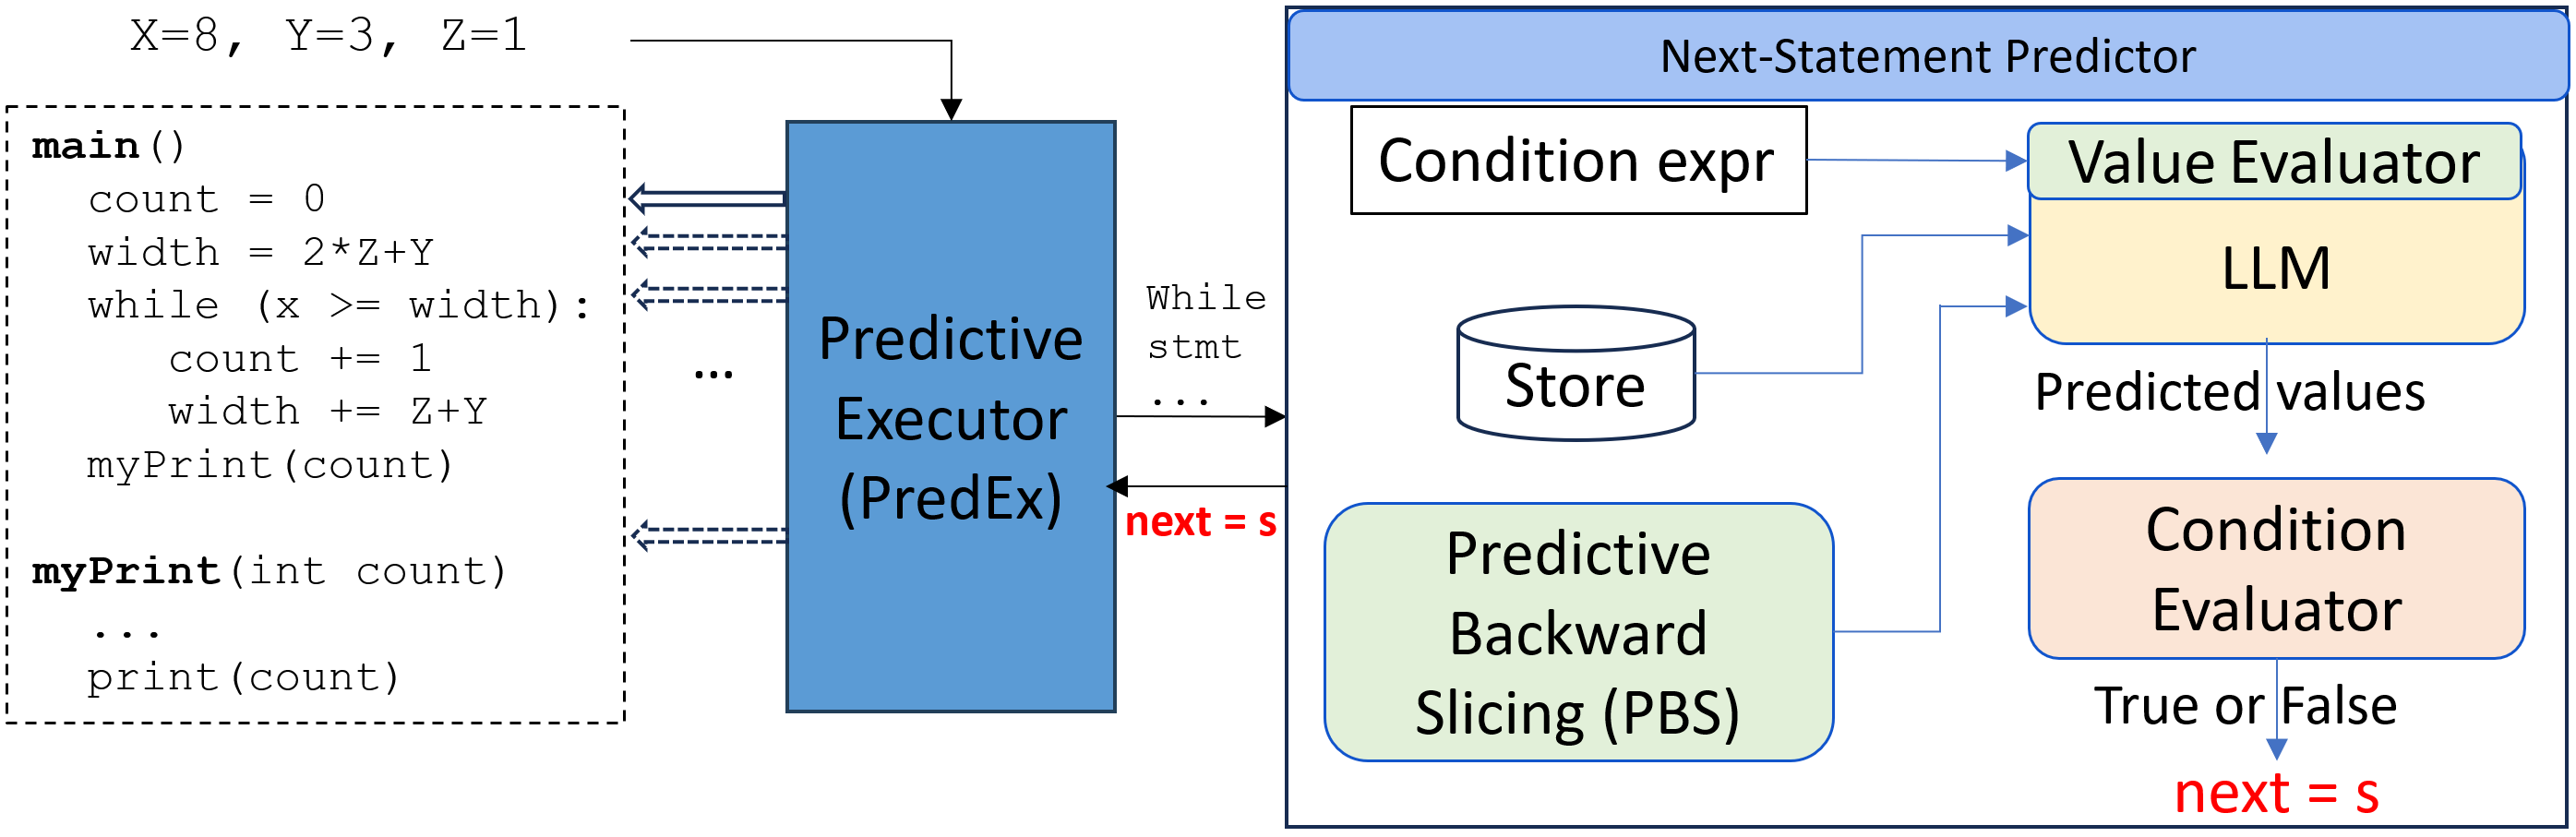
\includegraphics[width=4in]{overview-4.png}
\vspace{-22pt}
\caption{PredEx: Blended Analysis Framework for Predictive Execution}
\label{fig:overview}
\end{center}
%\end{figure*}
\end{wrapfigure}

In blended analysis, we decompose the original problem into smaller sub-tasks and allocate~each task to either PA or LLM based on their respective strengths. At the coarse-grained level, we divide the predictive execution problem into predicting the next executed statement at each step. When PA can make deterministic decisions, such as determining the next executed statement within a block, we leverage PA for that to alleviate the potential inaccuracy of the LLM. However, when PA is unable to ascertain the execution flow, particularly at branching points (e.g., \code{if}, \code{while}, \code{for}, etc.), we enlist the LLM to handle tasks critical for the decisions at those branching points. At the fine-grained level of the task of LLM-based branching decisions, we also harness PA to assist the LLM in focusing on the pertinent statements when making decisions about the branching direction. That is, we posit that by providing the LLM with support from PA and feeding it relevant statements, we can guide it in reasoning about the execution of a smaller subset of statements without executing them. Via pre-training, LLMs have learned patterns, logic, and reasoning capabilities that enable them to predict program execution for a smaller set of statements relevant to branching decisions.

%=====================================================
Specifically, the two sub-tasks at a branching point for the LLM
include {\em value evaluator} and {\em condition evaluator}. First, the value
evaluator focuses on determining the values of variables involved in
decision-making at a branching point. By using backward slicing
starting from those variables, we can help the LLM focus only on the
relevant, important statements that influence the values of the
variables. We build the backward slices and use the current predicted
statements and paths in the trace to approximate the dynamic backward
slice. Let us call it {\em predictive backward slice}. By such slices
and predicted values, we enable the LLM to recognize patterns and
dependencies in the code that affect the values of the current
variables. By training the LLM via few-shot learning on the external
API calls, we enable it to derive the output values of such calls.
Second, the condition evaluator, builds on the values obtained from
the value evaluator. Given the values of the variables at a branching
point, the condition evaluator can predict the outcome of the
condition expression. For this evaluation, one can have different
strategies. First, one can leverage the LLM as in the value
evaluator. Second, one can leverage the expression evaluator. Third,
one could build his/her own probabilistic condition evaluator to
estimate the probability of the condition being true.



%Fig.~\ref{fig:overview} shows an overview of PredEx. It accepts a
%Python program and input values. Its output is the predictive
%execution trace, i.e., the order of the statements that would be
%executed. The principle in PredEx is a {\bf blended analysis} between
%{\bf program analysis} and {\bf Large Language Model (LLM)}. The
%blended analysis is expressed in two folds. \underline{First}, when PredEx is
%certain on the execution order of the next statement $s$ based on the
%current statement, it will add $s$ into the resulting predictive
%execution trace. Only when it is not certain, e.g., at a branch of an
%\code{if} statement with an uncertain condition, PredEx requests its
%next-statement predictor (NSP) to provide the prediction of the
%potential next statement. \underline{Second}, even though we leverage LLM to
%predict the values of relevant variables and sub-expressions in the
%condition expression of a statement with a branching instruction, we use
%{\bf program analysis}, specifically the {\bf predictive backward slicing},
%to help the LLM pay attention only to the statements that might affect
%the evaluation of the condition. The backward slice for a variable
%might be long, thus, we design a strategy to optimize and shorten the
%slice by storing the predicted values of relevant variables at the
%latest prediction~point.

%With the blended analysis, we break down the task of predicting the
%execution into a smaller sub-tasks and leverage the deterministic
%nature of some sub-tasks (e.g., unconditional execution). We expect to
%help the LLM better decide the next executed statement.  In fact, in
%our empirical evaluation, PredEx improves over the state-of-the-art
%approaches, GPT-3.5~\cite{ChatGPT} and CodeExecutor~\cite{liu2023code},
%in which the source code and input are fed into the LLM to produce the
%entire execution trace.

\subsection{Predictive Execution: Illustrating Example}
\label{sec:example}

%\begin{figure}[htp]

\begin{wrapfigure}{r}{0.5\textwidth}
%\begin{figure}[t]  
\begin{center}
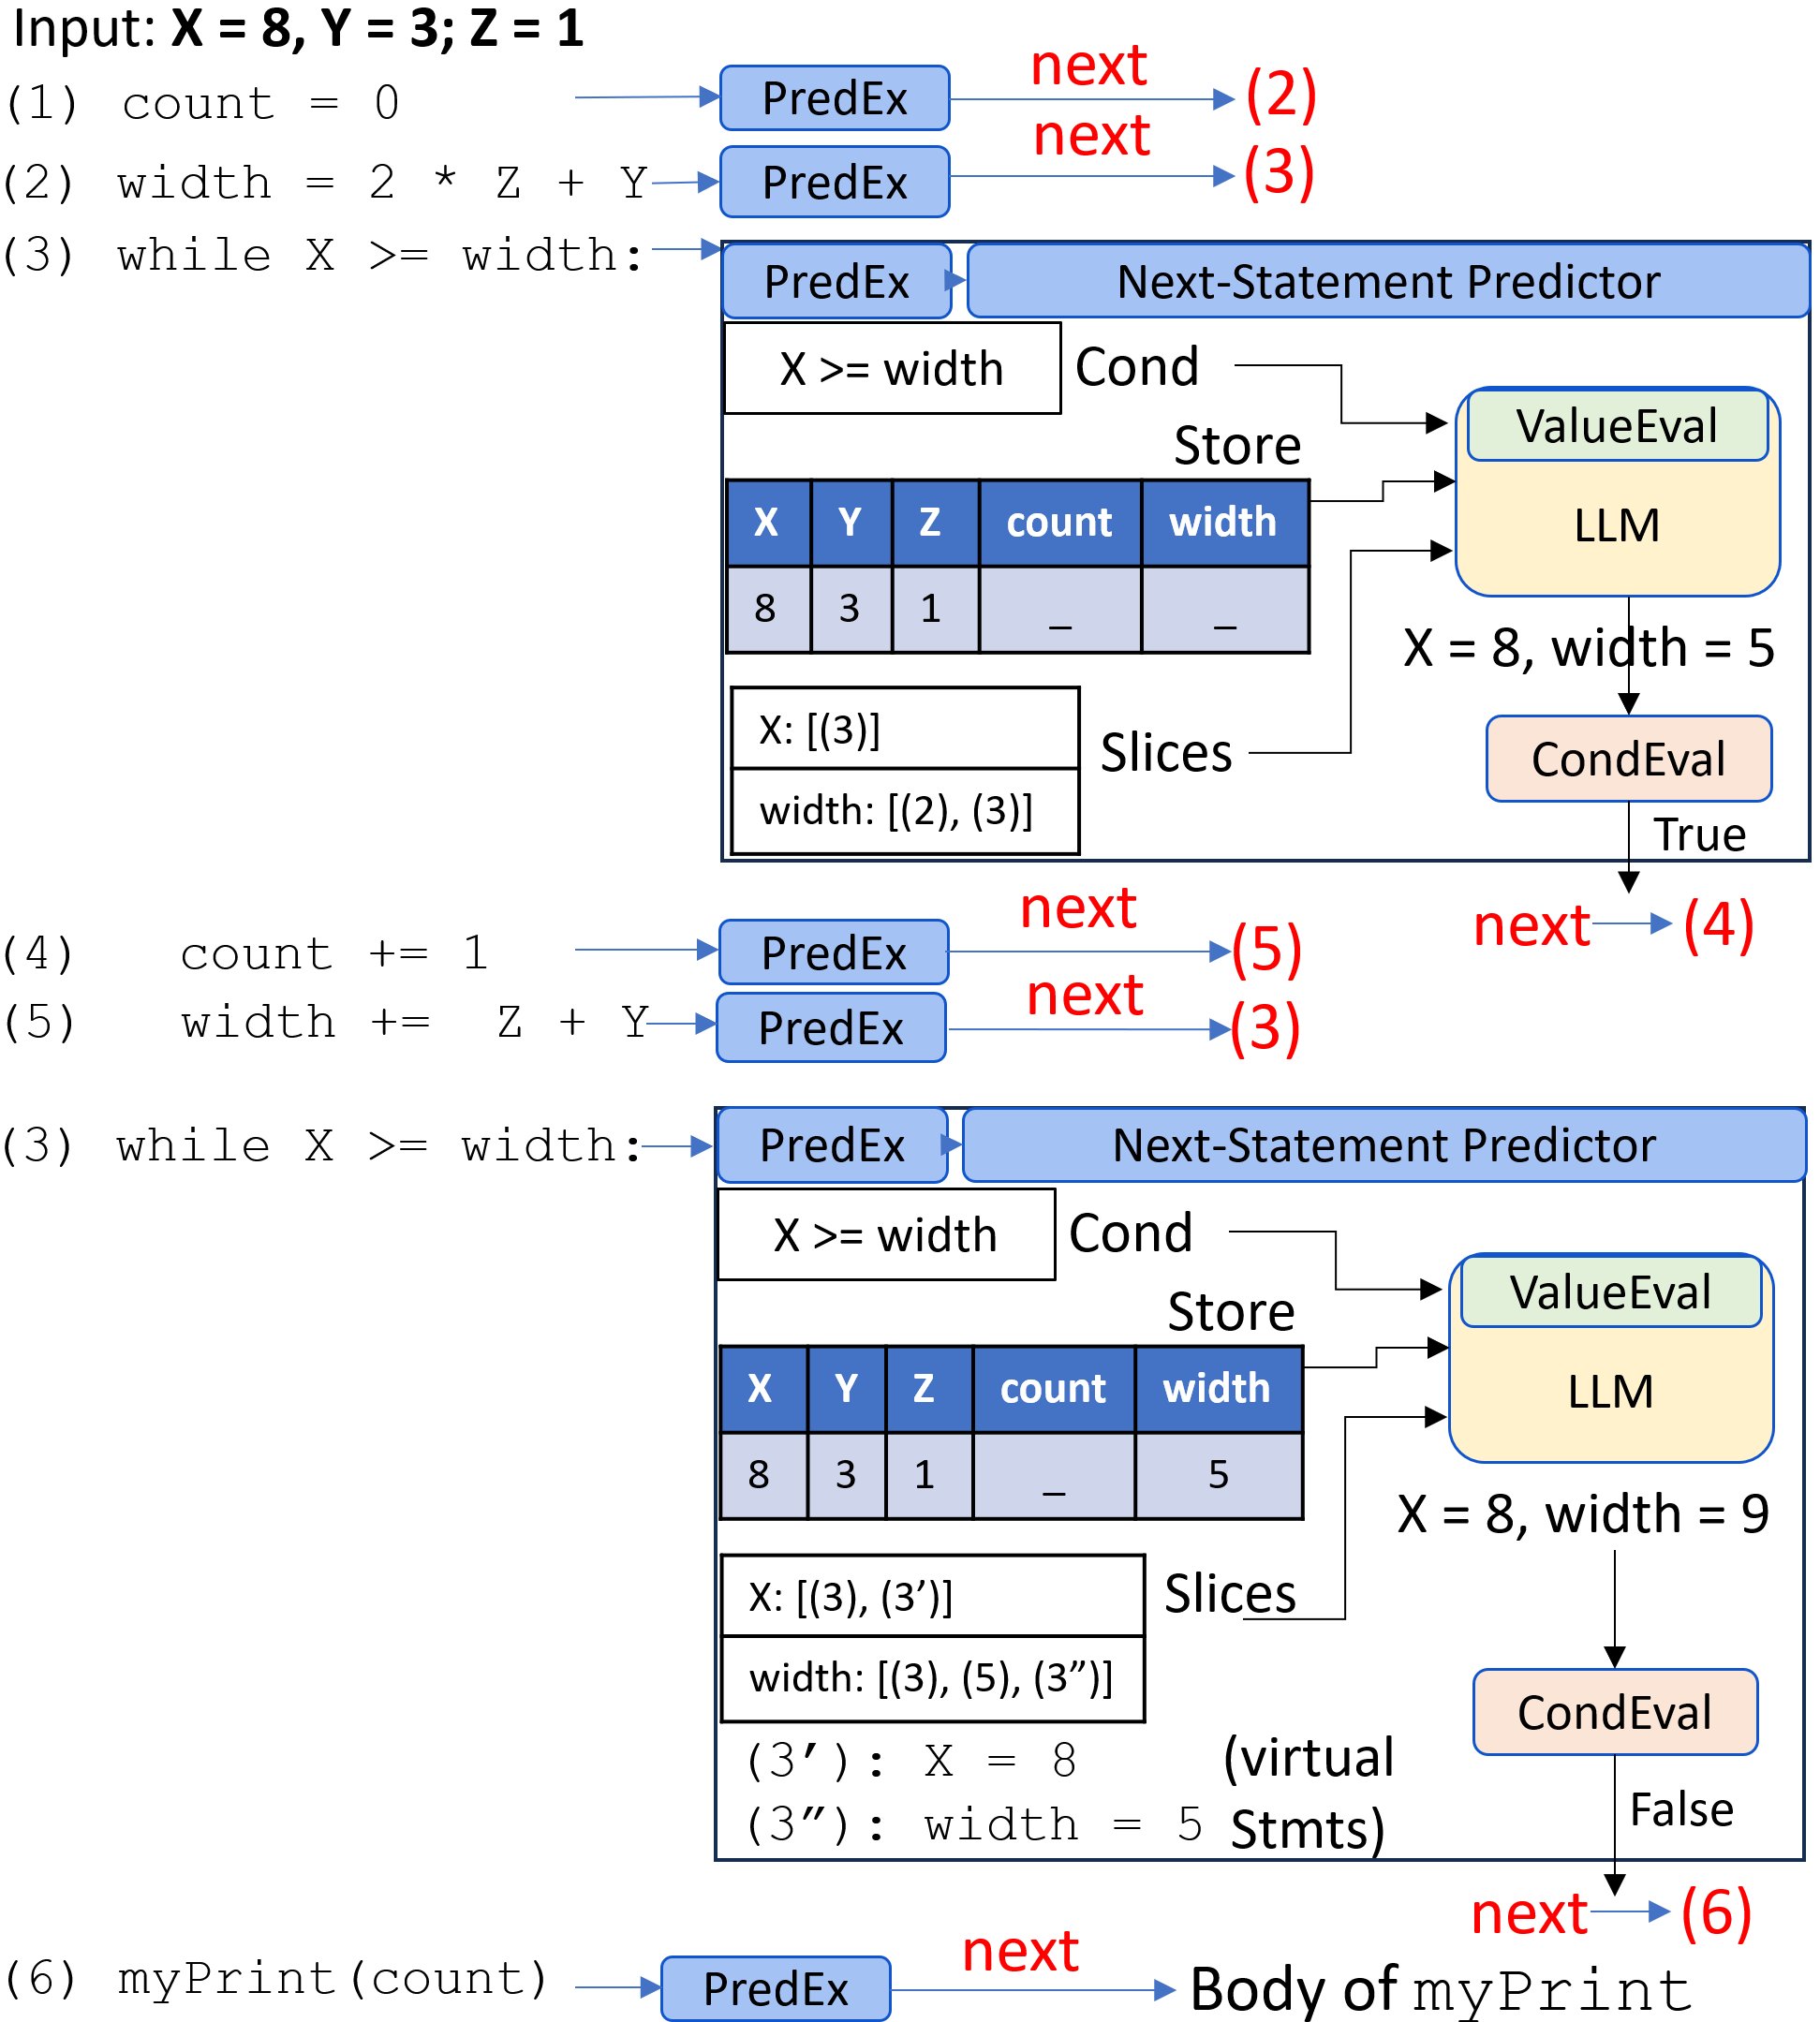
\includegraphics[width=3.2in]{example-4.png}
\vspace{-13pt}
\caption{Predictive Execution: An Illustrating Example}
\label{fig:illustration}
\end{center}
%\end{figure}
\end{wrapfigure}

Fig.~\ref{fig:illustration} illustrates how PredEx works on our
motivating example. For brevity in the figure, we use the new input
\code{X}=$8$, \code{Y}=$3$, and \code{Z}=$1$. Assume that, PredEx
starts with the assignment at line (1). Because line (1) is a simple
statement, PredEx decides the statement (2) to be the next
one. Similarly, PredEx decides the statement (3) as the one after
that.

At line 3, encountering a \code{while} statement, PredEx passes the
information on to the next-statement predictor. This LLM-based value
evaluator requires three pieces of information as
input. First, PredEx extracts the condition expression \code{X >=
  width}. Second, the current state of the value store $\theta$ includes the
initial values for the variables \code{X}=$8$, \code{Y}=$3$, and \code{Z}=$1$, and
the undefined values for \code{count} and \code{width} because those are the
values from the latest prediction point (also referred to as {\em
  check point}). If there is no prediction point yet, the latest check
point is at the very beginning. Third, PredEx computes two predictive
slices for the two variables involving in the condition
\code{X>=width}. The slice for \code{X} includes only the statement at line
(3), while the slice for \code{width} includes two statements at line (2)
and line (3).

From the three pieces of information, the LLM-based value evaluator
predicts the values of \code{X}=$8$ and \code{width}=$5$. After the store is
updated, the condition evaluator
will use it to evaluate \code{X>=width} and return $True$. To reduce
the number of requests to the LLM to update the values for all
variables, we only update the values of the variables involving in the
condition. For example, the value of the variable \code{count} is not
updated. The next prediction for the second iteration
will use the updated values in the store $\theta$. Because the
condition is predicted as $True$, the next-statement predictor will
return the statement (4) as the one.
%
Because the statement (4) is simple, PredEx decides the
statement (5) as the next one. Similarly, it moves on to
the statement (3) after that.



At the second iteration for the \code{while} statement at line 3,
PredEx also utilizes the next-statement evaluator. The condition is
the same: \code{X>=width}. However, the store $\theta$ is updated with
the latest predicted values: \code{X}=$8$, \code{Y}=$3$, \code{Z}=$1$,
\code{count}=$\_$, and \code{width}=$5$. To compute the backward
slices for \code{X} and \code{width}, PredEx performs differently
from the last time. Because in the previous prediction point, \code{X}
was evaluated to 8 and \code{width} was evaluated to 5, we create two
virtual statements: 1) statement (3'): \code{X}=$8$, and 2) statement
(3''): \code{width}=$5$ at the beginning of the loop (right after the
statement (3)). The predictive backward slice for \code{X} is computed
as containing the statement (3) and the new one (3'). Due to the new
virtual statement with the updated value of \code{width}, we only need
to include into the predictive backward slice for \code{width} the
statement (3), (5), and (3''). We do not need all the statements from
the beginning up to that point. That is, we do not include the
statement (2) into the PBS for \code{width} at this iteration.

With the condition \code{X>=width}, the store $\theta$, and the above
slices, the LLM-based value evaluator predicts the values \code{X}=$8$
and \code{width}=$9$. At this iteration, the condition evaluator
returns $False$, and the next statement is the statement (6), i.e.,
the loop ends.  For statement (6), PredEx will move on to
\code{myPrint()}.

%The statement (6) is an expression statement, which is an expression
%in the form of a function call to \code{myPrint(...)}. PredEx will
%move on to make prediction for the statements in the body of the
%\code{myPrint} function. The process continues until the end or
%\code{ERROR} occurs.

%\section{Thrust 1. Neural Structural Analysis Infrastructure}
\label{sec:thrust1}

\subsection{Planned Work on Syntactic Type Tagging and Partial AST Building}

\begin{wrapfigure}{r}{0.3\textwidth}
\begin{lstlisting}[basicstyle=\scriptsize\sffamily, stepnumber=1, numbers=left, numbersep=-6pt, framexleftmargin=0mm, framexrightmargin=0mm, language=Python, emph ={}]
    for element in item_list:
        if element > 0:
            value += 1
        else:
            selected = element
            break
\end{lstlisting}
\vspace{-0.1in}
\caption{Running example}
\label{run_ex}
\end{wrapfigure}

Let us consider the Python code snippet illustrated in Figure~\ref{run_ex} as a running example in this section. For the {\em syntactic type tagging} task (essentially a lexical classification), the goal is to tag the code tokens with their corresponding syntactic unit types like variables, fields, methods, classes, etc. For example, the code tokens in the running example would correspond to \code{FOR}, \code{LOCAL\_VARIABLE}, \code{IN}, ..., \code{=}, \code{LOCAL\_VARIABLE}, \code{BREAK}. 

Next, consider the task of building an abstract syntax tree for incomplete code. As mentioned in Section~\ref{sec:intro}, PPA~\cite{ppa08} accomplishes this task in a best-effort manner by means of a rule-based strategy that also involves eliminating tokens to achieve the desired intermediate representation. Thus, it is limited. Alternatively, we hypothesize that such a representation for partial programs can be learned from the ASTs of the whole programs in the existing code repositories. We plan to enable such a learning process by modeling the AST-building task as a {\em structured reordering} problem. First, during the training phase, we will collect pairs of source code tokens and their respective AST representations. Second, we will convert the ASTs into binary trees by: (a) merging a unary non-terminal node with its child to form a new non-terminal node; (b) adding a special {\em \#}-node to binarize the $n$-ary nodes~\cite{https://doi.org/10.48550/arxiv.2206.11719}. An example of the same is illustrated in Figure~\ref{fig:ast-bt-mapping}, where the sub-AST corresponding to lines 2--3 in the running example is binarized. Third, we will linearize the binary trees thus formed using a tree-traversal algorithm (inorder, pre-order, or post-order). Fourth, given sequence pairs of code tokens and corresponding linearized binary tree representations, we will carry out the structured reordering as a sequence-to-sequence neural machine translation (NMT) task. By design, the number of tokens on the target side in this NMT problem is the sum of the number of tokens in the program on the source side and the number of non-terminal tokens in the binarized AST.

\begin{figure}[h]
    \centering
    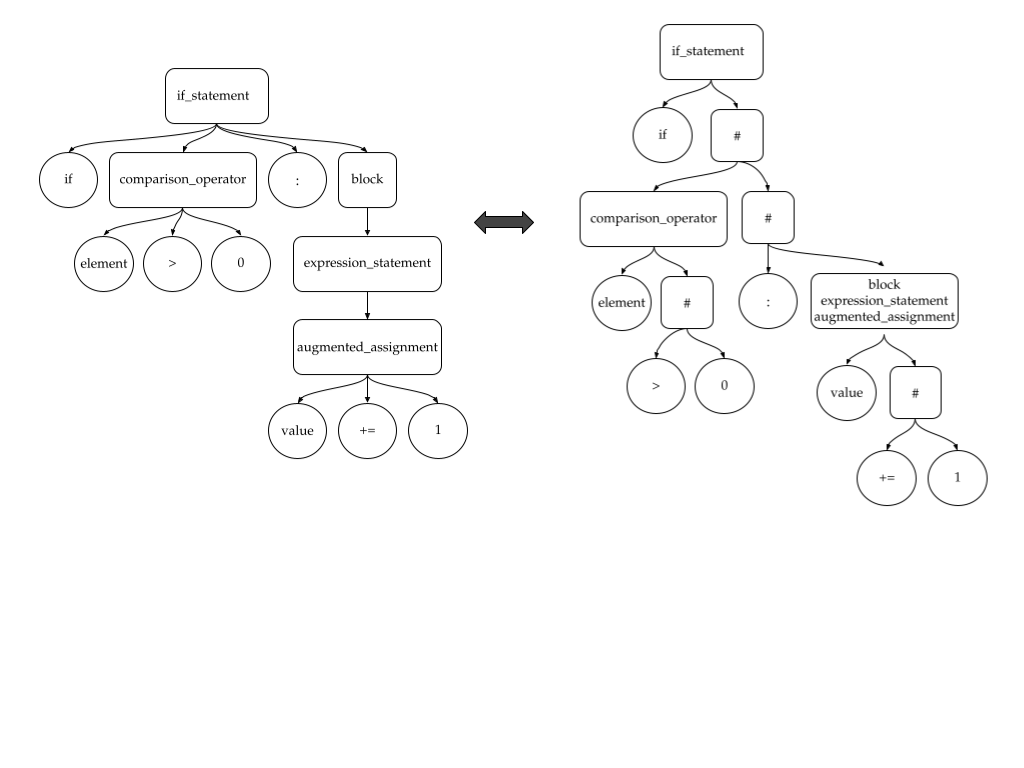
\includegraphics[width=\textwidth]{figures/ast-bt.png}
    \vspace{-130pt}
    \caption{Mapping an abstract syntax tree to its corresponding binary tree}
    \label{fig:ast-bt-mapping}
\end{figure}

For inference, one such trained NMT model can be leveraged to predict the linearized binary tree representation of the partial program under study.
The linearized binary tree representation can be used to reconstruct a unique binary tree (because of the one-to-one correspondence between them), and consequently the AST of the partial program. Moreover, the syntactic token types give information about a code token and its neighbors. Therefore, we plan to carry out both tasks, i.e., {\em syntactic-type tagging} and {\em partial AST-building} as a joint-learning process, which will help avoid error propagation from the former to the latter while benefiting each other. In addition, we will modify the decoding step in the NMT task to ensure that the ASTs thus generated for the partial programs are syntactically valid.


\section{Thurst 2. Neural Semantic Analysis Infrastructure}
\label{sec:thrust2}

\subsection{Planned Work on Type Inference for Partial Code}
\label{sec:statype}

\subsubsection{An Example of a StackOverflow Code Snippet}

\begin{wrapfigure}{l}{0.55\textwidth}
\begin{lstlisting}[basicstyle=\scriptsize\sffamily, stepnumber=1, numbers=left, numbersep=-6pt, framexleftmargin=0mm, framexrightmargin=0mm, language=Java, emph ={Event,sinkEvents,iframe,setEventListener,EventListener,StyleElement,Document,get,createStyleElement,setInnerText,resources,css,getText,getContentDocument,getHead,getBody,appendChild,ParagraphElement,createPElement,addClassName,whatever}]
    Event.sinkEvents(iframe, Event.ONLOAD);
    Event.setEventListener(iframe, new EventListener() {
        public void onBrowserEvent(Event event) {
            StyleElement style = Document.get().createStyleElement();
            style.setInnerText(resources.css().getText());
            iframe.getContentDocument().getHead().appendChild(style);

            ParagraphElement pEl = Document.get().createPElement();
            pEl.setInnerText("Hello World");
            pEl.addClassName(resources.css().getText());
            iframe.getContentDocument().getBody().appendChild(pEl);
        }
    });
\end{lstlisting}
\vspace{-0.1in}
\caption{StackOverflow post \#34595450 on GWT Widgets~\cite{soexample}}
\label{example}
\end{wrapfigure}

StackOverflow is a good resource of high quality code snippets that
show correct API usages. However, due to the discussion context and
the informal nature of the forum, code snippets rarely contain
sufficient declarations and references to fully-qualified names.

%This example illustrates three key challenges in resolving ype
%information.

Let us use a real-world example to illustrate the 
challenges in~resolving 
the fully qualified names (FQNs) 
for an SO code snippet. Figure~\ref{example} shows a
code snippet of an answer for an SO post
%\#34595450 
on Widgets in the GWT library. 

First, the snippets are not often embedded in methods or classes. In
Figure~\ref{example}, the code does not have an enclosing method or
class.

Second, they may refer to variables whose {\em declarations are not
  included}, and~their {\em identifiers are largely unqualified}. For
example, the variable \code{iframe} at lines 1, 2, 6, and 11 do not
have a declaration because the responder assumes that users would add
a declaration of type \code{IFrameElement} for \code{iframe} or add a
method call to the API \code{createIFrameElement} to get an object of
the type \code{IFrameElement}.
%
%\code{iframe} was declared earlier with the type \code{IFrameElement}
%a declaration of the type \code{IFrameElement} for \code{} 
%or an access to such an object by a prior call to
%\code{createIFrameElement}. 
%

Third, {\em the external references in code snippets are also often
  undeclared}. Specifically, code snippets frequently refer to
external types without specifying their FQNs since the
responder assumes that those FQNs could be implicitly understood in
the context of~the post.
%Tien
%
%assumes that users would add the required imported libraries when
%using the snippet in their programs in an IDE.
%
%
For example, the types \code{Event}, \code{EventListener},
\code{StyleElement}, \code{Document}, and \code{ParagraphElement} are
referenced by simple names only. Fourth, {\em name ambiguity occurs in
  the references to external libraries}. For example, the type
\code{EventListener} at line 2 is a common unqualified type name. In
this snippet, it refers to
\code{com.google.gwt.user.client.\-Event\-Listener}. However, it is
ambiguous with \code{java.util.EventListener} in JDK. Similarly, the
simple type name \code{Document} at line 4 is also popular
(\code{com.google.gwt.dom.client.Document},
\code{org.eclipse.jface.text.Document}, \code{org.w3c.dom.Document},
etc).
%Thus, if the code snippet is placed inside a class within an IDE, it
%will not be compiled due to missing \code{import} statements for
%needed packages.
%In fact, the phenomenon of 
In fact, external reference ambiguity is
popular~\cite{dagenais-icse12}.
%has been reported before.
%by Dagenais and Robillard~\cite{dagenais-icse12}: 89\% of method names
%in their study are ambiguous and on average, a method name has 13
%candidate FQNs.
%
%Subramanian {\em et al.}~\cite{liveapi14} reported that 
For example, the simple names \code{getId} and \code{Log} occur 27,434
and 284 times respectively in various Java libraries~\cite{liveapi14}.


%In a later version, it uses a dictionary of all the APIs of the
%libraries of interest. This is tedious to build a dictionary.


To address those ambiguities,
%in resolving the FQNs, for the elements in a code snippet,
existing approaches rely on rules and heuristics mainly from
program analysis. 
%
%ACE~\cite{rigby-icse13} focuses on resolving types for API names
%within texts via text analysis of the enclosing SO posts, thus, is
%inapplicable for this example.
%
RecoDoc~\cite{dagenais-icse12} uses heuristics in the partial program analysis tool,
PPA~\cite{dagenais-oopsla08}, 
%to apply heuristics on syntactic constructs to recover the declared
%types of certain expressions (\eg assignments). Unfortunately, 
however, in many cases, the heuristics help recover only partially
qualified names, due to much missing information. For example, at line
6, Figure~\ref{example}, the types of the receiver \code{iframe} and
method call \code{getContentDocument}, are not known. In contrast,
Baker~\cite{liveapi14} uses a dictionary of all the API names of
interest. Each API name has multiple candidates of FQNs. Baker
iteratively cuts off the candidates by overlapping the candidate lists
of API names in the same scopes in the code snippet. However, scoping
rule or other rules/heuristics are not always effective in incomplete
code snippets. In this example, lines 4--6 in Figure~\ref{example}
have only one scope with the popular API names having many potential
FQNs (\code{Document}, \code{getText}, \code{appendChild}). Moreover,
building and updating a dictionary of the APIs require
much~effort~\cite{dagenais-fse10}.


%{\em program analysis}, {\em text analysis}, or {\em deductive
%  analysis}, and/or the use of {\em an oracle of APIs of
%  interest}. 
%
%Specifically, partial program analysis (PPA)
%technique~\cite{dagenais-oopsla08} performs partial parsing and type
%resolution with several heuristics. PPA disambiguates the names by
%applying a set of heuristics on the syntactic constructs to recover
%the declared types of certain expressions in an incomplete code
%snippet. Unfortunately, in many cases, the heuristics help recover
%only partially qualified names, due to much missing information. For
%example, at line 6, the types of the receiver, method call, and
%arguments are not known.
%
%RecoDoc~\cite{dagenais-icse12} suffers the same issues since it uses
%PPA to link an API and documentation.
%
%ACE~\cite{rigby-icse13} focuses on resolving types for API names
%within texts via text analysis of the enclosing SO posts, thus, is
%inapplicable for this example. 
%Baker~\cite{liveapi14} uses a dictionary of all the API names of
%interest. Each API name has multiple candidates of FQNs.  Baker
%iteratively cuts off the candidates by overlapping the candidate lists
%of API names in the same scopes in the code snippet. However, scope
%rules are not always effective in incomplete code with few scopes or
%in popular names with many potential FQNs, \eg \code{Document},
%\code{getText}, \code{appendChild} on lines 4--6. Moreover, building
%and updating an oracle of the APIs require
%much~effort~\cite{dagenais-fse10}.

%=========================================================================
%To address those ambiguities in resolving the FQNs for the elements in
%a code snippet, existing approaches rely on {\em program analysis},
%{\em text analysis}, or {\em deductive analysis}, and/or the use of
%{\em an oracle of APIs of interest}.
%
%Specifically, partial program analysis (PPA)
%technique~\cite{dagenais-oopsla08} performs partial parsing and type
%resolution with several heuristics. PPA disambiguates the names by
%applying a set of heuristics on the syntactic constructs to recover
%the declared types of certain expressions in an incomplete code
%snippet. Unfortunately, in many cases, the heuristics help recover
%only partially qualified names, due to much missing information. For
%example, at line 1, the types of the receiver, method call, and
%arguments are not known. RecoDoc~\cite{dagenais-icse12} suffers the
%same issues since it uses PPA to link an API and documentation.
%ACE~\cite{rigby-icse13} focuses on resolving types for API names
%within texts via text analysis of the enclosing SO posts, thus, is
%inapplicable for this example. Baker~\cite{liveapi14} uses a
%dictionary of all the API names of interest. Each API name has
%multiple candidates of FQNs.  Baker iteratively cuts off the
%candidates by overlapping the candidate lists of API names in the same
%scopes in the code snippet. However, scope rules are not always
%effective in incomplete code with few scopes or in popular names with
%many potential FQNs, \eg \code{Document}, \code{getText},
%\code{appendChild} on lines 4--6. Moreover, building and updating an
%oracle of the APIs require much~effort~\cite{dagenais-fse10}.
%=======================================================================

%--------------------------------------------------------------
%To address those ambiguities in resolving the FQNs for the program
%elements in a code snippet, existing approaches rely on {\em program
%  analysis}, {\em text analysis}, and/or the use of {\em an oracle of
%  APIs of interest}. Specifically, partial program analysis (PPA)
%technique~\cite{dagenais-oopsla08} performs partial parsing and type
%resolution with several heuristics. PPA disambiguates the names by
%applying a set of heuristics on~the syntactic constructs to recover
%the declared types of certain expressions in an incomplete code
%snippet. Unfortunately, in many cases,~the heuristics help recover
%only partially qualified names, due to much missing information.  For
%example, at line 1, the types of the receiver, method call, and
%arguments are not known. RecoDoc~\cite{dagenais-icse12} suffers the
%same issues since it uses PPA to link an API and documentation. With
%context analysis, ACE~\cite{rigby-icse13} analyzes the API names by
%considering the {\em textual contexts} surrounding them in SO
%posts. However, it might not be always effective since the surrounding
%texts might not be sufficient and code snippets were not analyzed.
%Baker~\cite{liveapi14} uses a dictionary of all the API names in the
%libraries of interest. Each API name has multiple candidates of FQNs.
%Baker iteratively cuts off the candidates by overlapping the candidate
%lists of multiple names in the same scopes in the code
%snippet. However, scope rules are not always effective in incomplete
%code or in popular names with many potential FQNs, \eg
%\code{Document}, \code{getText}, \code{appendChild} on lines 4--6.
%Thus, after its process, the resulting API names from Baker still have
%multiple potential FQNs. Moreover, building and updating an oracle of
%the APIs require much~effort~\cite{dagenais-fse10}.
%-----------------------------------------------------------------

%is also time-consuming.

%
% many API elements have
% more than one potential fully qualified type names

%problem with oracle
%overlapping

%\vspace{-0.14in}
\subsubsection{Key Ideas in {\tool}}

%type references, method calls, and field references.

%resolve the simple names

As part of {\tool}, we will develop a technique to identify the FQNs for
the simple names of {\em variables, API classes, method calls, and
  field accesses} in a code snippet in online forums.
%
In our solution, we leverage two kinds of context in deriving FQNs for
API elements. 

The first one is the {\em type context} of API elements in a
large code corpus. 
%FINAL
%Hindle {\em et al.}~\cite{natural} has shown that software exhibits
%its naturalness: source code has a higher degree of regularity than
%English texts. We expect the same principle of naturalness of software
%to occur for the API elements in the API code usages. 
That is, in the API usages, the API elements including API classes,
method calls, and field accesses of software libraries do not occur
randomly. They appear regularly with certain other API elements due to
the intent of the libraries' designers to provide certain
functionality in API usages. For example, to manipulate style
information for a frame in GWT, at lines 4--6 in Figure~\ref{example},
a \code{StyleElement} in GWT could be created via a call to
\code{createStyleElement} of a \code{Document} object. Then, the style
is assigned with a name via \code{StyleElement.setInnerText} and
associated with an \code{IFrameElement} object. Those API elements of
those types repeatedly occur together because such tasks are provided
by the GWT library and intended via such API usages. Thus, if {\tool}
observes the API usages involving those API elements in a large corpus
of programs using GWT, it can use the context of the given code
snippet to derive the most likely FQNs for the APIs in the
snippet. For example, the context of the API names
\code{StyleElement}, \code{Document}, and \code{createStyleElement}
could give {\tool} a hint on the FQNs of the undeclared variable
\code{iframe}, the method calls \code{getContentDocument},
\code{appendChild}, and vice versa.
To learn the context, we rely on the basis of regularity with a large
corpus: the API elements regularly going together in API
usages have higher impact in deciding the FQNs than the less
regular~ones.

%ones that
%are project-specific and less likely to appear frequently~together.

%To learn the context, we rely on the basis of regularity with a large
%corpus containing the APIs of interest. That is, the API elements that
%regularly go together in API usages will have higher impact in
%deciding the FQNs than the ones that are project-specific and less
%likely to appear frequently~together. 

%
%For example, with a large corpus of programs using GWT, a model could
%learn that \code{com.google.gwt.user.client.Event.setEventListener}
%often goes with \code{com.google.gwt.user.client.Event.EventListener},
%and \code{com.google.\-gwt.user.client.Event.sinkEvents}.

The second context is called {\em resolution context} on how the types
of API names surrounding an API name have been resolved. The
undeclared/ambiguous references are expected to be disambiguated with
{\em the most likely FQNs with regard to the FQNs of the surrounding
  names}.
%
For example, at lines 3--4, when resolving \code{Event},
\code{StyleElement}, and \code{Document}, we could use an effective
search strategy to maintain the sequences of FQNs with the highest
probabilities. For \code{Event}, we have multiple candidates. However,
if we chose \code{com.google.gwt.user.client.Event} for \code{Event},
then based on their regularity, we could maintain the option
\code{com.google.gwt.dom.client.Document} for \code{Document}, with a
higher score than \code{org.w3c.dom.Document}. Finally, the sequence
with the highest score will be reported as the~result.

%Then, we use it to decide the type for the next API.

%with a large corpus of programs using GWT, a model could
%learn that \code{com.google.gwt.user.client.Event.setEventListener}
%often goes with \code{com.google.gwt.user.client.Event.EventListener},
%and \code{com.google.\-gwt.user.client.Event.sinkEvents}.



% ---- old ---
%In this work, to realize that philosophy, we use a data-driven
%approach with the two following key ideas:

%1) In the context of API usages, certain API elements need to be used
%together because they have to follow the API specifications. For
%example, with a large corpus of programs using GWT, a model could
%learn that \code{com.google.gwt.user.client.Event.setEventListener}
%often goes with \code{com.google.gwt.user.client.Event.EventListener},
%and \code{com.google.\-gwt.user.client.Event.sinkEvents}.
%To learn the contexts, we rely on the {\bf basis of regularity} with a
%large corpus containing the APIs of interest. That is, the API
%elements that regularly go together in API usages will have higher
%impact in deciding the FQNs than the ones that are project-specific
%and less likely to appear frequently~together.

%2) To narrow the candidate FQN list for an API name, we could use the
%{\bf context of its surrounding API names}. The undeclared/ambiguous
%references are expected to be disambiguated with the most likely FQNs
%with regard to the FQNs for surrounding names.
%------------------------------------------------------------

%
%\code{com.google.gwt.user.client.Event.sinkEvents} receives two
%arguments of the types \code{com.google.gwt.dom.client.Element} and
%\code{int}, and it often goes with
%\code{com.google.gwt.user.client.Event.setEventListener}, etc.
%
%For example, at line 1 of Figure~\ref{example}, even though we do not
%have the declaration of \code{iframe}, however, with the large corpus
%of open-source projects, the model could learn that the method
%\code{com.google.gwt.user.client.Event.sinkEvents} receives two
%arguments of the type \code{com.google.gwt.dom.client.Element} and
%\code{int}, and it often goes with
%\code{com.google.gwt.user.client.Event.setEventListener}.


%Tien
%\input{rules.tex}
%\input{smt-motiv}



%2) {\em Second}, because the translation takes into account {\bf the
%  context consisting of surrounding API elements/names}, the
%undeclared/ambiguous references will be disambiguated with the most
%likely FQNs with regard to the FQNs of their surrounding names.

%3) ambiguity: Third, not all the changes in the current context are useful in
%recommendation because they can be project-specific and considered
%as noise in the change patterns. Recent work [41] confirms
%that not all code changes are repetitive. To address this, we rely on
%the basis of consensus: given a large number of changes in many
%projects, the project-specific changes are less likely to appear frequently
%than the changes belonging to a higher-level intent pattern.
%-==> undeclared types


\subsection{Preliminary Work on Neural Program Dependence Analysis}
\label{sec:deeppda}

In the neural network-based dependency
parsing~\cite{chen-manning-2014-fast} in NLP, by projecting the words
into an embedding space, researchers successfully learn the semantic
relationships that model the dependencies between them. We can follow
suit to learn the control-flow and program dependencies between the
statements in programs as well. Moreover, given that the quality of
the statement embeddings determines the accurate prediction of the
program dependence relations, enhancing them by incorporating context
from both within and across the statements is crucial. Intra-statement
contextualization can help relay the local information within
individual statements globally. For example, such information can help
distinguishably identify the declaration and reference of the same
variable across  program statements. In contrast,
inter-statement contextualization helps learn the dependencies between
the statements in the context of the surrounding statements. Finally,
we aim to model the CFG/PDG construction as a pairwise dependence
decoding task, wherein the combination of all the predicted edges in
the statement pairs can be formalized as directed graphs, e.g., CFG/PDG.

\begin{figure*}[t]
\begin{center}
    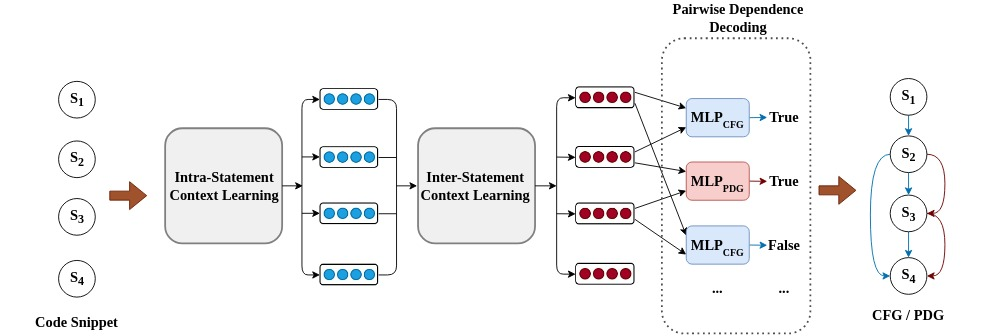
\includegraphics[width=0.9\textwidth]{model-abstract.jpg}
    \caption{Preliminary Design for \tool Model Infrastructure for Dependency Analysis for Partial Code}
    \label{fig:model}
    \vspace{-26pt}
\end{center}
\end{figure*}

%In Figure~\ref{fig:model}, we present a preliminary design of the
%general architecture of \tool model.

%Given that attention is the driver behind the now ubiquitous
%Transformers’~\cite{Vaswani-2017} success in efficiently learning
%representations for different entities in different contexts, we plan
%to make it the foundation of the context learning components in our
%model as well. Each is intended to learn different aspects of
%contextualization.

%\begin{figure*}
%    \centering
%  \subfloat[Intra-Statement Context Learning\label{fig:input_repr_a}]{%
%       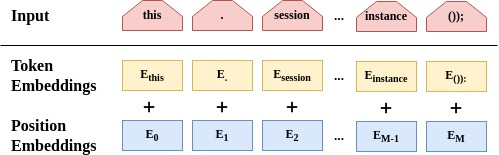
\includegraphics[width=0.45\linewidth]{figures/input_repr_tok.jpg}}
%  \hspace{0.25cm}
%  \subfloat[Inter-Statement Context Learning\label{fig:input_repr_b}]{%
%        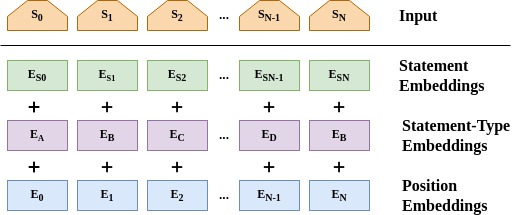
\includegraphics[width=0.45\linewidth]{figures/input_repr_stmt.jpg}}
%    \hfill
%  \caption{Input representations: (a) tokens in a statement are the sums of token embeddings, and (token) position embeddings; (b) statements in a snippet are the sums of statement embeddings, statement-type embeddings, and (statement) position~embeddings.}
%  \label{fig:input_repr}
%\end{figure*}


%\subsection{\bf Model Architecture}
%\label{sec:ppda_arch}

%As explained in Section~\ref{sec:overview}, better contextualization
%is the main idea behind \tool's design. Given that attention is the
%component in the ubiquitous Transformers'~\cite{Vaswani-2017} success
%in efficiently learning representations for different entities in
%different contexts, we chose to make it the foundation of our
%model. In brief, we realize \tool via a hierarchical, self-attention
%network (SAN)-based model architecture, where each sub-network is
%intended to capture different aspects of contextualization. Its
%details are as follows:

\vspace{2pt}
\subsubsection{{\bf Intra-Statement Context Learning (IntraS-CL)}}
\label{sec:ppda_arch_intra}
The syntactic and semantic knowledge of the code tokens within a
single statement must be made available globally to other statements
in a program to learn the inter-statement program dependencies
effectively. We enable this via a \textit{1-Layer} (i.e., $N_X$$=$$1$)
Self Attention Network (1L-SAN). The self-attention layer in an 1L-SAN
inputs $x_1, x_2, ..., x_n \in \mathbb{R}^d$, performs self-attention
once by projecting the inputs from all attention heads $\in
\mathbb{R}^{d_h}$ into the head dimension space $d_h$ via linear
transformations, and generate outputs $y_1, y_2, ..., y_n \in
\mathbb{R}^d$ which are linear combinations of the concatenated
attention head values. We use one attention head
(i.e., $h$$=$$1$) for the self-attention layer in 1L-SAN, and the size
of the input representations, i.e., $d$ is set to 512. Our experiments
revealed only a marginal performance gain by expanding the 1L-SAN to a
2L-SAN, which also came with high computational
overhead. Besides, increasing the number of attention heads did not
help either performance or interpretability. A more detailed analysis
on hyperparameters and subsequent
trade-offs is left to future~work.

\vspace{1pt} \underline{Input Representations}. For a program
comprising $N$ statements $s_1, s_2, ..., s_N$, \tool takes as input a
concatenation of $N$ sequences of $M$ tokens each, $\langle
t_1^{(1)}$, $t_2^{(1)}$.., $t_M^{(1)} \rangle$, ..., $\langle
t_1^{(N)}$, $t_2^{(N)}$.., $t_M^{(N)} \rangle$. Next, each token
sequence $\langle t_1^{(i)}$, $t_2^{(i)}$.., $t_M^{(i)} \rangle$ is
input to the 1L-SAN for intra-statement contextualization. Previous
works~\cite{radford2019language, liu2019roberta} have demonstrated
the~advantages of a byte-level Byte-Pair Encoding (BPE)-scheme for
tokenization. We follow suit to train a byte-level BPE tokenizer for
converting a given statement into a sequence of tokens. Here, $M$ is
the maximum number of tokens allowed in a statement.  For statements
with token sequences having ${<}M$ tokens, a special \textit{[PAD]}
token is appended. In contrast, token sequences having ${>}M$ tokens
are truncated to $M$ tokens.

%\vspace{1pt} \underline{Token Embeddings}. For all the words in the
%vocabulary $V$, we leverage a learnable embedding to learn and store
%their representations (i.e., $\mathbb{R}^{|V| \times d}$). Using this
%as a lookup table, token embeddings are retrieved for all the tokens
%generated by the tokenizer for a given statement.

%\vspace{1pt} \underline{Token Position Embeddings}. Attention
%mechanism in the self-attention layer is invariant to position
%information. However, this knowledge is key to understanding the
%sequential nature of code tokens in a statement. We enable this via
%learnable position encoding scheme, where a vector $\in \mathbb{R}^d$
%unique to each position is learned during the training process.

%\vspace{1pt} \underline{Statement (Output) Representations}. Input
%representations to the 1L-SAN corresponding to the tokens in a given
%statement are taken as the sums of the \textit{token embeddings}, and
%their \textit{position embeddings} (as in
%Fig.~\ref{fig:input_repr_a}). The 1L-SAN yields intra-statement
%contextualized token representations as its output, which are then
%averaged to retrieve the statement representation. Note that the token
%representations corresponding to the \textit{[PAD]} tokens are not
%considered for averaging. Such statement representations $u_i$ ($\in
%\mathbb{R}^d$) for all the statements $s_i \in s_1 ... s_N$ are then
%passed on for inter-statement contextualization.

\vspace{2pt}
\subsubsection{\bf Inter-Statement Context Learning (InterS-CL)}
The knowledge of surrounding statements in the context of a given
statement helps \tool model the dependencies between them better. We
enable this via a multi-layer bidirectional Transformer encoder based
on the work by Vaswani {\em et
  al.}~\cite{Vaswani-2017}. Owing to its common usage, we will omit
exhaustive background details on Transformers' model architecture and
will refer the readers to ~\cite{Vaswani-2017}. As shown in
Fig.~\ref{fig:model}, we denote the number of layers in the
Transformer encoder by $N_Y$, which we set to 6. We employ 4 attention
heads, i.e., $h$$=$$4$ to increase parallelization (since
$d_h$$=$$\frac{d}{h}$, i.e., $d_h$$=$$128$) and learn different
aspects of the syntactic and semantic structure in the statements,
while still being interpretable. We also set the feed-forward module
size to be 4 times that of the size of the input representations $d$,
i.e., 2048. Overall, Transformer in InterS-CL phase inputs
local context-aware statement representations $u_i \in \mathbb{R}^d$
for all statements $s_i$ in a given program, and outputs statement
representations $v_i \in \mathbb{R}^d$ that are both local and global
context-aware.

\vspace{1pt} \underline{Statement Input Representations}. For all the
statements $s_i$, statement embeddings (i.e., $u_i \in
\mathbb{R}^d$) are obtained from the 1L-SAN in the IntraS-CL phase.
$N$ is the maximum number of statements in a method in the dataset. If
a given program has less than $N$ statements,
zero vectors ($\in \mathbb{R}^d$) are padded to the inputs.

%\vspace{1pt} \underline{Statement Position Embeddings}. To make our
%model under\-stand the sequential nature of statements in a program,
%as~in Section~\ref{sec:ppda_arch_intra}, we leverage a learnable
%position encoding~sch\-eme to learn unique vectors ($\in
%\mathbb{R}^d$) for all statement~positions.

%\vspace{1pt} \underline{Statement Types}. Most neural network-based
%dependency parsers leverage parts-of-speech (POS) tags for the words
%in a sentence for better dependency learning. Thus inspired, we chose
%to associate with each statement a label indicating the
%\textit{statement type}, which is essentially the type of the AST node
%rooted at the sub-AST for the statement. We extract labels such as
%\code{METHOD}, \code{CONTROL\_STRUCTURE}, \code{BLOCK}, etc., which
%helps augment the statement with such syntactic information. We learn
%unique vectors ($\in \mathbb{R}^d$) for each of the statement types.

%\vspace{1pt} \underline{Statement (Output) Representations}. As shown
%in Fig.~\ref{fig:input_repr_b}, the input representations for the
%statements in a program are taken as the sums of the \textit{statement
%  embeddings}, \textit{statement-type embeddings}, and the
%\textit{statement position embeddings}. These are then passed on to
%the Transformer encoder, to retrieve contextualized statement representations $v_i
%\in \mathbb{R}^d$ for all the statements $s_i \in s_1 ... s_N$, that model
%the syntactic and semantic knowledge from both within and across the
%statements. After this, we obtain the contextualized statement representations.

\vspace{1pt}
\subsubsection{\bf Pairwise Dependence Decoding}
%Pairs of latent feature vectors $\langle v_i, v_j \rangle$ (1$\leq i, j\leq$ N) are taken from the sequence of intra and inter-statement contextualized statement representations corresponding to all statements in a program, to detect the presence of CFG/PDG edges between them. A combination of all such CFG/PDG edges extracted via the arc-factored approach is realized as the CFG/PDG for the given program. We leverage 2-layered multi-layer perceptron networks (one each for detecting CFG and PDG edges, i.e., MLP\textsubscript{CFG} and MLP\textsubscript{PDG} respectively) for the pairwise dependence decoding phase, which are scored as follows:

From the sequence of contextualized statement representations $v_i \in
\mathbb{R}^d$ corresponding to all the statements in a program passed
on by the Transformer encoder in the InterS-CL phase, pairs such
as $\langle v_i, v_j \rangle$ (1$\leq i, j\leq$ N) are taken to detect
the presence of CFG/PDG edges between two statements $s_i$ and
$s_j$. We leverage 2-layered multi-layer perceptron networks (each
for detecting the CFG and PDG edges, i.e., MLP\textsubscript{CFG} and
MLP\textsubscript{PDG}, respectively) in the pairwise dependence
decoding phase, which are scored as follows:
\begin{equation}
\centering
    score\textsubscript{rel}(i, j) = MLP\textsubscript{rel}(v_i \circ v_j \circ (v_i * v_j) \circ |v_i - v_j|)
\end{equation}
where $\circ$, $*$ and $|.|$ correspond to concatenation, element-wise
product, and absolute element-wise difference operations respectively;
and \textit{rel} represents either the control-flow or program
dependence relations. Attaining a $score\textsubscript{rel}(i, j) >
0.5$ represents the detection of the corresponding CFG/PDG edge from
statement $s_i$ to statement $s_j$. The combination of all the CFG/PDG
edges extracted via such an arc-factored approach is realized as the
CFG/PDG for the given program.

\subsubsection{\bf Training Process}

Training \tool requires the knowledge of ground-truth CFG and PDG edges between statements in a program. Thus, it can only be trained on complete programs (at a minimum, which are at a method-level granularity) so as to be able to leverage program analysis tools to extract them. The CFG and PDG edge information can then be utilized to compute the training objective loss (i.e., $\mathcal{L}$) for our model as follows: $\mathcal{L} = \mathcal{L}\textsubscript{CFG} + \mathcal{L}\textsubscript{PDG}$
%\begin{equation}
%    \centering
%    $$\mathcal{L} = \mathcal{L}\textsubscript{CFG} + \mathcal{L}\textsubscript{PDG}$$
%\end{equation}
where $\mathcal{L}\textsubscript{CFG}$ is the loss for CFG edge-decoding, and $\mathcal{L}\textsubscript{PDG}$ is the loss for PDG edge-decoding. Moreover, $\mathcal{L}\textsubscript{CFG}$ and $\mathcal{L}\textsubscript{PDG}$ are computed as the sums of all binary-cross entropy (BCE) losses corresponding to the CFG and PDG edge predictions between different statements in a program. Note that the inter-statement losses corresponding to the edges from/to the zero-padded statements do not contribute to either $\mathcal{L}\textsubscript{CFG}$ or $\mathcal{L}\textsubscript{PDG}$. The model parameters which are learned to minimize $\mathcal{L}$ include learnable embeddings (token, token position, statement type, and statement position), attention, Tr-FFNN (i.e., feed-forward neural network in Transformer encoder), MLP\textsubscript{CFG}, and MLP\textsubscript{PDG}.

%Overall, \tool has about 39M parameters.

\subsubsection{\bf Inference for Dependency Discovery}
\label{sec:inference}
Despite being trained on only complete code, one can leverage \tool to extract the control-flow and program dependence edges for both complete and partial code.% The following, however, are the important points of consideration:
%\textit{Statement Types}: To extract the syntactic information encoded
%in \textit{statement types}, one would need the program's AST. In
%Java, for example, this can be retrieved even if the code is
%incomplete using tools such as PPA~\cite{dagenais-2008}. However, this
%is not possible for all programming languages. In such cases, \tool
%can be trained without statement types, i.e., by computing the input
%representation for statements in a program as just the sums of the
%statement and their position embeddings. In
%Section~\ref{sec:ablation}, we demonstrate the practicality of such an
%alternative.
%\textit{ If programs with ${\leq}N$ statements}: For both complete and
%partial programs, the number of statements in which is less than the
%\textit{maximum statements} allowed in the model is
%straightforward. In such cases, \tool predicts the CFG/PDG edges from
%one statement to another by contextualizing over all the other
%statements in the program.
If a program has ${>}N$ statements, for (both complete and partial)
programs having number of statements greater than that allowed in the
trained \tool model, we have the following strategies in {\tool}: (a)
train a model with a higher value of $N$, (b) chunk the program into
$N$-statement code fragments, predict CFG/PDG edges for each of the
code fragments independently, and finally, combine the CFG/PDG
predictions for all the fragments. For example, if a trained model
allows a maximum of 16 statements, to predict for a program with 46
statements, one can break it down into code fragments with 16, 16, and
14 statements, respectively.

%A potential downside to strategy (b), however, is that a statement in
%a fragment will be contextualized only over the other statements in
%that fragment, and the control-flow and program dependencies across
%fragments will not be captured. Increasing $N$ could address this
%issue, albeit with more computational overhead.

%\end{itemize}



\section{Thrust 3. Neural Symbolic Execution Infrastructure}
\label{sec:thrust3}


\section{Thrust 4. Applications of Neural Partial Program Analysis}

\section{On-going Work on ML-based Vulnerability Detection for Code Snippets}
\label{sec:vd}


%\section{Method-Level Vulnerability Detection}
%\label{mlvd:sec}

%\subsection{Problem Formulation}

Deep learning (DL)-based approaches that utilize PDGs for
vulnerability detection (VD) can tolerate a low level of errors in the
program dependencies, wherein the imprecision acts as noise and aids
in regularizing the model. VulCNN~\cite{wu2022vulcnn} is one such
state-of-the-art method-level VD tool that takes as input a program
semantics-capturing image extracted from the PDGs. In our plan,
we seek to determine how the PDGs predicted by \tool (say,
PDG\textsuperscript{*}) for {\em complete} methods affect the
performance of downstream tasks.

%We will describe another VD experiment
%for code snippets in Section~\ref{sec:fragment}.

We leverage VulCNN by taking as input both PDG\textsuperscript{*} and
the PDG derived from a program analysis tool (say,
PDG\textsuperscript{\#}) for these methods, aiming to see how closely
PDG\textsuperscript{*} mimics PDG\textsuperscript{\#} and approximates
the performance of the VD model. Mathematically, we can formulate our
task as follows:
\begin{equation}
    \centering
    0 < VD\{PDG\textsuperscript{*}\} \leq VD\{PDG\textsuperscript{\#}\}
\end{equation}
where $VD\{.\}$ indicates the performance of the automated VD model. Here, if $VD\{PDG\textsuperscript{*}\} \lesssim VD\{PDG\textsuperscript{\#}\}$, we can establish the efficacy of the PDGs predicted by \tool for downstream SE tasks such as vulnerability detection.


\subsubsection*{\bf Data Collection}
We facilitate this study by using the VD dataset collected by Li {\em
  et al.}~\cite{yioopsla19}, which comprises of
%+4.9 million 
complete Java methods collected from eight large
open-source Java projects. First, we filter by projects, dedicating
\textit{avro}, \textit{camel}, \textit{hbase}, \textit{hive},
\textit{lucene-solr}, and \textit{pig} for training purpose;
\textit{flink} and \textit{cloudstack} for validation and testing
respectively.
%We retain all methods that have between 3 and 10
%statements in each of these splits.
Finally, we randomly select an equal number of data samples from the
vulnerable and non-vulnerable method subsets in each of the splits, to
obtain about 8K methods for training and about 1K each for testing and
validation.

\subsubsection*{\bf Experiment Setup}
For all Java methods in the~VD dataset, we extract program
dependencies (i.e., data and control-dependence edges) via Joern
program analysis tool~\cite{joern-2014}. Next, we leverage \tool that
was trained on a Java dataset
%in Section~\ref{sec:effectiveness}
%(Table~\ref{tab:intrinsic-java})
to generate the PDGs (i.e., PDG\textsuperscript{*}) for all the
complete methods in the VD dataset. We then used
PDG\textsuperscript{\#} and PDG\textsuperscript{*} as the input of
VulCNN for VD.
%VulCNN leverages centrality analysis to transform the PDGs into program semantics-capturing images. Following suit, we generate two image datasets corresponding to PDG\textsuperscript{\#} and PDG\textsuperscript{*}, each of which are input to a convolutional neural network (CNN) for detecting the presence of vulnerabilities in complete code.

\subsubsection*{\bf Evaluation Metrics}
We adopt the same metrics in Wu et al.~\cite{wu2022vulcnn} to
evaluate VulCNN, i.e., \textit{true positive rate} (TPR) (also
referred to as \textit{Recall}), \textit{true negative rate} (TNR),
and \textit{F-score}. Here, the positive label corresponds to the
presence of a vulnerability in the method under study, while the
negative label is given to a non-vulnerable method.

%Thus, \textit{true positives}, i.e., $TP$ can be defined as the number of vulnerable methods that have been identified correctly; \textit{false positives}, i.e., $FP$ is the number of non-vulnerable methods that have been identified as vulnerable; \textit{false negative}, i.e., $FN$ is the number of vulnerable methods that have been identified as non-vulnerable; and \textit{true negatives} are the number of non-vulnerable methods that have been identified correctly.

\subsubsection*{\bf Preliminary Experimental Results}
%In Table~\ref{tab:extr-method}, we report the performance of VulCNN
%from both experiment settings,
Table~\ref{tab:extr-method} shows VulCNN's performance in both
settings, i.e., by using PDG\textsuperscript{\#} and
PDG\textsuperscript{*}. We can observe that \tool predicts
PDG\textsuperscript{*} with an overall F-score of 91.13\%. This
further establishes the {\em generalizability of \tool}, more so,
because the Java dataset that \tool was trained on, and the VD dataset
comprising Java methods for which PDG\textsuperscript{*}s were derived
come from two {\em entirely distinct code corpora}. Moreover, VulCNN
achieves an F-score of 73.26\% using PDG\textsuperscript{*}, which is
a close approximate of the F-score of VulCNN using
PDG\textsuperscript{\#}, 74.01\%.

\begin{tcolorbox}
{The PDGs predicted by \tool approximates the accuracy of those
  generated by program analysis for vulnerability detection on
  complete code by \underline{98.98\%}}.
\end{tcolorbox}

%\input{tables/extrinsic}

%\footnote{True positive rate is also referred to as \textit{Recall}.}
%the downstream task of 

\begin{table}[t]
  \centering
  \small
%  \scriptsize
%  \tabcolsep 3pt
  \caption{Comparison of PDG\textsuperscript{\#} (generated by PA tool) and PDG* (predicted by \tool) for  method-level VD.}
%  \vspace{-0.06in}
%\toprule
\begin{tabular}{c|c|c|c}
\hline
\textbf{Methodology}                       & \textbf{TPR}       & \textbf{TNR} & \textbf{F-Score} \\ \hline
\textit{PDG\textsuperscript{\#} + VulCNN}  &  74.03             &  74.03       & 74.01                  \\
\textit{PDG\textsuperscript{*} + VulCNN}   &  73.27             &  73.27       & 73.26\\
\hline
\end{tabular}
\label{tab:extr-method}
\end{table}



%\input{sections/ccf20-Thrust1}

%\input{sections/ccf22-Thrust-evaluation}

%\section{Plan-to-Do: \Tthree}
\label{thrust3:sec}


\subsection{T3 Task 1. Code Representation Learning for DL-based Bug Detection (BD) Models}

We plan to use our Design Framework to advance CRL techniques
for DL-based BD approaches.
%a DL-based BD approach~\cite{yioopsla19}.
%We illustrate to improve current state-of-the-art BD approaches using
%effective code representation learning (CRL). Existing
%approaches~\cite{Pradel-2018,Wang-2016,Bian-2018,ayewah-2007} still
%have limitations in detecting bugs occurring multiple methods and
%suffer high false positive rates.
We designed a BD {\bf specialized CRL} {\em capturing contexts in
  method bodies and relations among methods}~\cite{yioopsla19}.  Our
initial design has three main steps (Figure~\ref{Fig.2}): (1)
\textbf{Attention-Based Local Context Representation Learning}.  
Our model extracts long paths over the AST built from the method's body.
%A path starts from a leaf node and ends at another leaf node and
%passes the root node of the AST, as the leaf nodes in an AST are
%terminal nodes with concrete lexemes.
The nodes in a path are encoded into a continuous vector via Word2Vec
and the vectors are fed into two layers: attention-based GRU (att-GRU)
layer~\cite{Cho-2014} and attention Convolutional (att-Conv)
layer~\cite{Yin-2016}. The GRU layer allows our model to encode and
emphasize on the order of the nodes in a path. The att-Conv layer
allows our model to emphasize and put more weights on buggy paths.
Then, we use Multi-Head Attention~\cite{Vaswani-2017} to combine the
result from att-GRU layer and att-Conv layer together as the
\textbf{path local context} representation.
%
\begin{wrapfigure}{r}{0.6\textwidth}
	\vspace{-13pt}
	\centering
	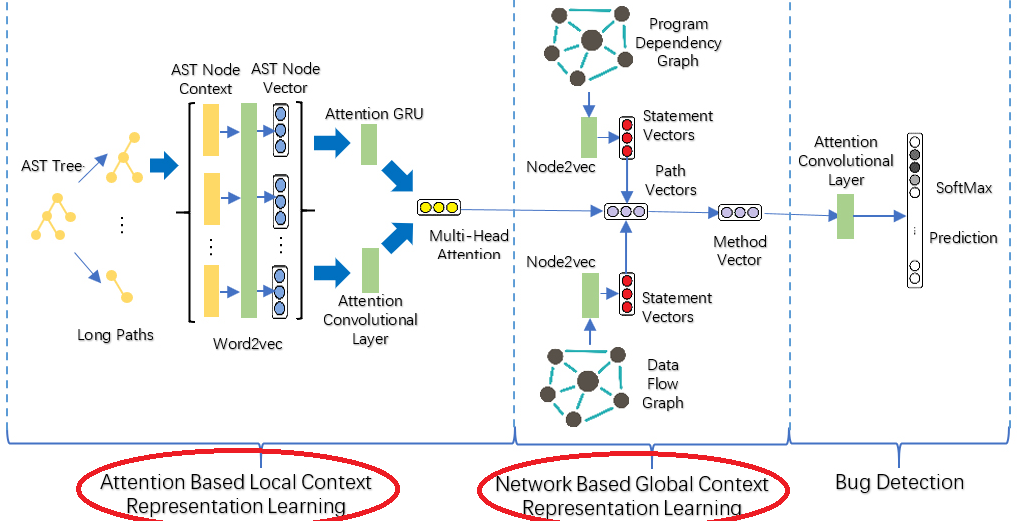
\includegraphics[height = 1.98in]{graphs/Graph_2_trim.png}
	\vspace{-22pt}
	\caption{Using Representation Learning for Bug Detection}
	\label{Fig.2}
%	\vspace{-10pt}
\end{wrapfigure}
(2) \textbf{Network-Based Global Context Representation Learning}.  We
also encode the method's context by building the PDG and the DFG
relevant to the method.
%We call them the \textbf{global context} as they provide the relations
%between the given method and other relevant methods in the project.
We use the Node2Vec~\cite{Grover-2016} to encode the PDG and DFG into
embedded vectors. These two vectors are combined by the space vectors
of all nodes in each path. We use matrix multiplication and convert
results together to get the path representation vector. Then, we can
have a method representation by appending all paths' vectors for each
method.  (3) \textbf{Bug Detection}. With both contexts for a method,
a classifier decides if the method is buggy or not. 

We plan to (1) investigate new CRL via our
framework to integrate program slices/reduction, symbolic traces, code
abstraction and intermediate representations; (2) explore new
embeddings and learning models for different level detection; (3) study new DL models on vectors from CRL to identify bugs.

%Our preliminary results~\cite{oopsla19} showed that with
%representation learning mechanisms (Figure~\ref{Fig.2}), our model
%significantly outperforms the one with the off-the-shelf
%Word2Vec-based CRL.

%\begin{wrapfigure}{r}{0.57\textwidth}
%	\vspace{-10pt}
%	\centering
%	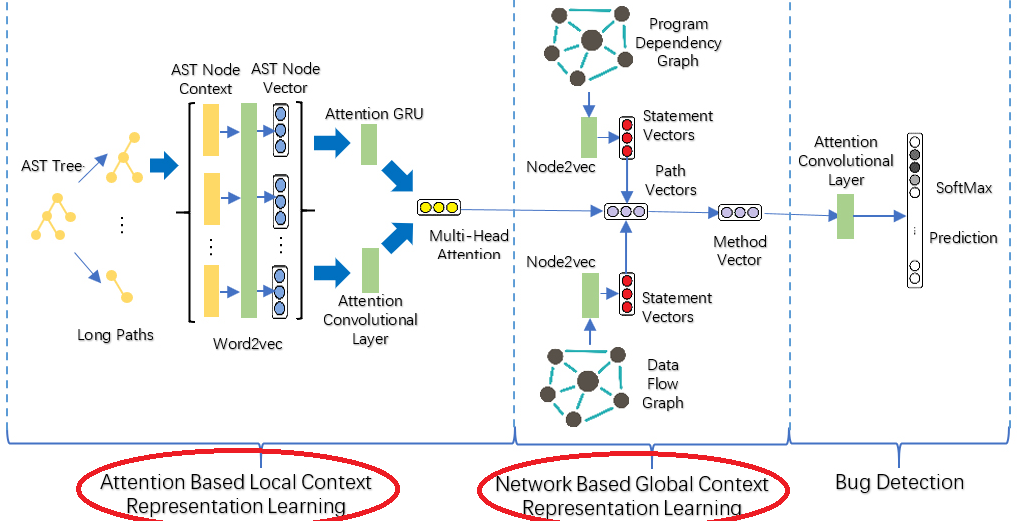
\includegraphics[scale=0.265]{graphs/Graph_2_trim.png}
%	\vspace{-25pt}
%	\caption{Using Representation Learning for Bug Detection}
%	\label{Fig.2}
%	\vspace{-15pt}
%\end{wrapfigure}

%Tien removed
%Table~\ref{allresults} show that (1) \textbf{our initial design
%  outperforms state-of-the-art baselines in detecting bugs},
%relatively improving DeepBugs, Bugram, NAR-miner, and FindBugs by
%69\%, 25\%, 92\%, and 156\% respectively in terms of F-score. (2)
%\textbf{our CRL with local and global contexts is more suitable than
%  existing CRL in bug detection}. It can improve relatively over all
%CLR baselines: DeepSim, DL-similarity, code2vec, Tree-based LSTM, Code
%Vectors,and GGM by 67\%, 38\%, 82\%, 206\%, 101\%, and 16.3\%,
%respectively, in terms of F-score. Importantly, our false positives
%rate is lower than others.
%\begin{wraptable}{r}{0.7\textwidth}
%	\vspace{-15pt}
%	{\footnotesize	
%		\caption{Ours Compared with BD Baselines and Existing CRL on BD. FP: False Positives}
%		\vspace{-10pt}
%		\begin{center}\label{allresults}
%			\renewcommand{\arraystretch}{1}
%			\begin{tabular}{p{1.2cm}<{\centering}|p{0.8cm}<{\centering}|p{0.8cm}<{\centering}|p{0.8cm}<{\centering}|p{1cm}<{\centering}|p{0.8cm}<{\centering}
%					|p{0.8cm}<{\centering}|p{0.8cm}<{\centering}|p{0.8cm}<{\centering}|p{0.8cm}<{\centering}|p{0.8cm}<{\centering}|p{0.8cm}<{\centering}} \cline{2-12}
%				
%				
%				\hline
%				\multirow{2}{*}{Category}& \multicolumn{5}{c|}{Bug detection baselines} & \multicolumn{6}{c}{Existing CRL on bug detection}\\
%				\cline{2-12}
%				& \textbf{Ours} & \textbf{DB} & \textbf{Bram} & \textbf{NARM} & \textbf{FB}   &\textbf{DS} & \textbf{DLS} & \textbf{C2V} & \textbf{TL} & \textbf{CV}&\textbf{GGM}\\
%				\hline
%				Recall  & 0.68 & 0.62 & 0.64 & 0.72 & 0.76   & 0.67 & 0.71 & 0.69 & \textbf{0.82} & 0.70&0.73\\
%				Precision& \textbf{0.39} & 0.25 & 0.32 & 0.11 & 0.08  &  0.19 & 0.24 & 0.17 & 0.09 & 0.15&0.30\\
%				F-score & \textbf{0.50} & 0.36 & 0.43 & 0.19 & 0.14 & 0.30 & 0.36 & 0.27 & 0.16 & 0.25&0.43\\
%				FP Rate & \textbf{0.21} & 0.41 & 0.39 & 0.52 & 0.66 & 0.35 & 0.36 & 0.43 & 0.69 & 0.45&0.28\\
%				\hline
%			\end{tabular}
%			DB=\deepbugs~2018: A deep learning bug detector; Bram=\bugram~2016: A n-gram model based detector;
%			NARM=\narminer~2018: A rule-based static detector mines negative rules on the code;
%			FB=\findbugs~2007: A rule-based static detector encoding +300 bug patterns.
%			DS, DLS, C2V, TL, CV, and GGM are defined in \textbf{Table 2}.
%			
%		\end{center}
%		\vspace{-25pt}
%	}
%\end{wraptable}

%Our initial results confirm that effective code representation learning (CRL) can help improve bug detection.



%Besides the basic CRs, e.g., identifiers/tokens/data and control
%flows/program dependency graph, we plan to investigate code
%representations obtained from more program analysis techniques (static
%and dynamic), such as program slices/reduction, symbolic traces, code
%abstraction, code intermediate representations (IR). Then, we combine
%the basic ones with the representations obtained from more static and
%dynamic program analysis techniques.  (2) Exploring new embeddings and
%learning models to propose new CRL approaches specialized for bug
%detection at different levels (i.e., variables, statements, and
%methods).  (3) Studying and proposing new deep neural networks on code
%vectors generated from CRL to identify bugs.


\subsection{T3 Task 2. Test Code Representation Learning for Regression Testing in CI}

%We use code representation learning to improve the
%selection and prioritization of test cases in Continuous
%Integration (CI)~\cite{duvall2007continuous}.
%
Regression Testing (RT) in Continuous
Integration~\cite{duvall2007continuous} (RT-CI) differs from the
traditional RT because most traditional RT techniques cannot be
applied at the scale of modern CI
practices~\cite{elbaum2014techniques} that require frequent commits to
the shared code base and cause the cost of continuous RT escalate
dramatically~\cite{memon2017taming}.
%
%RT-CI requires to identify and prioritize a subset of test cases that
%can timely and effectively uncover potential regression faults in the
%latest committed changes.
%
%Test selection and prioritization approaches in RT-CI are
%mainly in two directions: heuristics-based approaches
%(e.g.,~\cite{elbaum2014techniques,gligoric2015practical,yu2018study})
%and machine learning based approaches. However, existing approaches,
%e.g.,~\cite{bertolino2020learning,spieker2017reinforcement} still have
%limitations in accuracy and scalability as they lack the learning of
%deep features of test cases and source code and their relations.


%^Both only selection without prioritization or vise versa may be
%unsatisfactory, as time intervals among commits are very short and not
%all selected tests can be run or avoiding running many non-failing or
%irrelevant tests is the goal.
We will design a deep learning approach that leverages code representation
learning to select test cases and then prioritizes them in
each CI cycle.  
(1) \textbf{Test Selection.}  We use a hybrid strategy to select a subset of test cases, considering
static class-level dependencies among test cases and the ones between
changed source code and test cases, newly added test cases, diverse
test cases (e.g., \cite{jiang2009adaptive,henard2016comparing}). 
Static techniques are preferred over dynamic ones that are impractical
in CI due to runtime overhead~\cite{bertolino2020learning}. 
(2) \textbf{Test Prioritization.} Unlike previous approaches
(e.g.,\cite{bertolino2020learning}) modeling source code and test
history using hand-crafted metrics, we use CRL techniques (e.g.,
preferably unsupervised word embedding algorithms such as
Word2Vec~\cite{word2vec}, ELMo~\cite{peters2019knowledge},
FastText~\cite{bojanowski2017enriching}) to learn deep features of the
code under test to vectors, selected test cases, annotations for tests in code, 
similarities between
test cases and changed code, history-based test information (e.g., the
failed tests in the current commit and their similarities with the
changed code, the failed tests per test class in previous commits
before the current one, execution times).  Then, we utilize
learning-to-rank framework or active learning to prioritize test cases. 
In terms of
time complexity, existing approaches still have to generate graphs
(e.g., call/control graphs) for building metrics in a cycle, which can
take a longer time. In our approach, we build a language model
off-line and apply it on the natural sequences (or just tokens or AST)
of code under test into a vector in a cycle, which may not add overhead and even faster.  
Based on our previous experience, CRL can generate deeper and more representative
features than the hand-crafted metrics, leading to better results. 
We will further (1) investigate different
strategies for selection with CRL; (2) explore new fast and efficient
embeddings and learning models to propose new CRL approaches
specialized for RT-CI; (3) study to propose new practical
CRL-based approaches for test prioritization.



%study to propose a new off-line training for costly but potentially useful features and on-line prediction approach. 


%We exclude coverage-test selection and prioritization as they are very costly in CI due to the costs of instrumentation, recording and maintaining coverage data per release, in addition, they provide low accuracy due to the quick cycles and code changes


%different relationships: test cases dependency, dependency between test cases and source code, source code analysis for selecting and prioritizing test cases


\subsection{T3 Task 3. Code Coverage RL, Relation RL, and CRL for Fault Localization}

\begin{wrapfigure}{r}{0.45\textwidth}
	\vspace{-12pt}
	\centering
	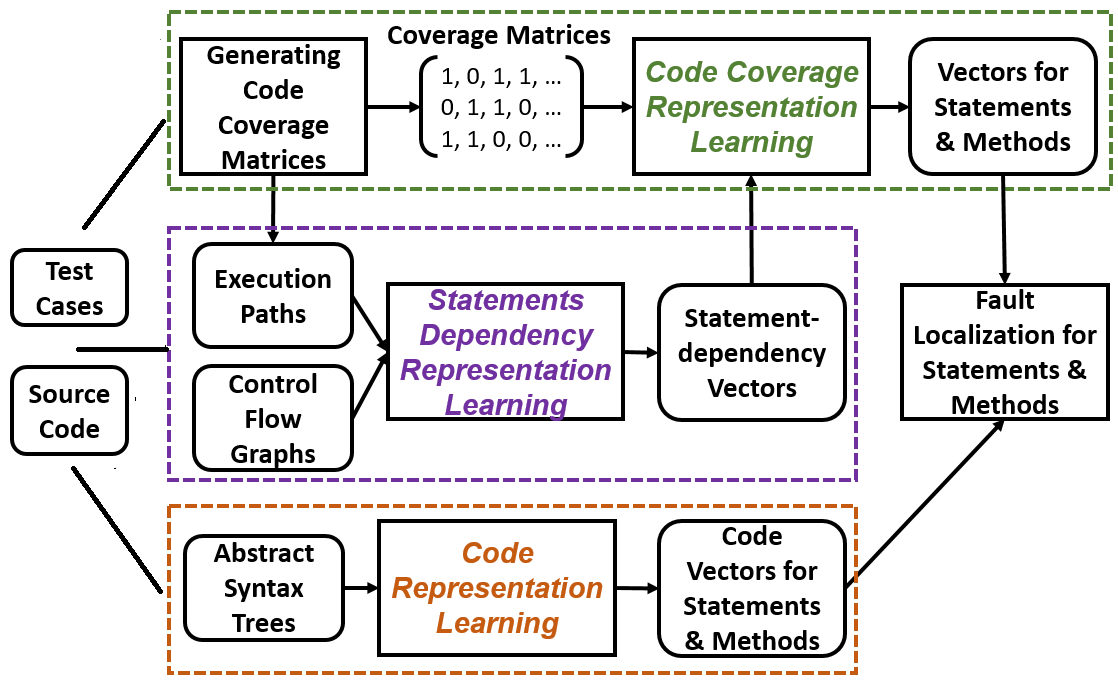
\includegraphics[height=1.8in]{graphs/newOverview}
	\vspace{-20pt}
	\caption{Using Representation Learning in FL.}
	\label{floverview}
	\vspace{-10pt}
\end{wrapfigure}
To experiment with CRL for dynamic information from program
executions, we propose a customized CRL for a fault localization
approach~\cite{icse_fl_21} at the statement and method levels.
%
%We use effective code and test coverage representation learning and
%novel deep neural networks for localizing faults at statement and
%method levels.
Our preliminary design~\cite{icse_fl_21} (Figure~\ref{floverview}) was
to leverage representation learning (RL) in three aspects. (1) {\bf
  code coverage representation learning}: Existing approaches
(spectrum-based, mutation-based, and deep learning-based approaches)
have never used the full details of test coverage, instead, they use
the spectrum and(or) mutation based formulas to summarize test
coverage for all test cases on each statement. We propose to {\em
  treat the FL problem as image processing by learning code coverage
  representations on the full details of the test coverage matrix}.
%Existing approaches (spectrum-based, mutation-based, and deep
%learning-based approaches) have never used the full details of test
%coverage, instead, they use the spectrum and(or) mutation based
%formulas to summarize test coverage for all test cases on each
%statement.
%To enrich test coverage matrices, we extract failing information of a
%test case and link it with specific code statements.  We use -1 for a
%failing test case at a statement exhibiting a crash or incorrect
%value.
%
%Next, while the rows representing statements are arranged according to
%the appearance order in the code, we order the columns, representing
%the test cases, so that the test coverages (i.e., the -1s, 0s, and 1s
%in the test coverage matrix) around the buggy statement would form a
%characteristic ``visual'' feature for a DL model to learn and detect
%it.  We directly perform RL on the improved matrices to learn vectors
%for statements or methods.  \underline{Second}, we integrate the
%dependencies/relations among the statements in the fault localization
%process using data dependency and execution traces.
(2) {\bf Statement dependency representation learning}: we aim to
learn the data/control dependencies among the statements. (3) {\bf
  code representation learning}: we also conduct CRL on sub-trees and
long paths of ASTs to generate vectors for source code. Finally, we
combine all three types of representation learning to represent a
statement or method by a vector representation. We will explore
different DL models for the classification purpose.~Preliminary
work shows that CNN works well for this classification of
a method/statement into buggy or not.

%(1) We prioritize test cases and mine failing information of test
%cases to enrich test coverage matrices and learn the code coverage
%representations; (2) We conduct the CRL on sub-trees and long paths of
%ASTs to generate vectors for source code, and also generate data flow
%graphs and run test cases to collect execution paths of code
%statements to learn the statement dependencies; (3) We combine the
%data flow graph and execution paths with improved matrices (spectrum
%and mutation), then apply a \cnn~on new matrices to learn vectors for
%an improved matrix.  We use another CNN on code vectors, vectors for
%the improved spectrum--based matrices, and vectors for the improved
%mutation-based matrices to perform fault localization (FL) at
%method-level. Our design can also work on statement-level FL by
%replacing the CRL at statement-level.


%\begin{table}[h]
%	\vspace{-15pt}
%	
%	{\footnotesize	
%		\caption{Our Approach Compared with FL Baselines at method-level and statement-level on Defects4J having 395 Bugs in total}
%		\begin{center}
%			\renewcommand{\arraystretch}{1}
%			\begin{tabular}{p{1cm}<{\centering}|p{0.8cm}<{\centering}|p{1cm}<{\centering}p{1cm}<{\centering}p{1cm}<{\centering}p{1.5cm}<{\centering}
%					p{1.2cm}<{\centering}p{1.5cm}<{\centering}|p{1.6cm}<{\centering}p{1.5cm}<{\centering}p{0.8cm}<{\centering}p{1.2cm}<{\centering}|p{0.8cm}<{\centering}} \cline{2-13}				\hline
%				\multirow{2}{*}{}& \multicolumn{7}{c|}{Fault Localization at Statement-Level} & \multicolumn{5}{c}{Fault Localization Method-Level}\\
%				\cline{2-13}
%				& \textbf{Ours} & \textbf{Ochiai} & \textbf{Dstar} & \textbf{MUSE} & \textbf{Metallaxis} &\textbf{RBF-NN} & \textbf{DeepFL-S} &\textbf{MULTRIC} & \textbf{FLUCCS} & \textbf{TraPT} & \textbf{DeepFL}&\textbf{Ours}\\
%				\hline
%				Top-1  & \textbf{74} & 17 & 19 & 26 & 24   & 16 & 36 & 80 & 160  & 156 & 213 &    \textbf{242} \\
%				MFR & \textbf{19.97}& 46.51 & 39.47 & 32.51 & 31.42 & 20.96 & 21.89  & 37.71 & 16.53 & 9.94 & 6.63 & \textbf{6.21}\\
%				\hline
%			\end{tabular}
%			RBF-NN: RBF Neural Network,
%			DeepFL-S: DeepFL with only features from spectrum+Mutation+MLP applicable to statements,
%			Top-1: the number of faults with a least one faulty element (statement or method) within top-1 position,
%			MFR: Mean First Rank of the localization of the first faulty element.
%			All method-level FL are machine learning (incl. deep learning) based.
%			\label{FL_S_M}
%		\end{center}
%		\vspace{-20pt}
%	}
%\end{table}


%Table~\ref{FL_S_M} show that our initial approach outperformed all baselines at both statement and method levels. Compared with the best performing statement-level and method-level baseline: DeepFL-S and DeepFL, we improved them by 115\% and 14\%, respectively. Our key ideas of designing representation learning for code and test coverage can help improve the current state-of-the-art FL research.

%To expand our initial design, we will (1) derive new code representations for FL; (2) Explore new embeddings and learning models to propose new code representation learning (CRL) approaches for FL; (3) Study and proposing new deep neural networks to localize faults.

\subsection{T3 Task 4. Code Transformation Learning for Automated Program Repair}

In this task, we aim to improve DL-based APR approaches via effective
CRLs, particularly {\bf Code Transformation Learning}.
%to improve the current deep-learning (DL) and pattern APR approaches
%using effective CRL and novel deep neural networks.  The DL-based
%approaches, e.g.,~\cite{hata2018learning,lutellier2020coconut}, still
%have limitations in learning bug-fixing code changes and learning
%which context of the surrounding source code that certain bug-fixing
%changes should be made.  These limitations lead to incorrect fixing
%locations or incorrect fixes.
We initially designed a two-tier DL model, \tool~\cite{icse_fl_20}, to
treat APR as code transformation learning from the prior bug fixes and
the surrounding code contexts of the fixes.
%
%For training, {\tool} has 5 key steps: {\bf (1) Pre-Processing.}
%First, {\tool} performs alpha-renaming on the names of variables
%within a method of a project.  Second, , {\tool} uses
%Word2Vec~\cite{Mikolov-2013} to train a vector representation for each
%unique token in a given pair of buggy method ($M_b$) and its fixed
%version ($M_f$).  {\tool} identifies the buggy sub-tree ($T^{sub}_b$)
%within $M_b$, and $T^{sub}_b$'s corresponding changed sub-tree
%($T^{sub}_f$) within $M_f$.  Finally, we used a code summarization
%model~\cite{wan-ase18} to summarize a tree into a vector for a node
%({\em a summarized node}). We obtain one vector for $T^{sub}_f$ and
%another one for $T^{sub}_b$.
{\bf (1) Code Context Learning.} We designed a two-layer learning model
that leans the code transformations for bug fixes and the context of
the code surrounding the fixes. The first one is dedicated for local
\textbf{C}ontext \textbf{L}earning \textbf{L}ayer (CLL).
%
For training at this layer, we replace the changed sub-tree with
a {\em summarized node}, as well as the buggy
sub-tree.  Given pre-processed pairs of methods, we developed a
tree-based encoder-decoder model using tree-based
LSTMs~\cite{tai2015improved} for this local context learning.  We
compute the vector for a method AST with the summarized node in a pair
of methods ($M_b$, $M_f$). The obtained vectors are used as the weights
in the next step. {\bf (2) Code Transformation
	Learning.}  The second layer is dedicated to code
\textbf{T}ransformation \textbf{L}earning \textbf{L}ayer (TLL) for
bug-fixing changes. In TTL, the changed sub-tree before and after the
fix is used for training to learn the bug-fixing code
transformations. Moreover, the context of the transformation computed
as the vector in the context learning layer is used as an additional
input in this~step.
%Specifically, we use the same tree-based encoder-decoder model in the
%first layer, CLL, to encode both structural and token changes.  {\bf
%  (4) Program Analysis Filtering.}  {\tool} derives the possible
%candidates using program analysis filters, including the filter to
%check the existence of variables, methods, and class names, the filter
%to convert the keywords back to the right names, and the filter to
%check the syntax of final result.  {\bf (5) Patch Re-ranking.} We use
%a CNN~\cite{kim2014convolutional} based classification approach to
%re-rank the generated possible patches based on the detailed
%contextual information, which helps better selecting the results.

We also have the following tasks in this thrust: (1) Investigating new
code representations for APR using our code representation learning
(CRL) framework; (2) Exploring new embeddings and learning
models to propose new CRL approaches specialized for APR; and (3)
Studying and even proposing new deep neural network models to auto-fix
multi-statements and multi-location bugs.

%In our initial design, our DLFix is novel in two ways: new CRL and a
%new two-layer tree-based encoder-decoder model.




%\input{benchmark}

%\input{model}
%\input{mudetect}

%\input{solution}


\section{Evaluation Plan}
\label{eval}

%Our {\em goals} of the evaluation plan include the studies to answer the questions:

%1) {\bf Intrinsic evaluation.} 

%2) {\bf Extrinsic evaluation.} How well do our proposed tools and methods help developers in improving the learning and usages of APIs in software libraries?

%3) How effectively do the proposed tools and methods help developers
%in real development processes?

This following evaluation plan will help ensure that our framework meets
the needs of VIPLs.

%and provides them with a powerful and accessible programming environment.

{\em 1. User Recruitment and Selection:} Recruit a diverse group of
visually-impaired programmers and learners who have varying levels of
programming experience, from beginners to experts.  Ensure that the
participants represent a range of age groups and backgrounds to
capture different user perspectives. We ensure that all participants
provide informed consent and understand the nature of the study.
Respect privacy and confidentiality concerns, especially when dealing
with sensitive voice data.

{\em 3. Experiment Tasks:} Create a series of experiments to evaluate
different aspects of the Voice-Driven Programming Framework.  Ensure
that the experiments cover both the voice interaction and code
generation components of the environment. We will conduct user testing
sessions where participants interact with the Voice-Driven Programming
Framework to complete various programming tasks.  Record and analyze
user interactions, including voice commands and modifications to
generated code.  Gather user feedback through interviews and surveys
after each testing session. {\em Error Handling and Debugging:}
Evaluate the effectiveness of voice commands for debugging, error
detection, and resolution.

{\em 4. Evaluation Metrics:} Define clear and measurable metrics to
assess the performance and usability of the framework. Possible
metrics include: Code accuracy: Measure the correctness of code
generated by the framework.  Task completion time: Assess how quickly
users can perform common programming tasks.  Error detection: Evaluate
the framework's ability to help users identify and correct errors.
User satisfaction: Gather user feedback through surveys and interviews
to gauge overall satisfaction and user experience.  Accessibility:
Assess how well the environment accommodates the needs of
visually-impaired users.

{\em 5. Accessibility Testing:} Conduct accessibility tests to ensure
that the framework complies with accessibility standards, such as WCAG
(Web Content Accessibility Guidelines).Involve visually-impaired
accessibility experts in the testing process. {\em Collaboration and
  Documentation Assessment:} Evaluate the framework's ability to
support collaborative coding by involving participants in
collaborative coding exercises.  Assess the effectiveness of
voice-driven documentation creation.

{\em 6. User Learning Curve:} Assess how quickly users adapt to and
become proficient in using the Voice-Driven Programming
Framework. Long-term Usability: Conduct follow-up evaluations with
participants over an extended period to assess the framework's
usability and effectiveness in real-world scenarios.

{\em 7. Comparative Analysis:} Compare the performance of our
framework against traditional screen readers and code editors for
visually-impaired users. Analyze the collected data to draw meaningful
conclusions regarding the framework's strengths, weaknesses, and areas
for improvement.
%Compile a detailed report
%summarizing the findings, including quantitative data, user feedback,
%and suggestions for enhancements.
From the evaluation results, continue to refine and enhance the
environment, addressing identified issues and incorporating user
suggestions.  Ensure that the environment adheres to accessibility
standards and guidelines for VIPLs.

{\em 8. Iterative Improvement:} Use the feedback and data collected
from each testing session to make iterative improvements to the
environment.  Continuously refine all the components
%the voice recognition, code
%generation, and user interface components
based on user input.

{\em 9. Public Testing and Feedback:} Consider conducting a public
beta test to gather feedback from a wider audience of
visually-impaired users, potentially expanding the diversity of
participants.





\section{Dissemination and Educational Plan}
\label{edu}

\paragraph{Engaging Students into Research}

This project will create opportunities for students at UT-Dallas to
participate into cutting-edge research: PI Nguyen has currently supported
four female students (2 PhD students and 2 undergraduates), with a total
of four PhD students, two M.Sc. students, and four undergraduates.

%has worked with 6 undergraduate students (i.e., two are female
%students) and two master students (i.e., independent
%study). Additionally, PI Wang is actively doing research with a group
%of two undergraduate students (Vrushali Koli (female) from NJIT and
%Delmond Wyllis from Rowan Univ. in NJ) and \underline{six high-school
%students} in the NJ Governor's STEM Scholars Program.  PI Wang
%supervise 4 Ph.D students (one female) and 1 master student.


%(2) {\em UTD's Collegium Honors Program}:
%{\em ISU's Freshman Honor program}: 
%PI Nguyen has been engaging two freshman honor students into his
%research program since he joined UTD in 2016. 
%REU supplements will be requested to support this undergraduate research; 
%
%(3) {\em HackersUTD}: This Fall, UT Dallas Computer Science department
%welcomed 2,876 students, including 466 CS/software engineering
%freshmen, with activities and events as a way to welcome and
%familiarize students with the UT Dallas CS. We will engage members of
%this organization; 
%(3) UT Dallas works with North Texas high school
%seniors to host IT empowerment for their camps. To generate interests
%in computing studies from {\em high-school} students in Dallas area,
%we will involve them in design projects that target the use of
%software in teaching {\em K-12} subjects; 
%(2) {\em UTD's Women Who
%Compute}: The PI Nguyen has actively used this program to generate interests
%in SE research from women students. From the past, PI Nguyen has
%mentored 3 women students; 
%(Dong Fei, Kristina Gervais, Taylor Schreck); 
%(3) {\em Involving Under-represented Minorities}: We
%will attract minority students funded by GEM fellowships, involve
%high-school teachers via Alliances for Graduate Education and the
%Professoriate.
%and UT Dallas Programs for Minors: we will work
%with this program to recruit more student in minority.

%This project will also create opportunities for students at UT-Dallas:
PI Nguyen has extensive experience in engaging students in outreach
programs: (1) {\em Collaborative educational project between UT-Dallas
and Fulbright University Vietnam (FUV)}: Through this program, PI
Nguyen has been mentoring a honor thesis project for two undergraduate
students that has been conducting the preliminary empirical study
described in Section~\ref{sec:thrust1}. PI Nguyen is also a mentor for
two visually-impaired students at FUV, Tran Viet Hoang and Tran Trong
Nghia, who have been extremely helpful for our preliminary study.
(2) {\em UTD's Collegium Honors Program}: He
has been engaging several freshman honor students into his research
program since 2005. (3) {\em HackersUTD}: In Fall'19, UT Dallas CS
welcomed 2,876 students, including 466 freshmen, with activities and
events as a way to familiarize students with CS/SE. We will use the
results of this project in this program.
%
(4) UT Dallas works with {\em North Texas high school seniors to host
IT empowerment} for their camps. To generate interests in computing
studies from {\em high-school} students in Dallas area, PI Nguyen has
been involving them in design projects that target the use of software
in teaching {\em K-12} subjects; (5) {\em UTD's Women Who Compute}: he
has actively used this program to generate interests in SE research
from women students. PI Nguyen has mentored several {\em female
undergraduate students} (Weining Gao, Kristina Gervais, Taylor
Schreck, etc.); Currently, he supervise two undergraduate students
(Dao Ngoc, Nam Anh) and two female PhD students (Mary Grace Kozuch and
Hridya Dhulipala) (6) {\em Involving Under-represented Minorities}: We
will attract minority students funded by GEM fellowships, involve
high-school teachers via Alliances for Graduate Education and the
Professoriate; and (7) {\em UT Dallas Programs for Minors}: we will
work with this program to recruit more student in minority.


\paragraph{Dissemination of Research and Teaching Materials}

Beside publications at professional \emph{conferences, journals} and
public Web sites, we will explore:
%$use the available resources at UT-Dallas
%through various forums for dissemination.
%
%PI Wang is a member of DIMACS~\cite{dimacs}, the Center for Discrete
%Mathematics and Theoretical Computer Science as an NSF-funded Science
%and Technology Center (STC) and a New Jersey Commission on Science and
%Technology Advanced Technology Center. DIMACS has over 350 members
%across the U.S. PI Wang will continue to advocate our research through
%DIMACS events, research and academic programs.  PI Wang will use
%the \textit{annual NJIT Research Showcase and President Forum} to show
%our accomplishments to all NJIT people.
%PI Nguyen will continue to use the following resources:
(1) TExAs Software Engineering Research (TEASER) Doctoral Symposium:
where SE researchers from the DFW Metroplex (and beyond) meet to
discuss and work on SE topics.  The mission of TEASER is to provide a
supportive space in which PhD students can present and receive
feedback on their research work, while at the same time giving both
researchers and students a venue to get to know one another and
network productively.  (2) American Society for Engineering Education:
PI Nguyen, with his prior NSF-funded TUES project, has disseminated
educational results via this channel.
%He will continue to disseminate educational outcomes via this
%educational society.
(3) Leadership through Engineering Academic Diversity (LEAD): PI
Nguyen have served as mentors for this program which aims to enrich
educational experience of {\em minority engineering students}.

%\paragraph{Research Community Building.}

%PI Nguyen has successfully organized the 1st {\bf International
%Workshop on Representation Learning for Software Engineering and
%Programming Languages (RL+SE\&PL 2020)}~\cite{rlsepl}, associated with
%ESEC/FSE'20. The workshop had 104 paid registers and featured one
%keynote speaker (Dr. Miltos Allamanis, well-known CRL scientist at
%Microsoft Research) and six technical presentations. RL+SE\&PL'20 has
%sparked constructive and inspiring discussions. With its success, we
%are building a diverse and active community. We plan to build on the
%success of the first edition to continue this series to disseminate
%ideas to a wider community, and to build a larger community bridging
%SE and ML.

%\section{Education and Dissemination Plan - Curriculum Development Activities}


\noindent {\bf Undergraduate and Graduate Software Engineering (SE) Education.} 
%PI Wang teaches fundamental and core SE courses NJIT: Building Web Applications (IS218) and System Design (IS390).
PI Nguyen is one of the key SE faculty members in the BS, MS, and Ph.D.
degree programs in SE at UT Dallas. 
%
He is one of the faculty who has initiated and contributed to
Undergraduate SE Program when he was at Iowa State University.
%He has
%successfully introduced several courses including Software
%Architecture and Design (CprE339) and Software Project Management
%(CprE329). 
Taking advantage of this project, PI Nguyen will introduce a deep
learning component and a new course in NLP+SE.
The key teaching philosophy in this course is the combination of theory and practice.
%in which students will be introduced different principles and theories in the application of NLP in SE artifacts. 
%The tentative modules include 1) basic principles, processes, and paradigms in NLP, 2) programming languages versus natural languages, 3) API usages and reuse, 4) Statisical models used in SE applications, 5) machine translation and code migration, 6) language models for source code, 7) applications of machine translation in SE, 8) word embeddings and SE applications, 9) deep learning and SE applications, etc.
%\noindent {\em Graduate SE Education} 
PI Nguyen will teach a newly developed course, 
Selected Topics on AI in SE and PL,
including relevant topics to this proposal, e.g, 
AI in bug detection, fault localization, automated repair. 
%The PI Nguyen works
%with other UTD faculty to develop a series of six to seven SE graduate
%courses that will be offered at least every semester. This year, the
PI Nguyen introduced a new graduate level course on ``AI/ML for
Code''. The PI will introduce a new graduate course on the topic of
NLP+SE.
%Tools developed by this research will be used in class projects. 
The course will focus on several SE advanced methods that
aim to help advance software engineering with AI/ML techniques. 
The tentative topics include 1) program analysis, 2) source code
analysis with AI/ML, 3) cross-language analysis between texts and code,
4) AI/ML for code, etc.
%4) code and text retrieval in SE applications, 
%3) NLP techniques and
%type inference, 4) NLP and de-ofuscation, 5) bug-fixing and
%machine learning.




\section{PI's Prior Relevant NSF Supports and Qualifications for this Project}
\label{prior}

%PI Wang has no prior relevant NSF supports.
%His relevant work on improving software maintenance, quality and reliability has been published in
%OOPSLA~\cite{yioopsla19}, ASE~\cite{son-2019-ase}, EMSE~\cite{noei2019towards,wang2016improving}, ICWS~\cite{venkatesh2016client}, ICSOC~\cite{wang2014developers}, and MSR~\cite{wang2013improving,wang2019extracting}.
%two ICSE submissions, and one PLDI submission.

PI Nguyen. CNS-2120386, \$448,168, 10/01/2021 - 09/30/2024,
``Collaborative Research: CCRI: ENS: Boa 2.0: Enhancing Infrastructure
for Studying Software and its Evolution at a Large Scale''.
\noindent {\bf Intellectual Merit.} Building an infrastructure for
software mining including AI/ML capabilities.
\noindent {\bf Broader Impact.}  The project has several publications
at top-tier SE conferences, e.g., ICSE, FSE, ASE, TSE.  He has been
awarded {\bf 4 ACM SIGSOFT Distinguished Paper Awards, one Best Paper
  Award, and one best ICSE Formal Research Demonstration Award} at the
top-tier SE conferences including ICSE, FSE, and ASE, one {\bf IEEE
  TCSE Distinguished Paper Award}. He has served on Program Committees
and Program Boards of ICSE, FSE, ASE, OOPSLA, ECOOP. PI Nguyen was a
Program Co-Chair of ASE'17.

%Since 2005, PI Nguyen published at the top-tier Software Engineering
%conferences including 21 ICSE full papers, 12 ESEC/FSE full papers, 13
%ASE full papers, 3 OOPSLA full papers.
%From Google Scholar, PI
%Nguyen's H-index is 49, Citations: 9,431, Citations in past 5-years:
%5,879. From CSRankings.org, he is ranked at the 3rd place among all
%Software Engineering researchers in the US in the past 10 years.



%making software development more accessible, enjoyable and productive;
%and therefore will broadly enhance the value that software
%professionals deliver to business and society.

%Dr. Nguyen is currently the PI of the NSF-funded project, ``
%Collaborative Research: Exploiting the Naturalness of Software'', that
%will end August 2018. The work has three thrusts of research.  (1)
%Investigating the integration of semantic information including data
%types, semantic roles, etc., into a language model, (2) Developing an
%accurate code-completion tool using statistical semantic language
%model, and (3) Developing a statistical machine translation model for
%language migration. So far, the majority of the tasks have been
%%completed except empirical evaluation in a real-word setting is
%needed.



%Several papers on our results were published through ICSE
%2010~\cite{icse10}, ASE 2010~\cite{ase10}, OOPSLA
%2010~\cite{oopsla10}, ICSM 2010~\cite{icsm10}, ICSE
%2011~\cite{icse11,nier11-1,nier11-2}, FSE 2011~\cite{fse11}, ASE
%2011~\cite{ase11-phpsync,ase11-bugscout,ase11-idiff}, and an IEEE TSE
%journal article~\cite{tse11}.

%Our next phase will be involved more with the tasks (2) and (3).

%Dr. Nguyen is currently an PI on a NSF-funded project: \#CCF-1018600,
%``Find and Fix Similar Software Bugs'', 08/15/2010 through
%07/31/2013. In this project, an empirical study will be conducted to
%collect, analyze, and understand the nature and characteristics of
%recurring and similar bugs within one and across multiple
%systems. This project is expected to advance software engineering
%knowledge on the theoretical foundation, concepts, practical
%techniques, and automated tools to (1) capture the characteristics and
%measure the similarity of code units involved in prior known fixed
%bugs, (2) identify the locations of potential buggy units and derive
%the guidelines to fix them by matching them to the relevant peer code
%units of the known bugs, and (3) support the similar bug detection and
%fixing process. Teaching modules and validation efforts in this
%project will involve students and professionals, promoting teaching
%and training software quality assurance.

%Dr. Nguyen is an expert in software building, software configuration
%management (SCM), and software refactoring. His research work on SCM
%has been published at various prestigious software engineering
%journals and conferences including clone-aware configuration
%management and operation-based version control (TSE'11~\cite{tse11},
%FASE'10~\cite{fase10}, ASE'09~\cite{ase09}), software
%refactoring-aware SCM and software merging (TSE'08 \cite{tse08},
%ICSE'07~\cite{icse07}, FSE'06~\cite{fse06}, OOPSLA'06
%demo~\cite{oopsla06}), object-oriented configuration management
%(ICSE'07~\cite{icse07}, WWW'06~\cite{www06}, ICSE'05~\cite{icse05},
%ICSM'05~\cite{icsm05}).

%His other software maintenance works include clone-related bug
%detection (TSE'11 \cite{tse11}), bug localization
%(ASE'11~\cite{ase11-phpsync}), bug localization from bug reports
%(ASE'11~\cite{ase11-bugscout}), recurring bug detection
%(ICSE'10~\cite{icse10}), API misuse detection
%(OOPSLA'10~\cite{oopsla10}, FSE'09~\cite{fse09}), recurring
%vulnerabilities detection (ASE'10~\cite{ase10}), etc.




%Since 2005, his work has been resulting several publications at
%top-tier SE conferences including 5 ICSE
%papers~\cite{icse05,icse07,icse09,icse10,icse11}, 3 FSE
%papers~\cite{fse06,fse09,fse11}, 8 ASE
%papers~\cite{ase06,ase08,ase08-2,ase09,ase10,ase11-phpsync,ase11-bugscout,ase11-idiff},
%2 WWW papers~\cite{www04,www06}, 3 OOPSLA
%papers~\cite{oopsla04,oopsla06,oopsla10}, and 2 FASE
%papers~\cite{fase09,fase10}, 2 TSE papers~\cite{tse08,tse11}.


\newpage
\setcounter{page}{1}
\pagenumbering{roman}

\bibliographystyle{IEEEtran}
%\nobibliography{oopsla19,icse20,FL,ref,autofixTools}
\bibliography{oopsla19,icse20,FL,ref,autofixTools,testPri,embeddingEva,reference,icse21IntVD,icse18}

%\bibliography{oopsla19, icseAutoFix20,bibliography,icse18,t2api17,ccf18,refs,securesync,tc10,tien,ccf09,ase10,ccf12,anomalies,completion,groums,usagemining,pattern,urls,other}

\end{document}
